\documentclass{notes}

\title{Notes on navigation history}
\author{Alan Jeffrey \and Connor G. Brewster}
\date{DRAFT of 2016-06-23}
\indicia{
  
\includegraphics[height=4.5ex]{images/by}
  \begin{tabular}[b]{@{}l}%
    Copyright Alan Jeffrey and Connor G. Brewster\\
    Licensed under Creative Commons License CC-BY
  \end{tabular}
}

\usepackage{amssymb}
\usepackage{graphicx}
\usepackage{float}
\usepackage{subcaption}
\usepackage{tikz}
\usetikzlibrary{fit}

% Macros, so we can change notation easily
\newcommand{\aNH}{H}
\newcommand{\Docs}{D}
\newcommand{\Active}{A}
\newcommand{\FullyActive}{F\!A}
\newcommand{\parentOf}{\rightarrow}
\newcommand{\parentOfActive}{\twoheadrightarrow}
\newcommand{\childOf}{\larrow}
\newcommand{\activeChildOf}{\twoheadleftarrow}
\newcommand{\leChron}{\le}
\newcommand{\ltChron}{<}
\newcommand{\geChron}{\ge}
\newcommand{\gtChron}{>}
\newcommand{\eqSess}{\sim}
\newcommand{\ltSess}{\lesssim}
\newcommand{\gtSess}{\gtrsim}
\newcommand{\rootDoc}{d_0}
\newcommand{\aDoc}{d}
\newcommand{\bDoc}{e}
\newcommand{\cDoc}{f}
\newcommand{\st}{\mathbin.}
\newtheorem{goal}{Goal}
\newtheorem{patch}{Patch}
\newtheorem{counterexample}{Counterexample}
\newtheorem{experiment}{Experiment}

\tikzstyle{doc} = [draw=black, fill=blue!10, circle, font={\normalfont\sffamily}]
\tikzstyle{fully} = [draw=red, thick]
\tikzstyle{active} = [color=white, fill=blue!50!black]
\tikzstyle{jshactive} = [active] % ASAJ: if we want jshactive to be distinct [fill=green!50]

\begin{document}

\maketitle

\subparagraph{Abstact:}
Some notes on a model of navigation history.

\subparagraph{ACM Classification:}
D.2.1 Requirements/Specifications.

\subparagraph{Keywords:}
Formal model,
Navigation,
Session history,
Specification,
Web browsers.

\section{Introduction}

[These are rough notes, working towards a model of navigation history for the web.]

\section{Preliminaries}

[Define forest, tree, root, total order, equivalence.]

\section{Model}

A \emph{navigation history} $\aNH=(\Docs,\Active,{\parentOf},{\leChron},{\eqSess})$ consists of:
\begin{itemize}
\item a set $\Docs$ (the \emph{documents}),
\item a subset $\Active \subseteq \Docs$ (the \emph{active} documents),
\item a forest $(\Docs,{\parentOf})$ (the \emph{document hierarchy}),
\item a total order $(\Docs,{\leChron})$ (the \emph{chronological order}), and
\item an equivalence relation $(\Docs,{\eqSess})$ (the \emph{same-session equivalence}).
\end{itemize}
such that:
\begin{itemize}
\item for every $\aDoc$ there is a unique $\aDoc'\in\Active$ such that $\aDoc \eqSess \aDoc'$,
\item for every $\aDoc \parentOf \bDoc \eqSess \bDoc'$
  we have $\aDoc \parentOf \bDoc'$, and
\item for every $\aDoc \parentOf \bDoc$, we have $\aDoc \leChron \bDoc$.
\end{itemize}
Define:
\begin{itemize}
\item $\rootDoc$ is the unique active root document,
\item $\aDoc \parentOfActive \bDoc$ when $\aDoc \parentOf \bDoc$ and $\bDoc \in \Active$,
\item $\FullyActive = \{ \aDoc \mid \rootDoc \parentOfActive^* \aDoc \}$
  (the \emph{fully active} documents),
\item $\aDoc \ltSess \bDoc$ whenever $\aDoc \eqSess \bDoc$ and $\aDoc \ltChron \bDoc$,
\item the \emph{session future} of $\aDoc$ is $\{ \bDoc \mid \aDoc \ltSess \bDoc \}$,
\item the \emph{session past} of $\aDoc$ is $\{ \bDoc \mid \aDoc \gtSess \bDoc \}$,
\item the \emph{joint session future} is $\{ \bDoc \mid \exists \aDoc \in \FullyActive \st \aDoc \ltSess \bDoc \}$,
\item the \emph{joint session past} is $\{ \bDoc \mid \exists \aDoc \in \FullyActive \st \aDoc \gtSess \bDoc \}$,
\end{itemize}
Define \emph{deleting $\aDoc$ from $\aNH$}, when $\aDoc\not\in\FullyActive$, to be $\aNH'$ where:
\begin{itemize}
\item $\Docs' = \aDoc \setminus \{ \bDoc \mid \aDoc\parentOf^* \bDoc \}$,
\item $\bDoc\in\Active'$ whenever $\bDoc\in\Active$,
\item $\bDoc\leChron'\cDoc$ whenever $\bDoc\leChron\cDoc$,
\item $\bDoc\parentOf'\cDoc$ whenever $\bDoc\parentOf\cDoc$, and
\item $\bDoc\eqSess'\cDoc$ whenever $\bDoc\eqSess\cDoc$.
\end{itemize}
Define \emph{replacing $\aDoc$ by $\aDoc'$ in $\aNH$}, where $\aDoc\in\Active$ and
$\aDoc'\notin\Docs$, to be $\aNH'$ where:
\begin{itemize}
\item $\Docs' = \Docs \cup \{\aDoc'\}$,
\item $\bDoc \in \Active'$ whenever
  $\bDoc \in \Active$ and $\bDoc\ne\aDoc$, or
  $\bDoc=\aDoc'$,
\item $\bDoc \leChron' \cDoc$ whenever
  $\bDoc \leChron \cDoc$, or $\cDoc = \aDoc'$,
\item $\bDoc \parentOf' \cDoc$ whenever
  $\bDoc \parentOf \cDoc$, or
  $\bDoc \parentOf \aDoc$ and $\cDoc = \aDoc'$, and
\item $\bDoc \eqSess' \cDoc$ whenever
  $\bDoc \eqSess \cDoc$, or
  $\bDoc \eqSess \aDoc$ and $\cDoc = \aDoc'$, or
  $\aDoc \eqSess \cDoc$ and $\bDoc = \aDoc'$.
\end{itemize}
Define \emph{navigating from $\aDoc$ to $\aDoc'$ in $\aNH$} to be the result of:
\begin{itemize}
\item deleting the session future of $\aDoc$, and
\item replacing $\aDoc$ by $\aDoc'$.
\end{itemize}
Define \emph{traversing the history to $\aDoc$ in $\aNH$} to be $\aNH'$ where:
\begin{itemize}
\item $\Docs'$ is $\Docs$,
\item $\bDoc\in\Active'$ whenever $\aDoc\not\eqSess\bDoc \in \Active$, or
  $\aDoc=\bDoc$,
\item $\bDoc\leChron'\cDoc$ whenever $\bDoc\leChron\cDoc$,
\item $\bDoc\parentOf'\cDoc$ whenever $\bDoc\parentOf\cDoc$, and
\item $\bDoc\eqSess'\cDoc$ whenever $\bDoc\eqSess\cDoc$.
\end{itemize}
Define \emph{$\aNH$ traverses the history by $+\delta$ to $\aNH'$} when:
\begin{itemize}
\item the joint session future of $\aNH$ is $\aDoc_1 \gtChron \cdots \gtChron \aDoc_\delta \gtChron \cdots$,
\item $H$ traverses the history to $d_\delta$ in $H'$
\end{itemize}
Define \emph{$\aNH$ traverses the history by $-\delta$ to $\aNH'$} when:
\begin{itemize}
\item the joint session past of $\aNH$ is $\aDoc_1 \ltChron \cdots \ltChron \aDoc_\delta \ltChron \cdots$,
\item $H$ traverses the history to $d_\delta$ in $H'$
\end{itemize}
Define \emph{$\aNH$ traverses the history by $0$ to $\aNH'$} when $\aNH=\aNH'$.

[This defn is meant to align with the spec.]

\section{Properties}


[State some goals, e.g. go($\delta$);go($\delta'$) is the same as go($\delta+\delta'$),
  navigate;go($-1$) has the same fully active documents as doing nothing,
  session history can be implemented effeciently in memory...]

[I suspect none of these are true of the current spec, can we find a model in which
  they are true?]

\begin{goal}
\label{goal:homomorphism}
  If $H$ traverses the history by $\delta$ to $H'$
  and $H'$ traverses the history by $\delta'$ to $H''$
  then $H$ traverses the history by $\delta+\delta'$ to $H''$.
\end{goal}

\begin{counterexample}
  \label{counterexample:homomorphism1}
  Let $H$ be:
  \[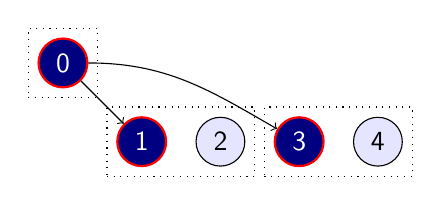
\begin{tikzpicture}
    \node[doc,active,fully](0) at (0,0){0};
    \node[doc,jshactive,fully](1) at (1,-1){1};
    \node[doc](2) at (2,-1){2};
    \node[doc,active,fully](3) at (3,-1){3};
    \node[doc](4) at (4,-1){4};
    \node[draw,dotted,fit=(0)] {};
    \node[draw,dotted,fit=(1)(2)] {};
    \node[draw,dotted,fit=(3)(4)] {};
    \draw[->](0)--(1);
    \draw[->](0)to[out=0,in=150](3);
  \end{tikzpicture}\]
  which traverses the history by $1$ to:
  \[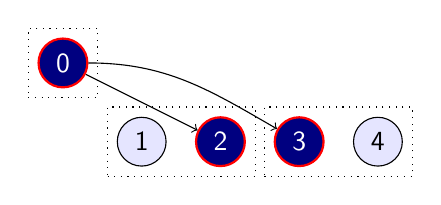
\begin{tikzpicture}
    \node[doc,active,fully](0) at (0,0){0};
    \node[doc](1) at (1,-1){1};
    \node[doc,jshactive,fully](2) at (2,-1){2};
    \node[doc,active,fully](3) at (3,-1){3};
    \node[doc](4) at (4,-1){4};
    \node[draw,dotted,fit=(0)] {};
    \node[draw,dotted,fit=(1)(2)] {};
    \node[draw,dotted,fit=(3)(4)] {};
    \draw[->](0)--(2);
    \draw[->](0)to[out=0,in=150](3);
  \end{tikzpicture}\]
  which traverses the history by $1$ to:
  \[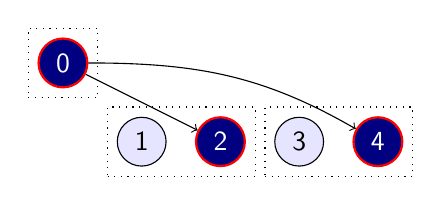
\begin{tikzpicture}
    \node[doc,active,fully](0) at (0,0){0};
    \node[doc](1) at (1,-1){1};
    \node[doc,active,fully](2) at (2,-1){2};
    \node[doc](3) at (3,-1){3};
    \node[doc,jshactive,fully](4) at (4,-1){4};
    \node[draw,dotted,fit=(0)] {};
    \node[draw,dotted,fit=(1)(2)] {};
    \node[draw,dotted,fit=(3)(4)] {};
    \draw[->](0)--(2);
    \draw[->](0)to[out=0,in=150](4);
  \end{tikzpicture}\]
  but $H$ traverses the history $2$ to:
  \[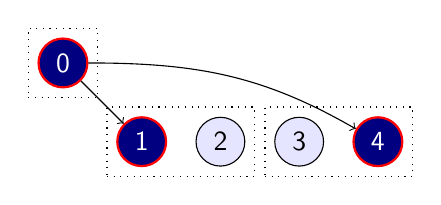
\begin{tikzpicture}
    \node[doc,active,fully](0) at (0,0){0};
    \node[doc,active,fully](1) at (1,-1){1};
    \node[doc](2) at (2,-1){2};
    \node[doc](3) at (3,-1){3};
    \node[doc,jshactive,fully](4) at (4,-1){4};
    \node[draw,dotted,fit=(0)] {};
    \node[draw,dotted,fit=(1)(2)] {};
    \node[draw,dotted,fit=(3)(4)] {};
    \draw[->](0)--(1);
    \draw[->](0)to[out=0,in=150](4);
  \end{tikzpicture}\]
\end{counterexample}
%
This counterexample is caused by the definition of `traverses the history by $\delta$' which
only traverses one document's session history. Instead, we should traverse
the history of all $\delta$ documents.

\begin{patch}
Define \emph{$\aNH$ traverses the history by $+\delta$ to $\aNH'$} when:
\begin{itemize}
\item the joint session future of $\aNH$ is $\aDoc_1 \ltChron \cdots \ltChron \aDoc_\delta \ltChron \cdots$,
\item there is some $\aNH=\aNH_0,\ldots,\aNH_\delta=\aNH'$, such that
\item $H_{i-1}$ traverses the history to $d_i$ in $H_i$ for each $1 \le i \le \delta$.
\end{itemize}
Define \emph{$\aNH$ traverses the history by $-\delta$ to $\aNH'$} when:
\begin{itemize}
\item the joint session past of $\aNH$ is $\aDoc_1 \gtChron \cdots \gtChron \aDoc_\delta \gtChron \cdots$,
\item there is some $\aNH=\aNH_0,\ldots,\aNH_\delta=\aNH'$, such that
\item $H_{i-1}$ traverses the history to $d_i$ in $H_i$ for each $1 \le i \le \delta$.
\end{itemize}
\end{patch}
Unfortunately, Goal~\ref{goal:homomorphism} is not satisfied,
even with this patch.
\begin{counterexample}
  Let $H$ be:
  \[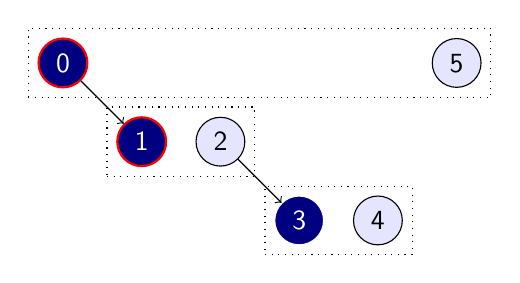
\begin{tikzpicture}
    \node[doc,active,fully](0) at (0,0){0};
    \node[doc,jshactive,fully](1) at (1,-1){1};
    \node[doc](2) at (2,-1){2};
    \node[doc,active](3) at (3,-2){3};
    \node[doc](4) at (4,-2){4};
    \node[doc](5) at (5,0){5};
    \node[draw,dotted,fit=(0)(5)] {};
    \node[draw,dotted,fit=(1)(2)] {};
    \node[draw,dotted,fit=(3)(4)] {};
    \draw[->](0)--(1);
    \draw[->](2)--(3);
  \end{tikzpicture}\]
  which moves forwards by $1$ to:
  \[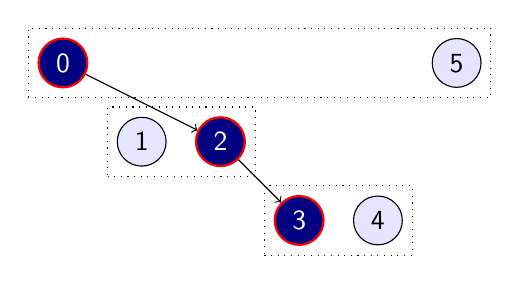
\begin{tikzpicture}
    \node[doc,active,fully](0) at (0,0){0};
    \node[doc](1) at (1,-1){1};
    \node[doc,jshactive,fully](2) at (2,-1){2};
    \node[doc,active,fully](3) at (3,-2){3};
    \node[doc](4) at (4,-2){4};
    \node[doc](5) at (5,0){5};
    \node[draw,dotted,fit=(0)(5)] {};
    \node[draw,dotted,fit=(1)(2)] {};
    \node[draw,dotted,fit=(3)(4)] {};
    \draw[->](0)--(2);
    \draw[->](2)--(3);
  \end{tikzpicture}\]
  which in turn moves forwards by $1$ to:
  \[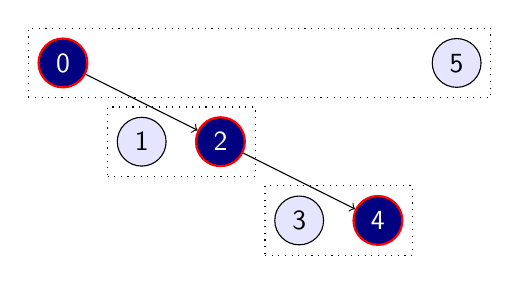
\begin{tikzpicture}
    \node[doc,active,fully](0) at (0,0){0};
    \node[doc](1) at (1,-1){1};
    \node[doc,active,fully](2) at (2,-1){2};
    \node[doc](3) at (3,-2){3};
    \node[doc,jshactive,fully](4) at (4,-2){4};
    \node[doc](5) at (5,0){5};
    \node[draw,dotted,fit=(0)(5)] {};
    \node[draw,dotted,fit=(1)(2)] {};
    \node[draw,dotted,fit=(3)(4)] {};
    \draw[->](0)--(2);
    \draw[->](2)--(4);
  \end{tikzpicture}\]
  but $H$ goes forward by $2$ to:
  \[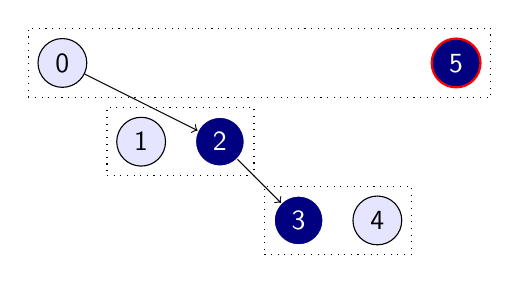
\begin{tikzpicture}
    \node[doc](0) at (0,0){0};
    \node[doc](1) at (1,-1){1};
    \node[doc,active](2) at (2,-1){2};
    \node[doc,active](3) at (3,-2){3};
    \node[doc](4) at (4,-2){4};
    \node[doc,jshactive,fully](5) at (5,0){5};
    \node[draw,dotted,fit=(0)(5)] {};
    \node[draw,dotted,fit=(1)(2)] {};
    \node[draw,dotted,fit=(3)(4)] {};
    \draw[->](0)--(2);
    \draw[->](2)--(3);
  \end{tikzpicture}\]
\end{counterexample}
The problem this time is that the definition of `joint session history' only includes
the fully active documents, not all active documents.

\begin{patch}
Define:
\begin{itemize}
\item the \emph{joint session future} is $\{ \bDoc \mid \exists \aDoc \in \Active \st \aDoc \ltSess \bDoc \}$, and
\item the \emph{joint session past} is $\{ \bDoc \mid \exists \aDoc \in \Active \st \aDoc \gtSess \bDoc \}$.
\end{itemize}
\end{patch}


\begin{counterexample}
  Let $H$ be:
  %% \[\begin{tikzpicture}
  %%   \node[doc,active,fully](0) at (0,0){0};
  %%   \node[doc](1) at (1,-1){1};
  %%   \node[doc](2) at (2,-2){2};
  %%   \node[doc,active,fully](3) at (3,-2){3};
  %%   \node[doc,jshactive,fully](4) at (4,-1){4};
  %%   \node[draw,dotted,fit=(0)]{};
  %%   \node[draw,dotted,fit=(1)(4)]{};
  %%   \node[draw,dotted,fit=(2)(3)]{};
  %%   \draw[->](0)--(4);
  %%   \draw[->](0)to[out=-20,in=120](3);
  %% \end{tikzpicture}\]
  %% which traverses the history by $-1$ to:
  \[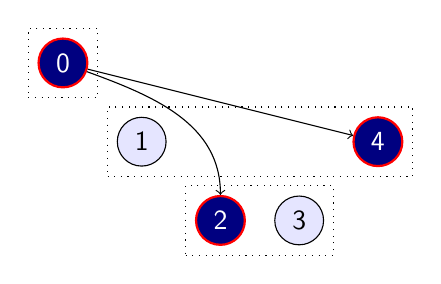
\begin{tikzpicture}
    \node[doc,active,fully](0) at (0,0){0};
    \node[doc](1) at (1,-1){1};
    \node[doc,jshactive,fully](2) at (2,-2){2};
    \node[doc](3) at (3,-2){3};
    \node[doc,active,fully](4) at (4,-1){4};
    \node[draw,dotted,fit=(0)]{};
    \node[draw,dotted,fit=(1)(4)]{};
    \node[draw,dotted,fit=(2)(3)]{};
    \draw[->](0)--(4);
    \draw[->](0)to[out=-20,in=90](2);
  \end{tikzpicture}\]
  which traverses the history by $-1$ to:
  \[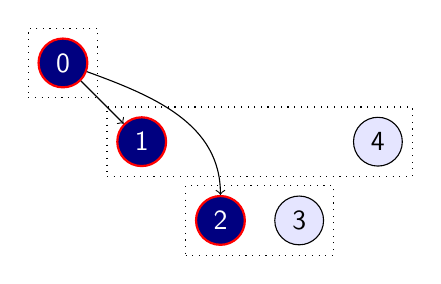
\begin{tikzpicture}
    \node[doc,active,fully](0) at (0,0){0};
    \node[doc,jshactive,fully](1) at (1,-1){1};
    \node[doc,active,fully](2) at (2,-2){2};
    \node[doc](3) at (3,-2){3};
    \node[doc](4) at (4,-1){4};
    \node[draw,dotted,fit=(0)]{};
    \node[draw,dotted,fit=(1)(4)]{};
    \node[draw,dotted,fit=(2)(3)]{};
    \draw[->](0)--(1);
    \draw[->](0)to[out=-20,in=90](2);
  \end{tikzpicture}\]
  which traverses the history by $1$ to:
  \[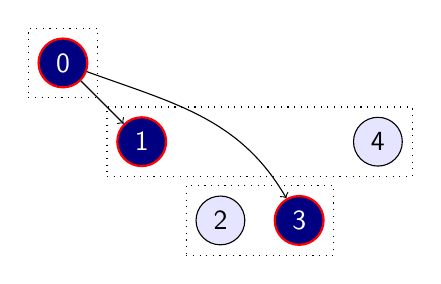
\begin{tikzpicture}
    \node[doc,active,fully](0) at (0,0){0};
    \node[doc,active,fully](1) at (1,-1){1};
    \node[doc](2) at (2,-2){2};
    \node[doc,jshactive,fully](3) at (3,-2){3};
    \node[doc](4) at (4,-1){4};
    \node[draw,dotted,fit=(0)]{};
    \node[draw,dotted,fit=(1)(4)]{};
    \node[draw,dotted,fit=(2)(3)]{};
    \draw[->](0)--(1);
    \draw[->](0)to[out=-20,in=120](3);
  \end{tikzpicture}\]
  %% which traverses the history by $1$ to:
  %% \[\begin{tikzpicture}
  %%   \node[doc,active,fully](0) at (0,0){0};
  %%   \node[doc](1) at (1,-1){1};
  %%   \node[doc](2) at (2,-2){2};
  %%   \node[doc,active,fully](3) at (3,-2){3};
  %%   \node[doc,jshactive,fully](4) at (4,-1){4};
  %%   \node[draw,dotted,fit=(0)]{};
  %%   \node[draw,dotted,fit=(1)(4)]{};
  %%   \node[draw,dotted,fit=(2)(3)]{};
  %%   \draw[->](0)--(4);
  %%   \draw[->](0)to[out=-20,in=120](3);
  %% \end{tikzpicture}\]
  which is not the same as $H$.
\end{counterexample}

[ASAJ: Not sure about this\dots]

\begin{patch}
Define \emph{$\aNH$ traverses the history from $\aDoc'$} when there is some $\aDoc$ such that:
\begin{itemize}
\item $\aDoc\ltSess\aDoc'$,
\item for any $\bDoc\ltSess\aDoc'$ we have $\bDoc\leChron\aDoc$, and
\item $\aNH$ traverses the history to $\aDoc$.
\end{itemize}
Define \emph{$\aNH$ traverses the history by $-\delta$ to $\aNH'$} when:
\begin{itemize}
\item the joint session past and active documents of $\aNH$ is $\aDoc_1 \gtChron \cdots \gtChron \aDoc_\delta \gtChron \cdots$,
\item there is some $\aNH=\aNH_0,\ldots,\aNH_\delta=\aNH'$, such that
\item $H_{i-1}$ traverses the history from $d_i$ in $H_i$ for each $1 \le i \le \delta$.
\end{itemize}
\end{patch}

\begin{goal}
  If $\aDoc$ in $\aNH$ navigates to $\aDoc'$ in $\aNH'$,
  and $\aNH'$ traverses the history by $-1$ to $\aNH''$,
  then $\FullyActive=\FullyActive''$.
\end{goal}

%% \begin{counterexample}
%%   \[\begin{tikzpicture}
%%     \node[doc,active,fully](0) at (0,0){0};
%%     \node[doc,jshactive,fully](1) at (1,-1){1};
%%     \node[doc](2) at (2,0){2};
%%     \node[draw,dotted,fit=(0)(2)] {};
%%     \node[draw,dotted,fit=(1)]{};
%%     \draw[->](0)--(1);
%%   \end{tikzpicture}\]
%%   navigates 1 to 3 in:
%%   \[\begin{tikzpicture}
%%     \node[doc,active,fully](0) at (0,0){0};
%%     \node[doc](1) at (1,-1){1};
%%     \node[doc](2) at (2,0){2};
%%     \node[doc,jshactive,fully](3) at (3,-1){3};
%%     \node[draw,dotted,fit=(0)(2)] {};
%%     \node[draw,dotted,fit=(1)(3)]{};
%%     \draw[->](0)--(3);
%%   \end{tikzpicture}\]
%%   which traverses the history by $-1$ to:
%%   \[\begin{tikzpicture}
%%     \node[doc](0) at (0,0){0};
%%     \node[doc](1) at (1,-1){1};
%%     \node[doc,jshactive,fully](2) at (2,0){2};
%%     \node[doc,active](3) at (3,-1){3};
%%     \node[draw,dotted,fit=(0)(2)] {};
%%     \node[draw,dotted,fit=(1)(3)]{};
%%     \draw[->](0)--(3);
%%   \end{tikzpicture}\]
%% \end{counterexample}

\section{Experiments}

[In this section various different navigation and traversal scenarios are tested in popular web browsers to see where they differ in behaviour from both the spec and each other.]

\begin{experiment}
  In this experiment Goal~\ref{goal:homomorphism} is tested.
  \begin{itemize}
    \item \emph{$\aNH$ traverses the history by $-4$ to $\aNH'$}
    \item \emph{$\aNH'$ traverses the history by $+4$ to $\aNH''$}
  \end{itemize}
  By Goal~\ref{goal:homomorphism}, these traversals should be the same thing as \emph{$\aNH$ traversing by $0$} which is a no-op; therefore, $\aNH = \aNH''$.

  Firefox:
  \begin{figure}[H]
    \raisebox{-.5\height}{
      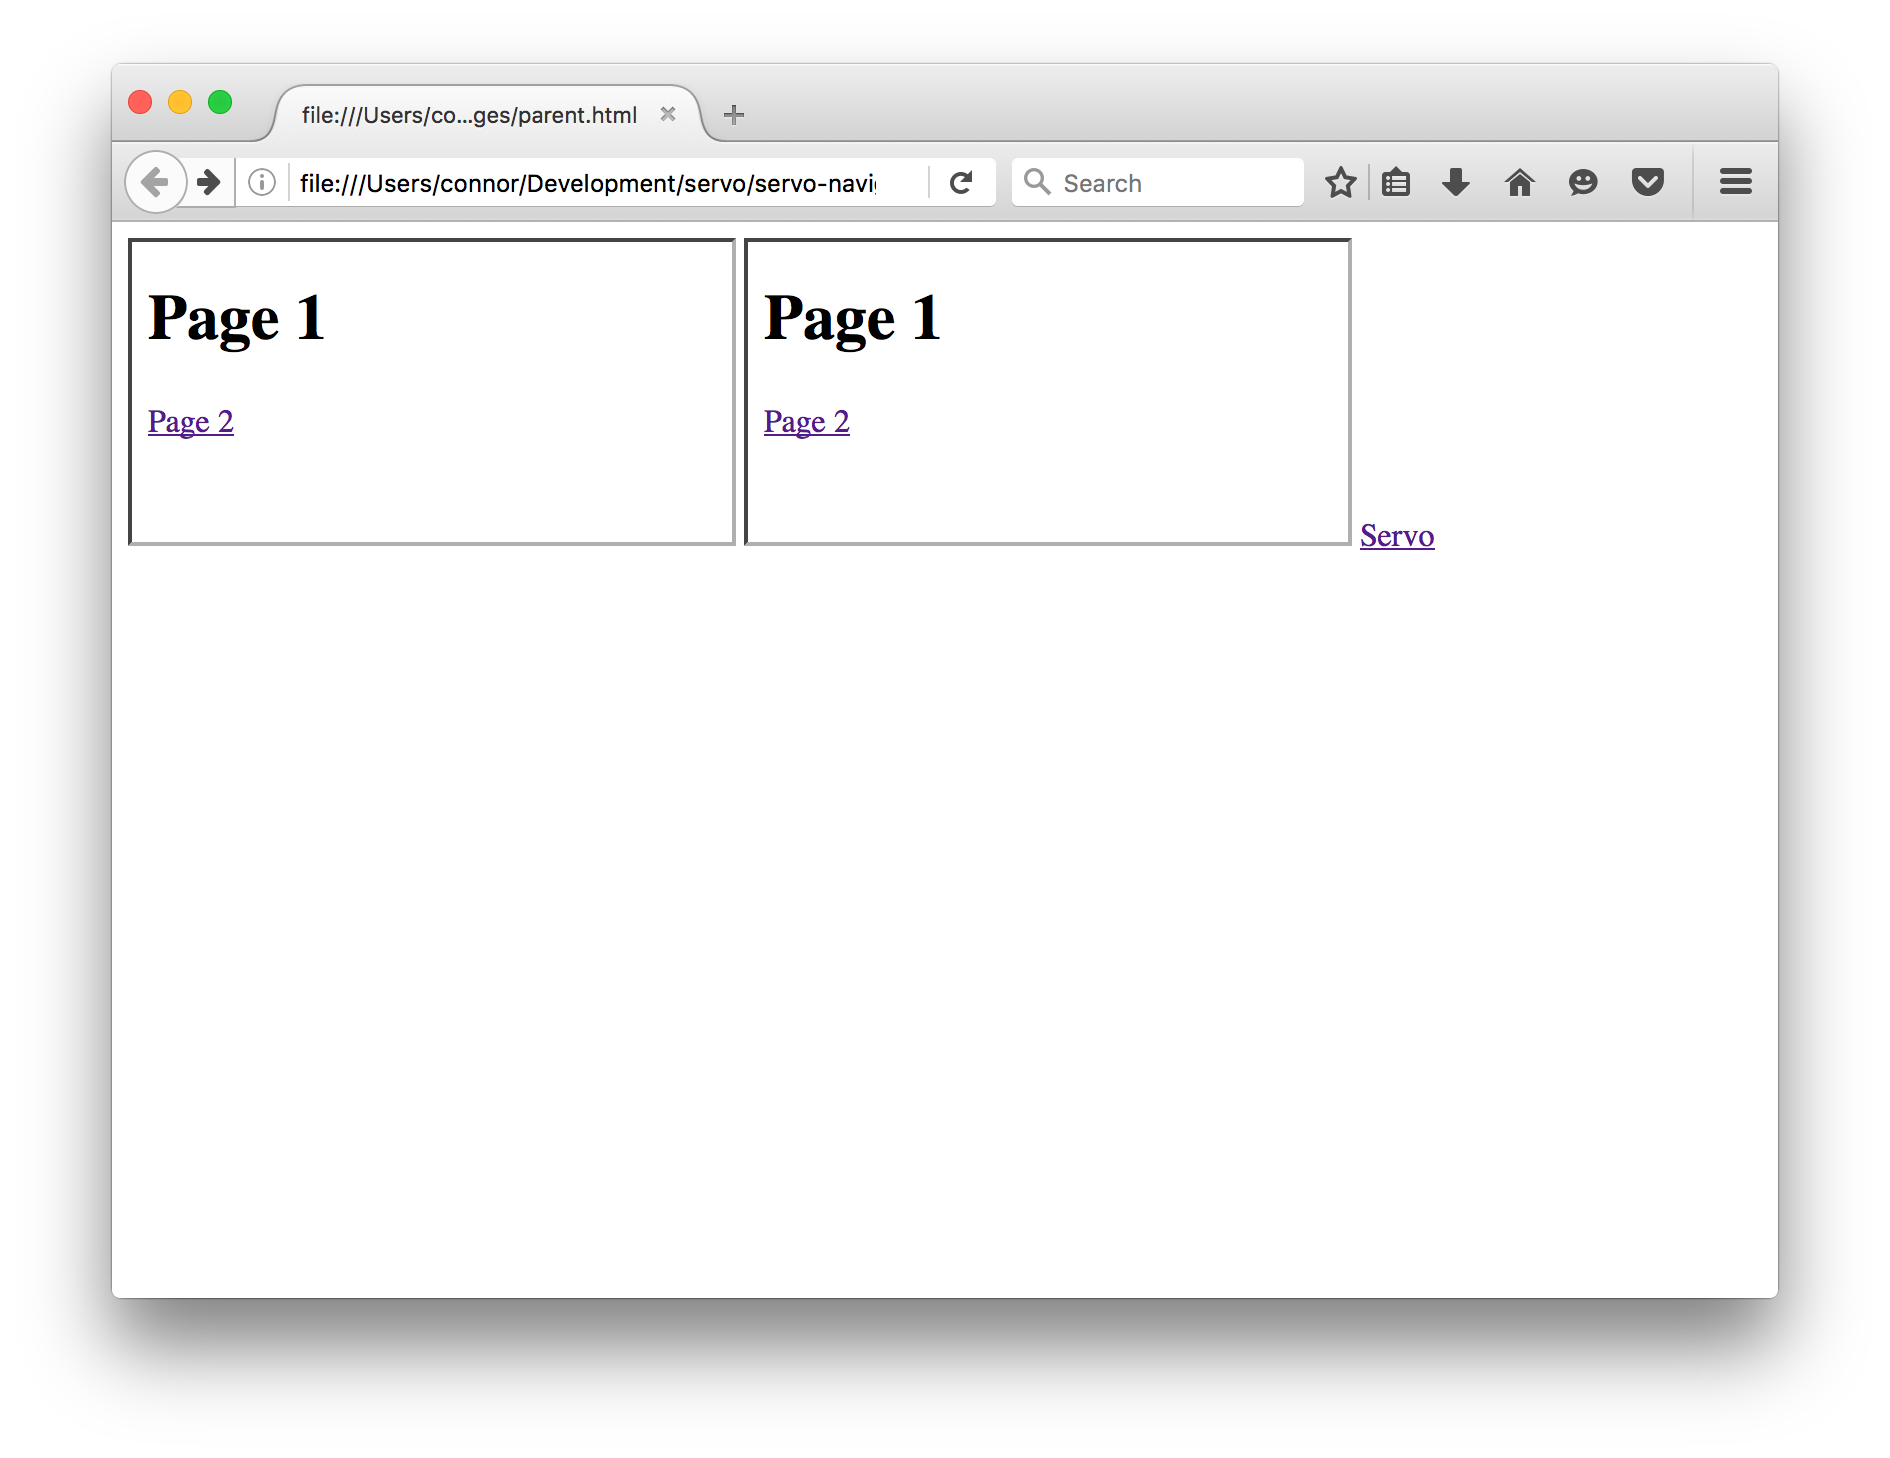
\includegraphics[width=.5\linewidth]{images/experiments/forwardback4/firefox/1.png}%
    }~\raisebox{-.5\height}{
      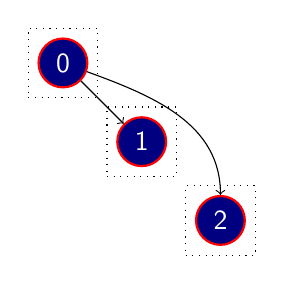
\begin{tikzpicture}
        \node[doc,active,fully](0) at (0,0){0};
        \node[doc,active,fully](1) at (1,-1){1};
        \node[doc,jshactive,fully](2) at (2,-2){2};
        \node[draw,dotted,fit=(0)]{};
        \node[draw,dotted,fit=(1)]{};
        \node[draw,dotted,fit=(2)]{};
        \draw[->](0)--(1);
        \draw[->](0)to[out=-20,in=90](2);
      \end{tikzpicture}
    }
    \caption{Initial State}
  \end{figure}

  Navigate document $1$ to Page 2:
  \begin{figure}[H]
    \raisebox{-.5\height}{
      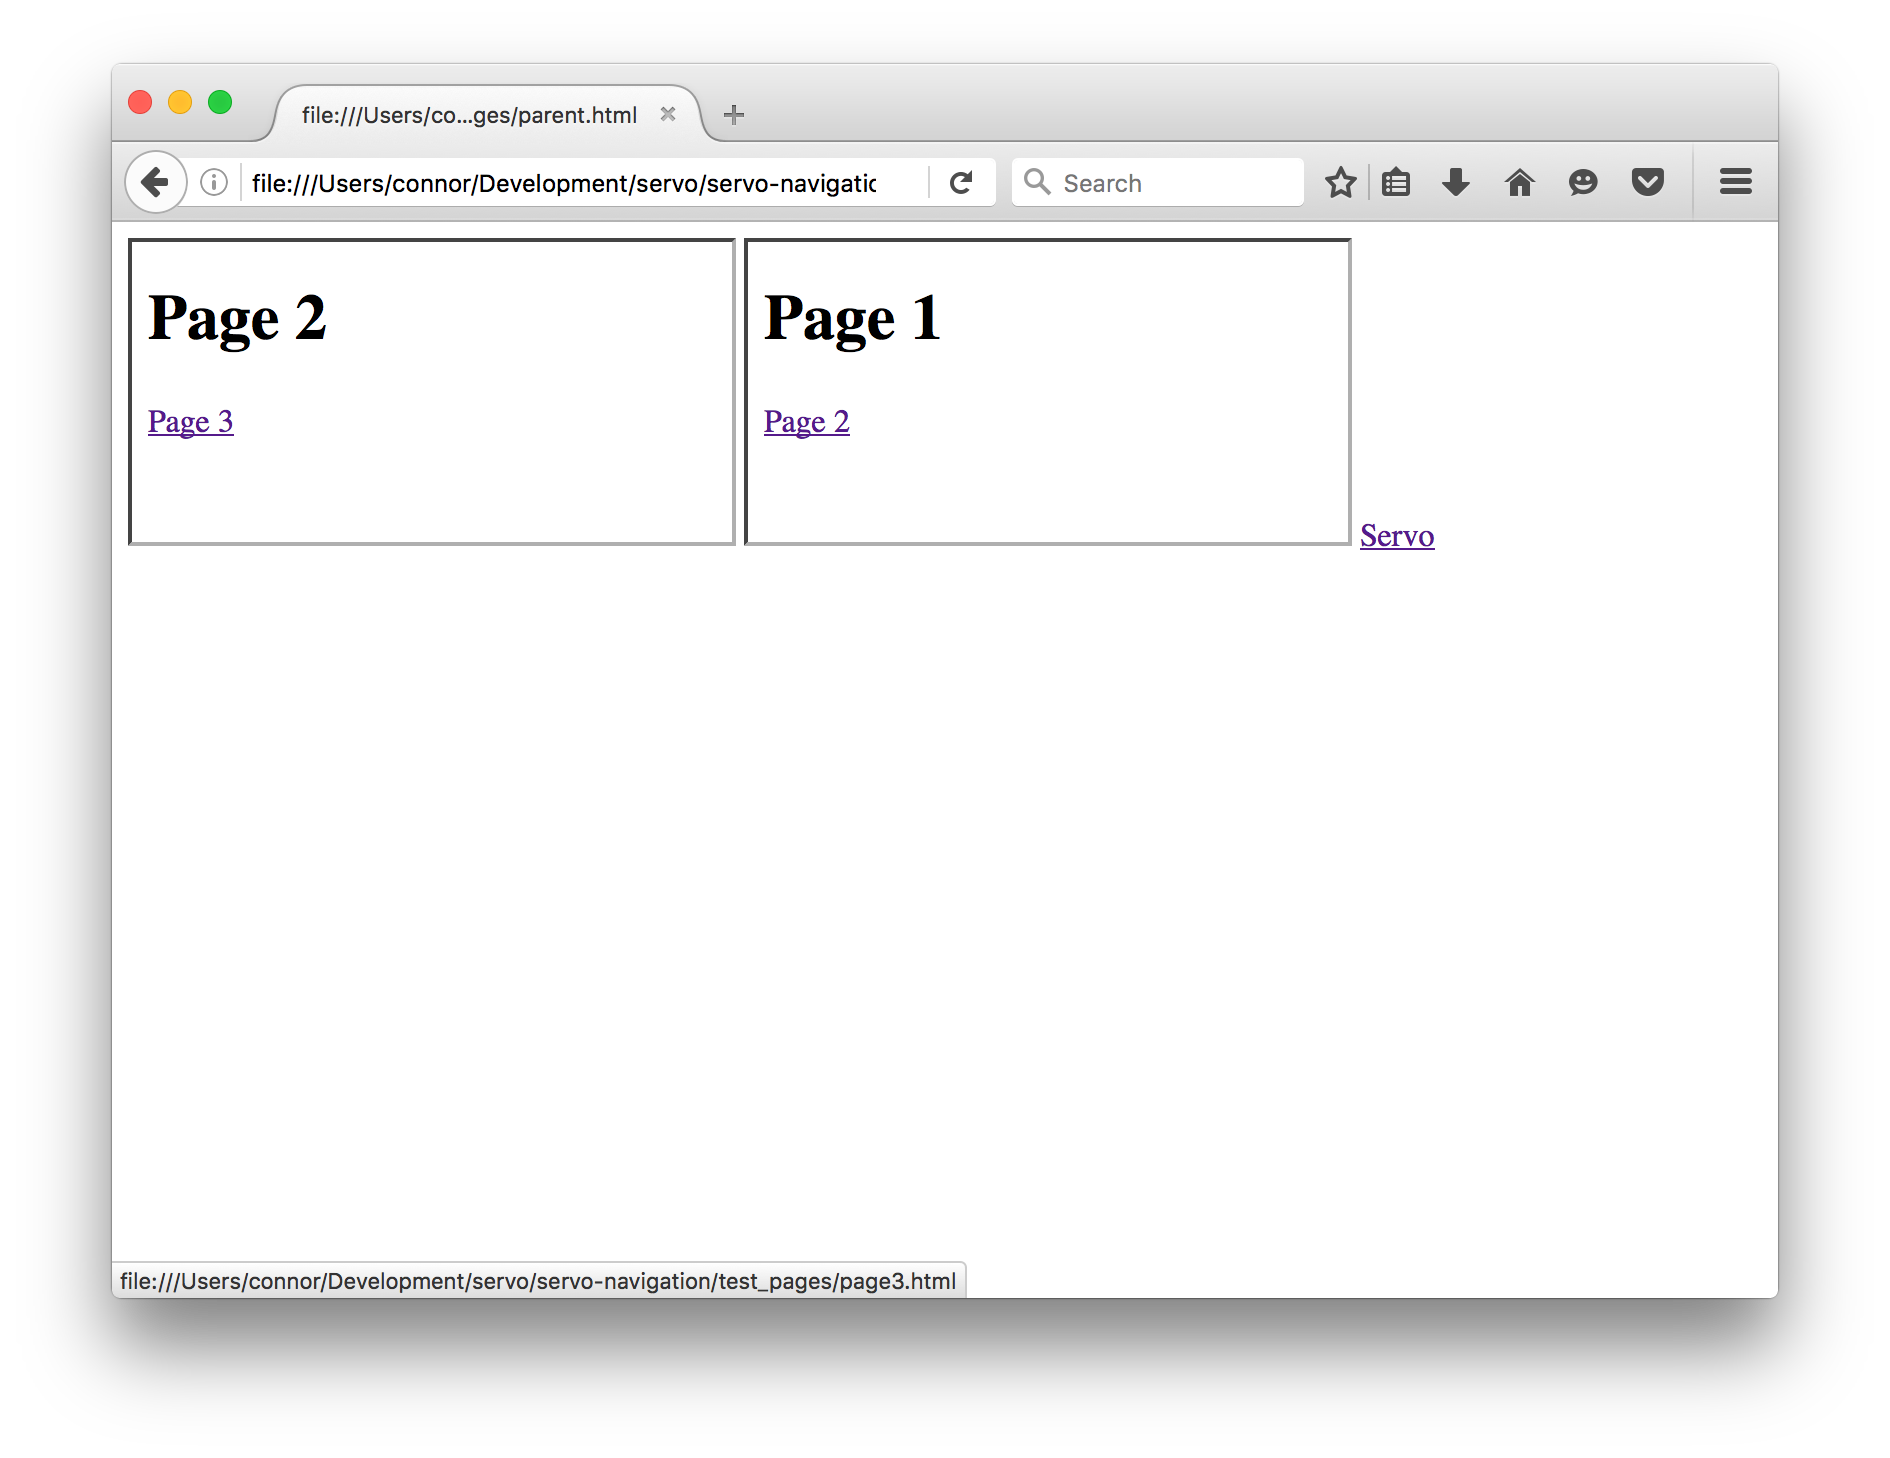
\includegraphics[width=.5\linewidth]{images/experiments/forwardback4/firefox/2.png}
    }~\raisebox{-.5\height}{
      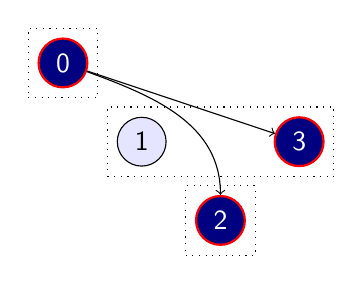
\begin{tikzpicture}
        \node[doc,active,fully](0) at (0,0){0};
        \node[doc](1) at (1,-1){1};
        \node[doc,active,fully](2) at (2,-2){2};
        \node[doc,jshactive,fully](3) at (3,-1){3};
        \node[draw,dotted,fit=(0)]{};
        \node[draw,dotted,fit=(1)(3)]{};
        \node[draw,dotted,fit=(2)]{};
        \draw[->](0)--(3);
        \draw[->](0)to[out=-20,in=90](2);
      \end{tikzpicture}
    }
    \caption{Navigate document $1$ to Page 2.}
  \end{figure}

  Navigate document $3$ to Page 3:
  \begin{figure}[H]
    \raisebox{-.5\height}{
      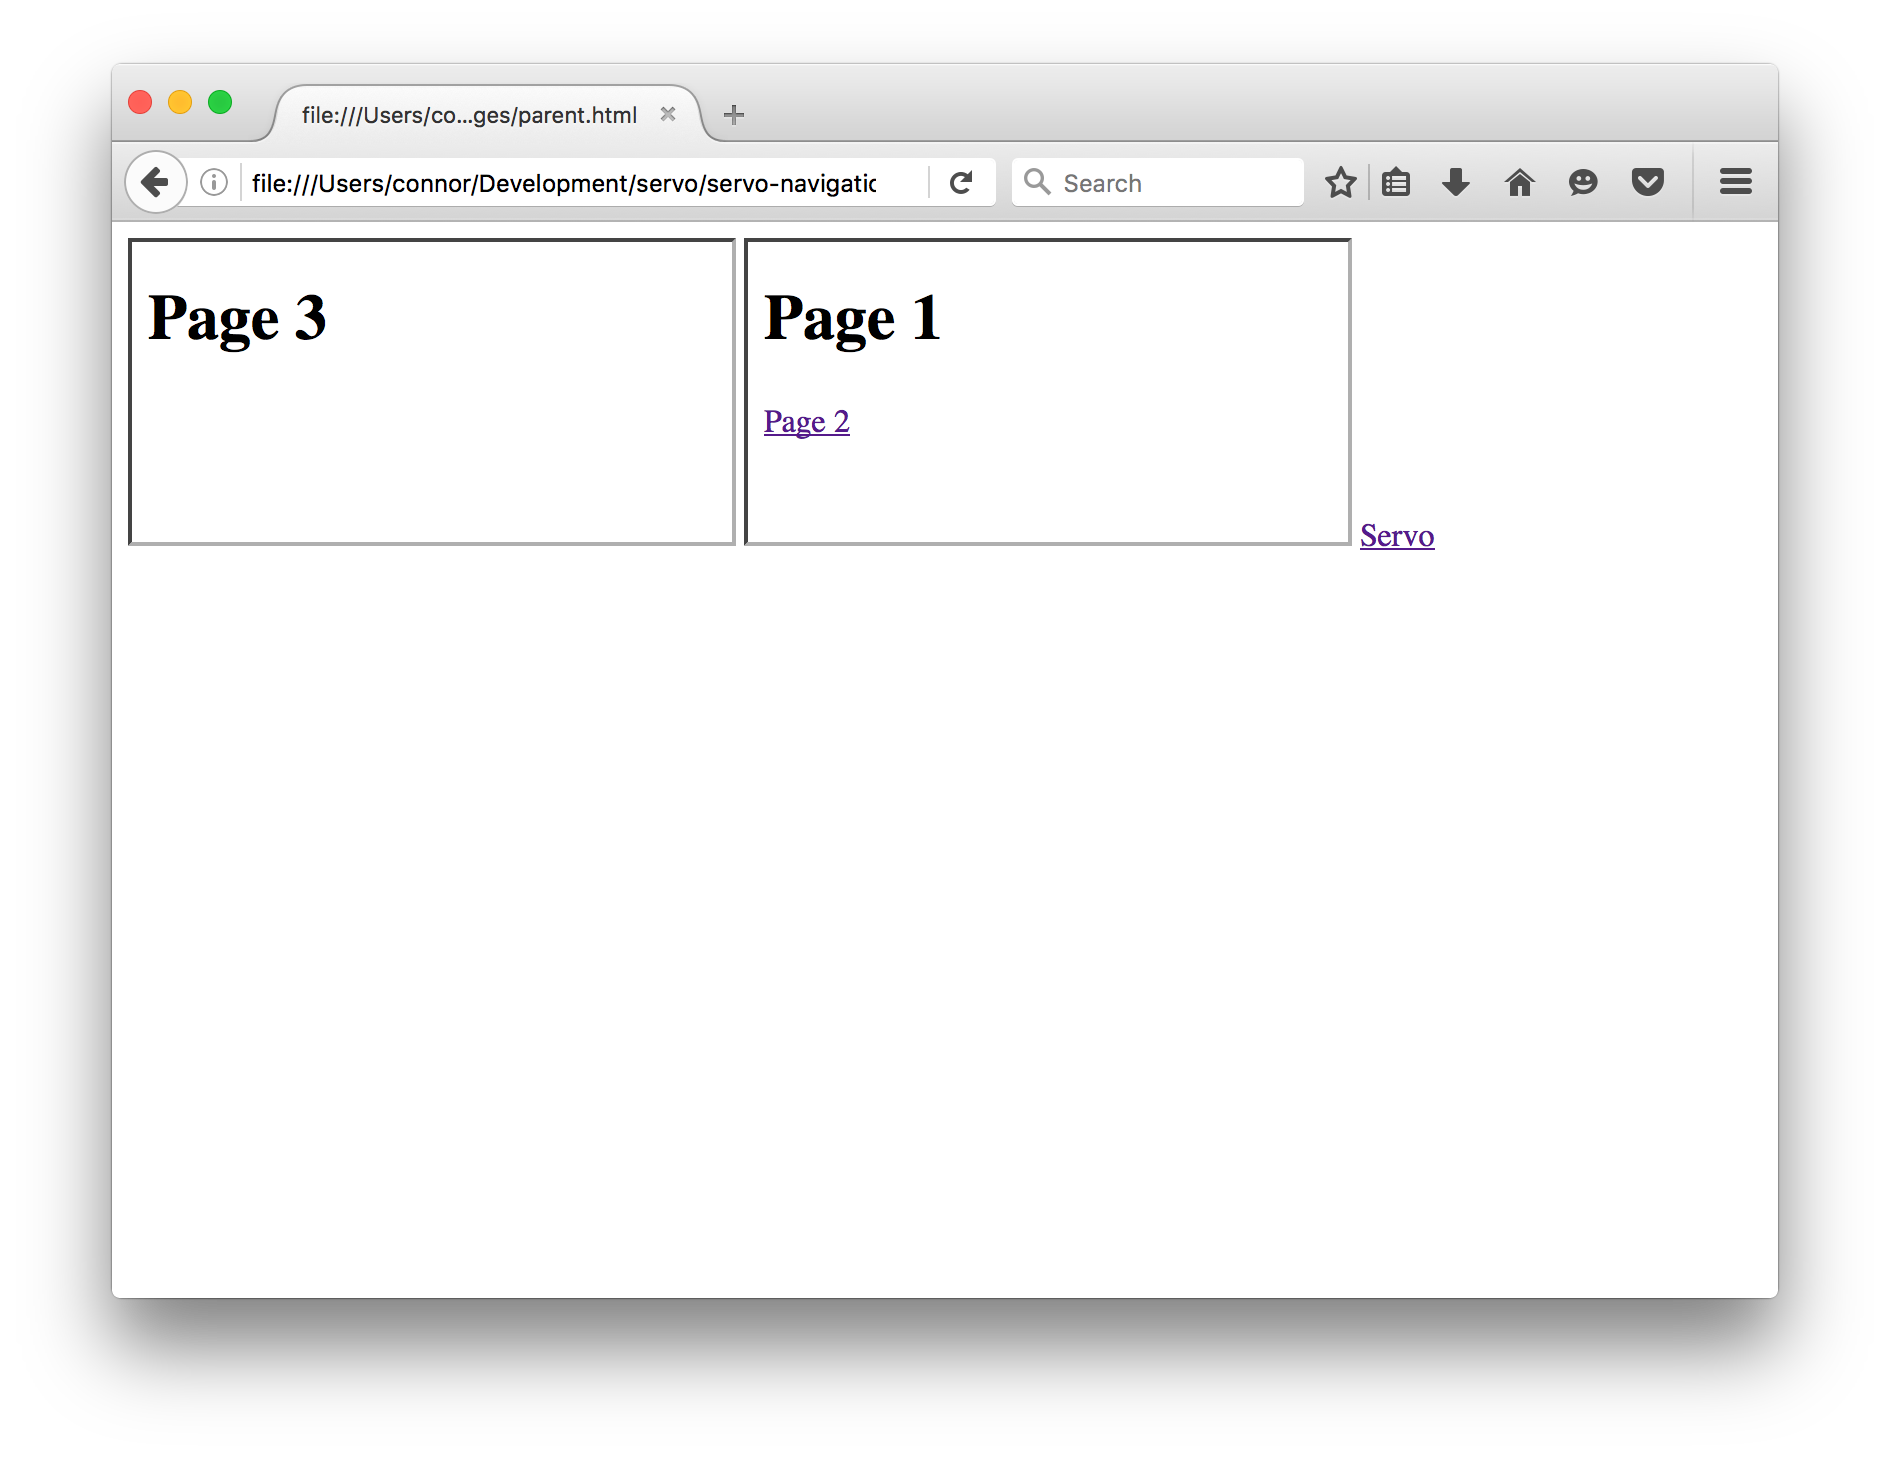
\includegraphics[width=.5\linewidth]{images/experiments/forwardback4/firefox/3.png}
    }~\raisebox{-.5\height}{
      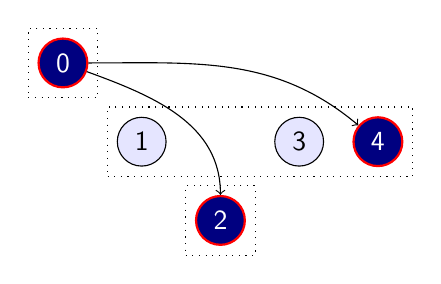
\begin{tikzpicture}
        \node[doc,active,fully](0) at (0,0){0};
        \node[doc](1) at (1,-1){1};
        \node[doc,active,fully](2) at (2,-2){2};
        \node[doc](3) at (3,-1){3};
        \node[doc,jshactive,fully](4) at (4,-1){4};
        \node[draw,dotted,fit=(0)]{};
        \node[draw,dotted,fit=(1)(4)]{};
        \node[draw,dotted,fit=(2)]{};
        \draw[->](0)to[out=0,in=140](4);
        \draw[->](0)to[out=-20,in=90](2);
      \end{tikzpicture}
    }
    \caption{Navigate document $3$ to Page 3.}
  \end{figure}

  Navigate document $2$ to Page 2:
  \begin{figure}[H]
    \raisebox{-.5\height}{
      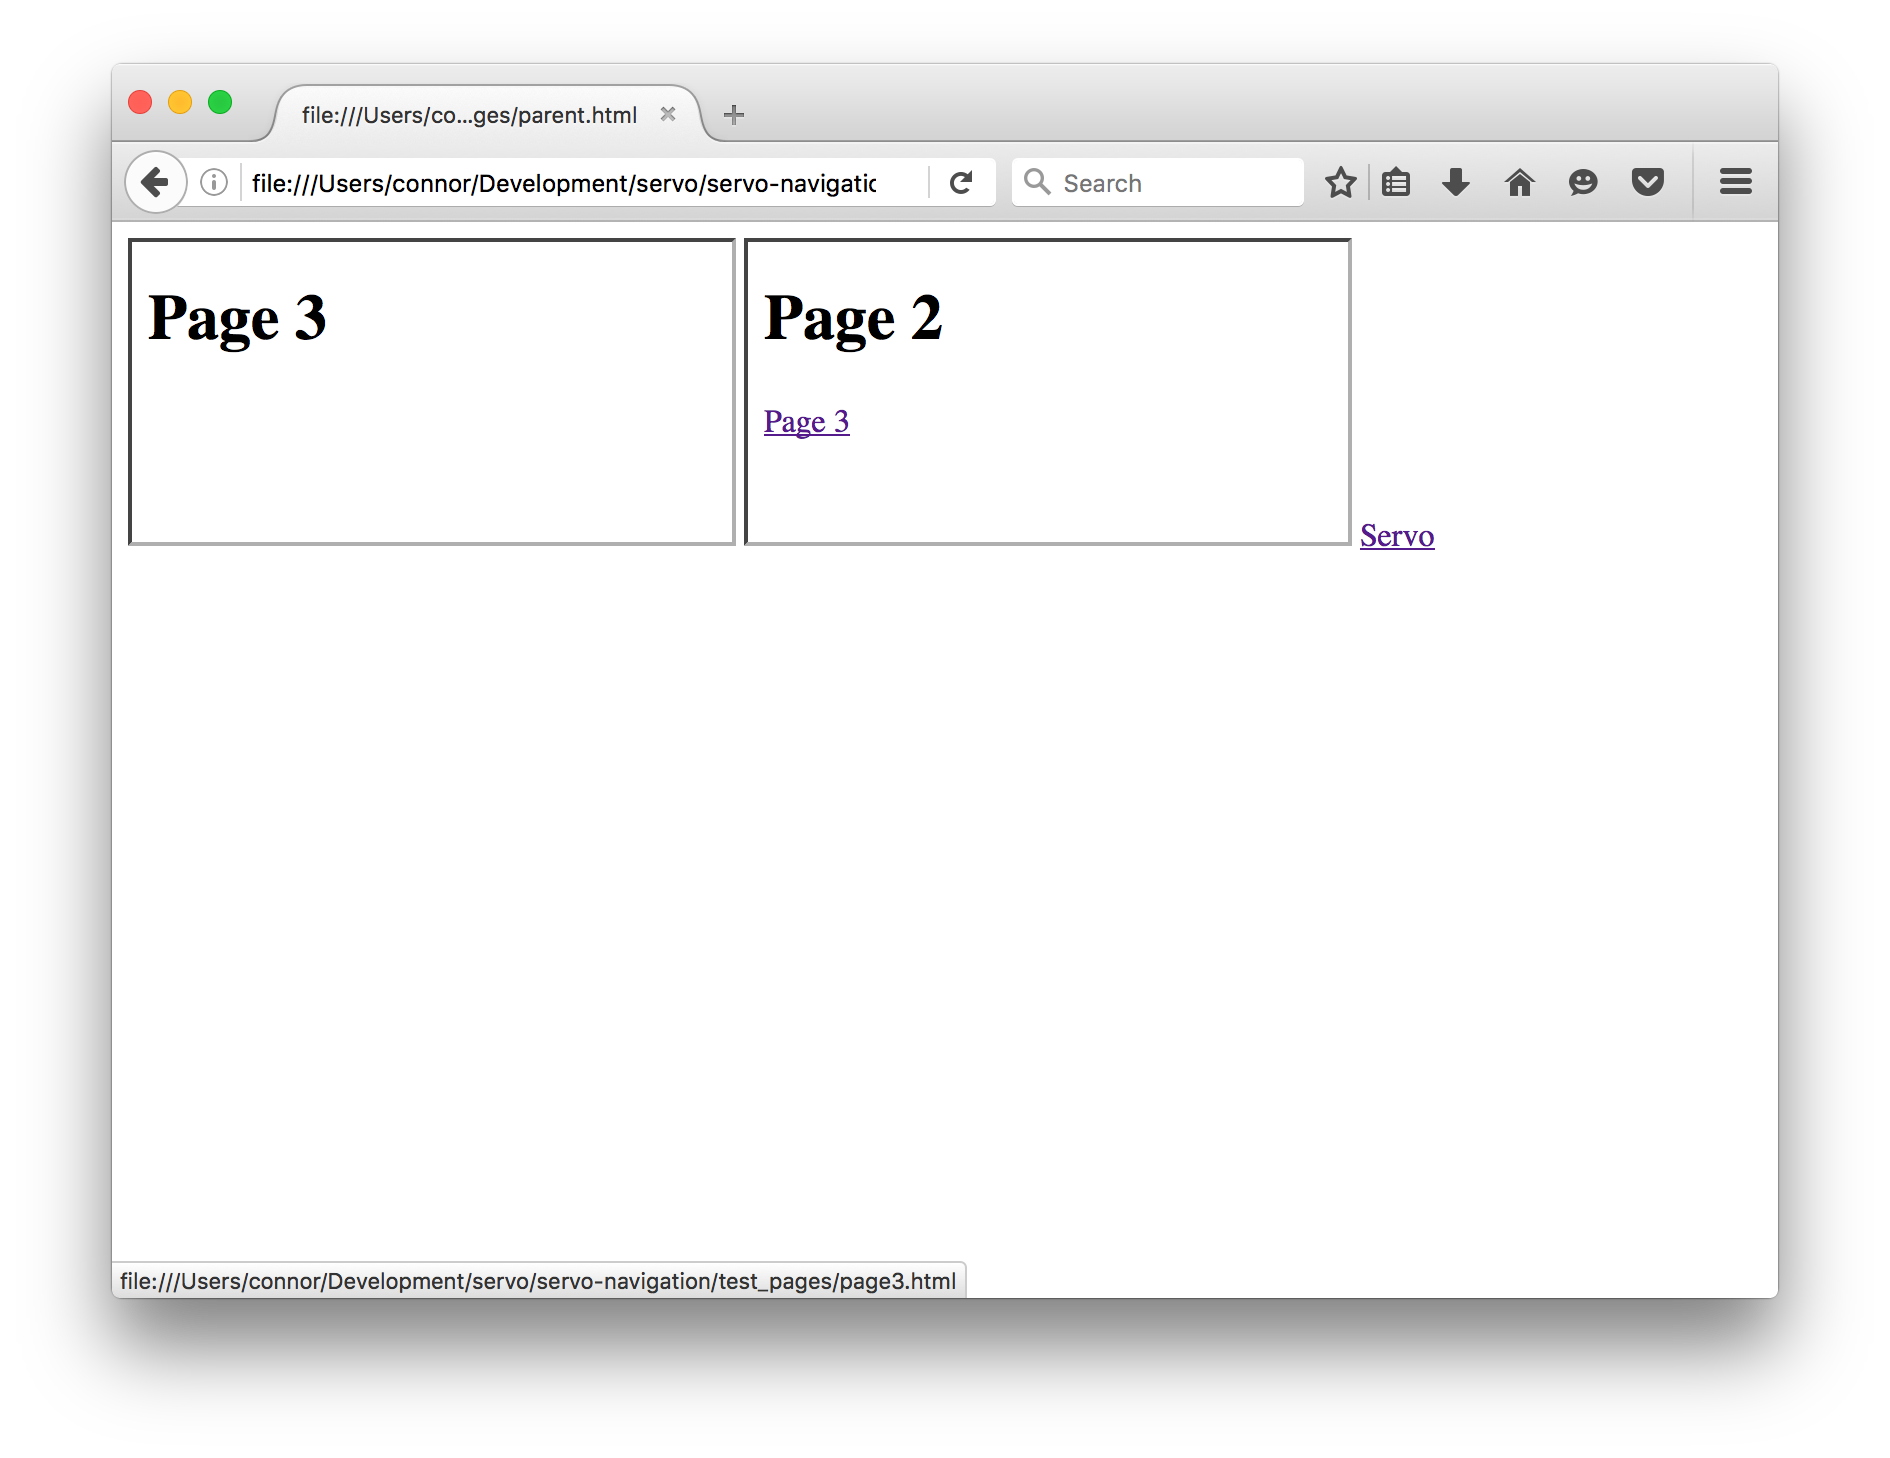
\includegraphics[width=.5\linewidth]{images/experiments/forwardback4/firefox/4.png}
    }~\raisebox{-.5\height}{
      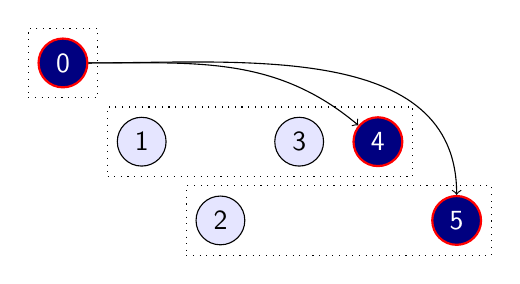
\begin{tikzpicture}
        \node[doc,active,fully](0) at (0,0){0};
        \node[doc](1) at (1,-1){1};
        \node[doc](2) at (2,-2){2};
        \node[doc](3) at (3,-1){3};
        \node[doc,active,fully](4) at (4,-1){4};
        \node[doc,jshactive,fully](5) at (5,-2){5};
        \node[draw,dotted,fit=(0)]{};
        \node[draw,dotted,fit=(1)(4)]{};
        \node[draw,dotted,fit=(2)(5)]{};
        \draw[->](0)to[out=0,in=140](4);
        \draw[->](0)to[out=0,in=90](5);
      \end{tikzpicture}
    }
    \caption{Navigate document $2$ to Page 2.}
  \end{figure}

  Navigate document $5$ to Page 3:
  \begin{figure}[H]
    \raisebox{-.5\height}{
      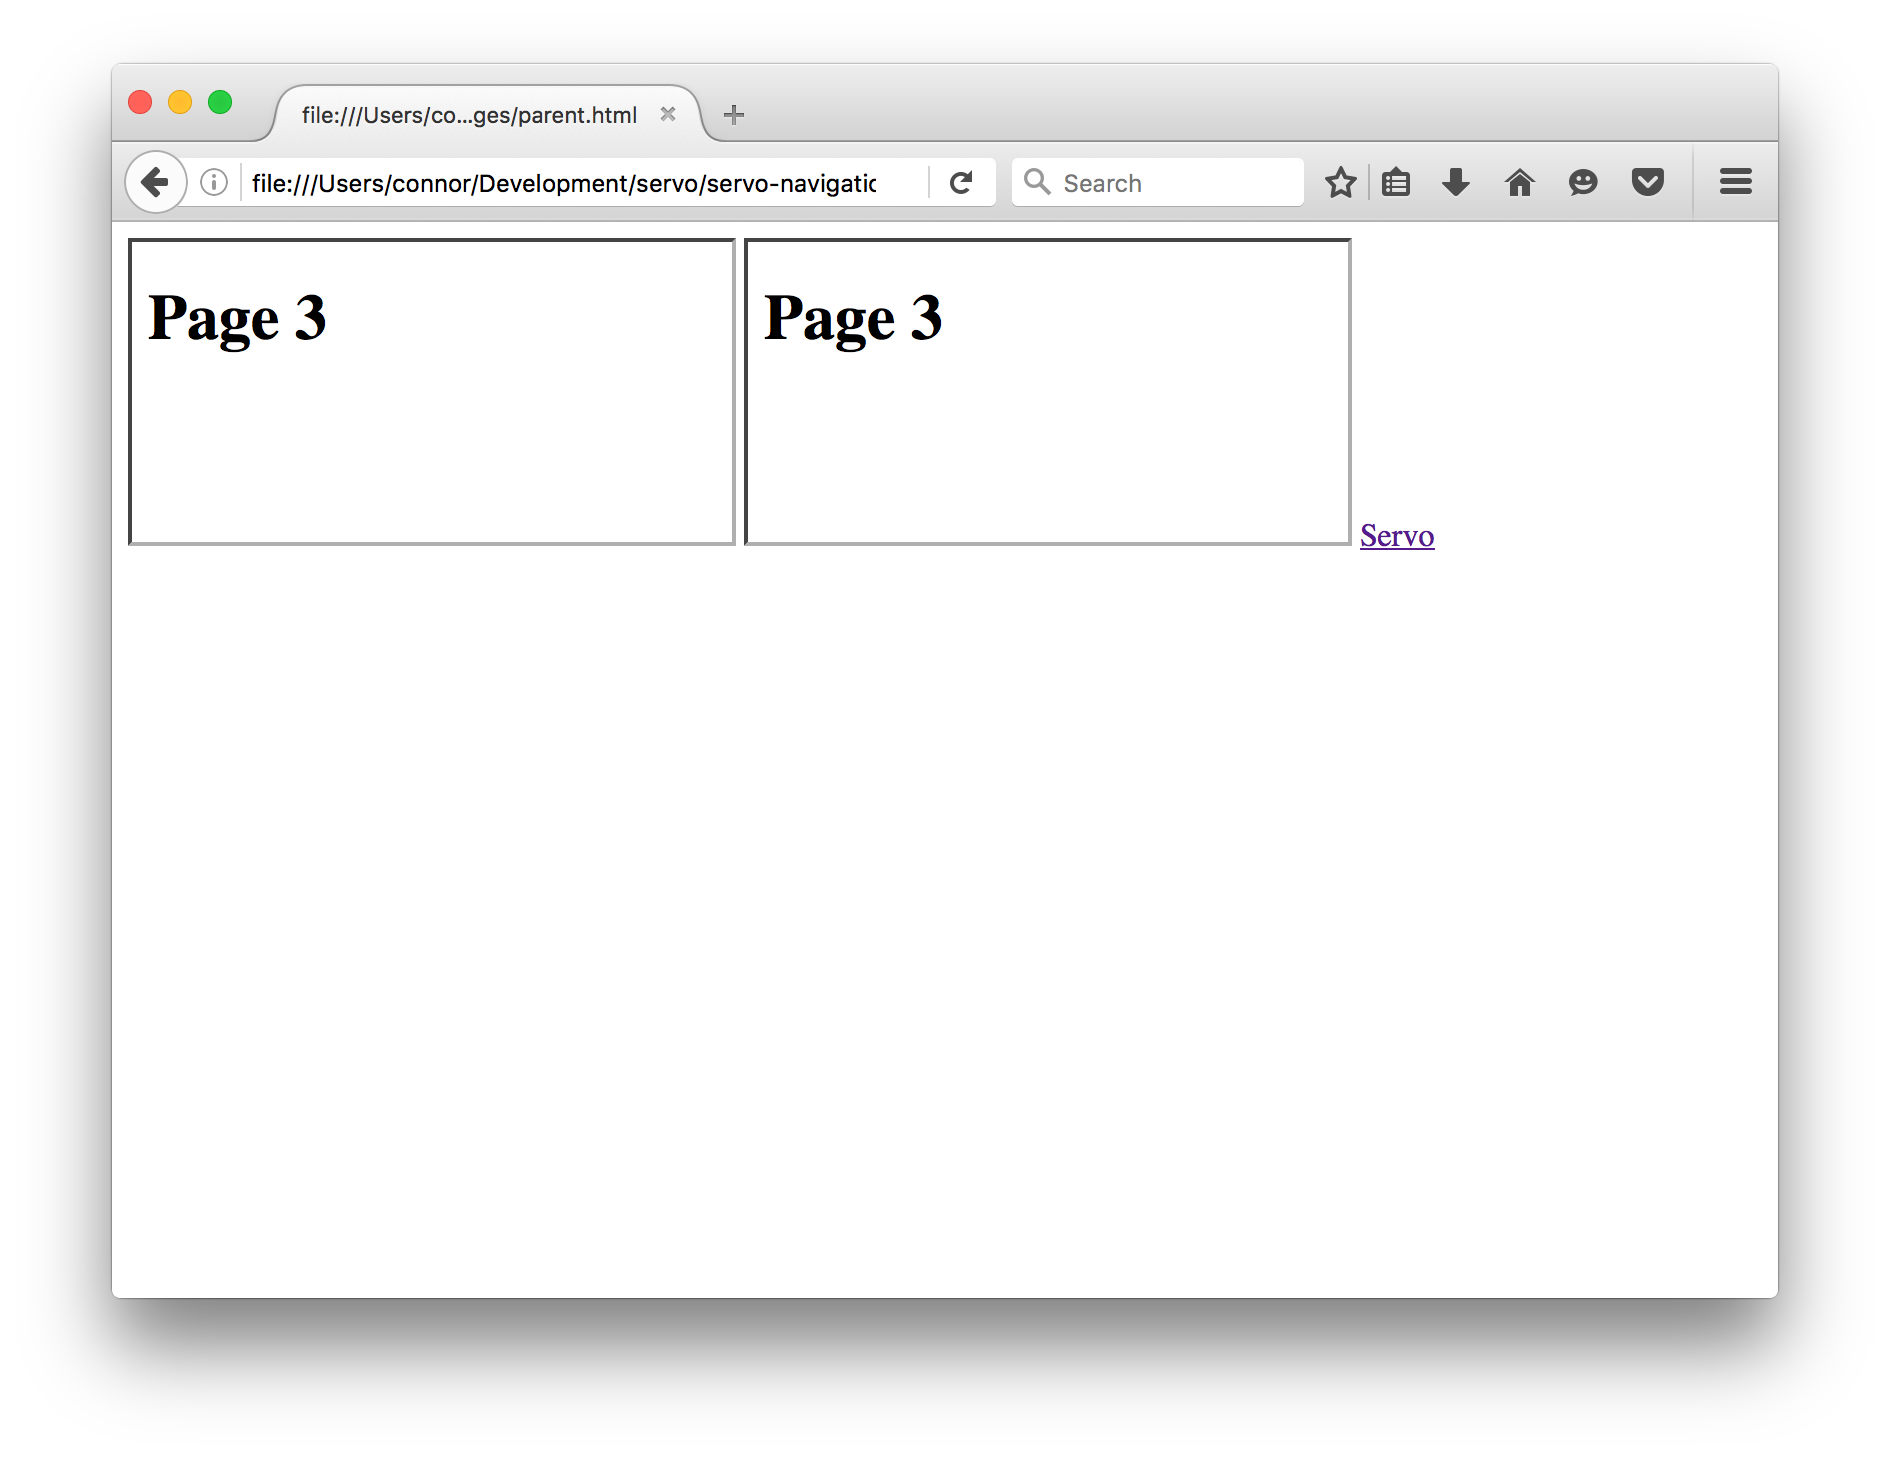
\includegraphics[width=.5\linewidth]{images/experiments/forwardback4/firefox/5.png}
    }~\raisebox{-.5\height}{
      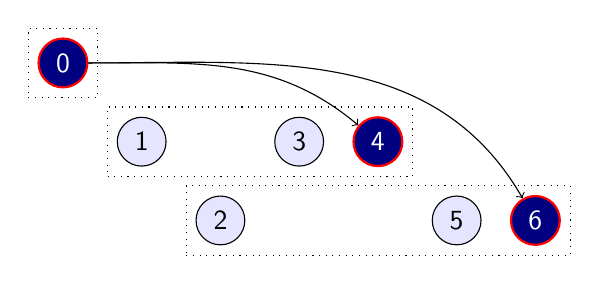
\begin{tikzpicture}
        \node[doc,active,fully](0) at (0,0){0};
        \node[doc](1) at (1,-1){1};
        \node[doc](2) at (2,-2){2};
        \node[doc](3) at (3,-1){3};
        \node[doc,active,fully](4) at (4,-1){4};
        \node[doc](5) at (5,-2){5};
        \node[doc,jshactive,fully](6) at (6,-2){6};
        \node[draw,dotted,fit=(0)]{};
        \node[draw,dotted,fit=(1)(4)]{};
        \node[draw,dotted,fit=(2)(6)]{};
        \draw[->](0)to[out=0,in=140](4);
        \draw[->](0)to[out=0,in=120](6);
      \end{tikzpicture}
    }
    \caption{Navigate document $5$ to Page 3.}
  \end{figure}

  \emph{$\aNH$ traverses the history by $-4$ to $\aNH'$}:
  \begin{figure}[H]
    \raisebox{-.5\height}{
      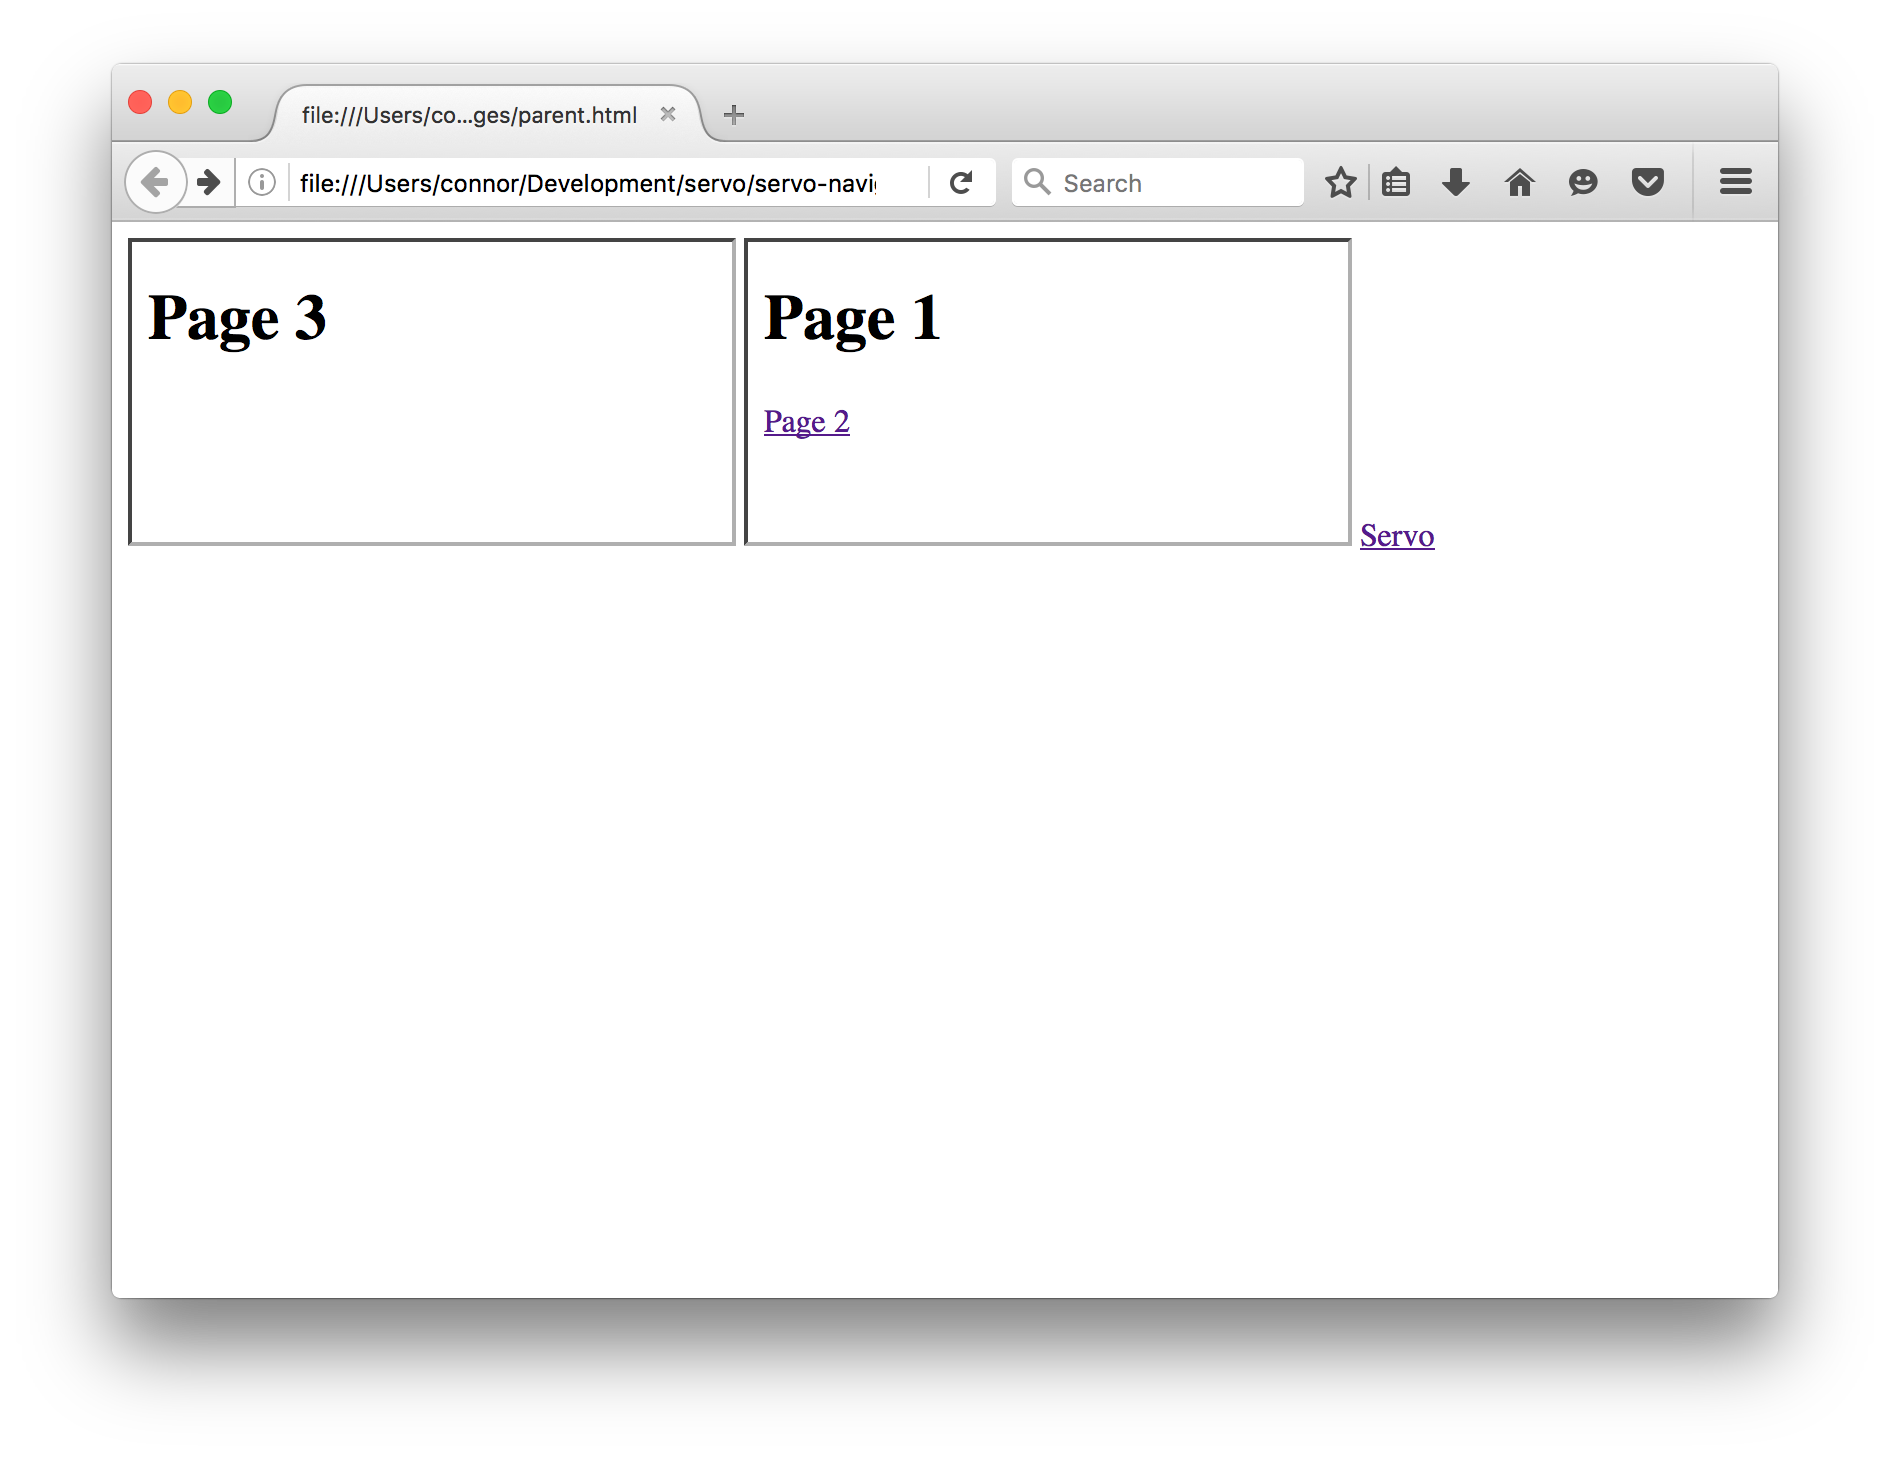
\includegraphics[width=.5\linewidth]{images/experiments/forwardback4/firefox/6.png}
    }~\raisebox{-.5\height}{
      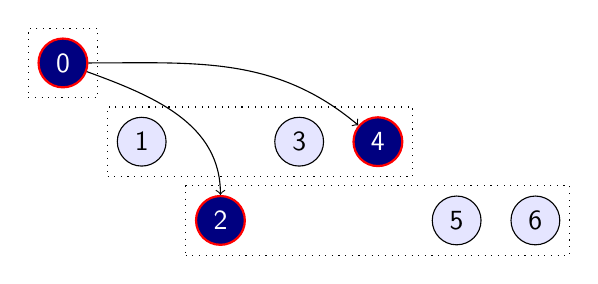
\begin{tikzpicture}
        \node[doc,active,fully](0) at (0,0){0};
        \node[doc](1) at (1,-1){1};
        \node[doc,jshactive,fully](2) at (2,-2){2};
        \node[doc](3) at (3,-1){3};
        \node[doc,active,fully](4) at (4,-1){4};
        \node[doc](5) at (5,-2){5};
        \node[doc](6) at (6,-2){6};
        \node[draw,dotted,fit=(0)]{};
        \node[draw,dotted,fit=(1)(4)]{};
        \node[draw,dotted,fit=(2)(6)]{};
        \draw[->](0)to[out=0,in=140](4);
        \draw[->](0)to[out=-20,in=90](2);
      \end{tikzpicture}
    }
    \caption{Traversal by $-4$.}
    \label{fig:traverseback4}
  \end{figure}

  This state is obviously wrong, as document $4$ should have traversed to document $1$.
  This is similar to counterexample~\ref{counterexample:homomorphism1}.

  \emph{$\aNH'$ traverses the history by $4$ to $\aNH''$}:
  \begin{figure}[H]
    \raisebox{-.5\height}{
      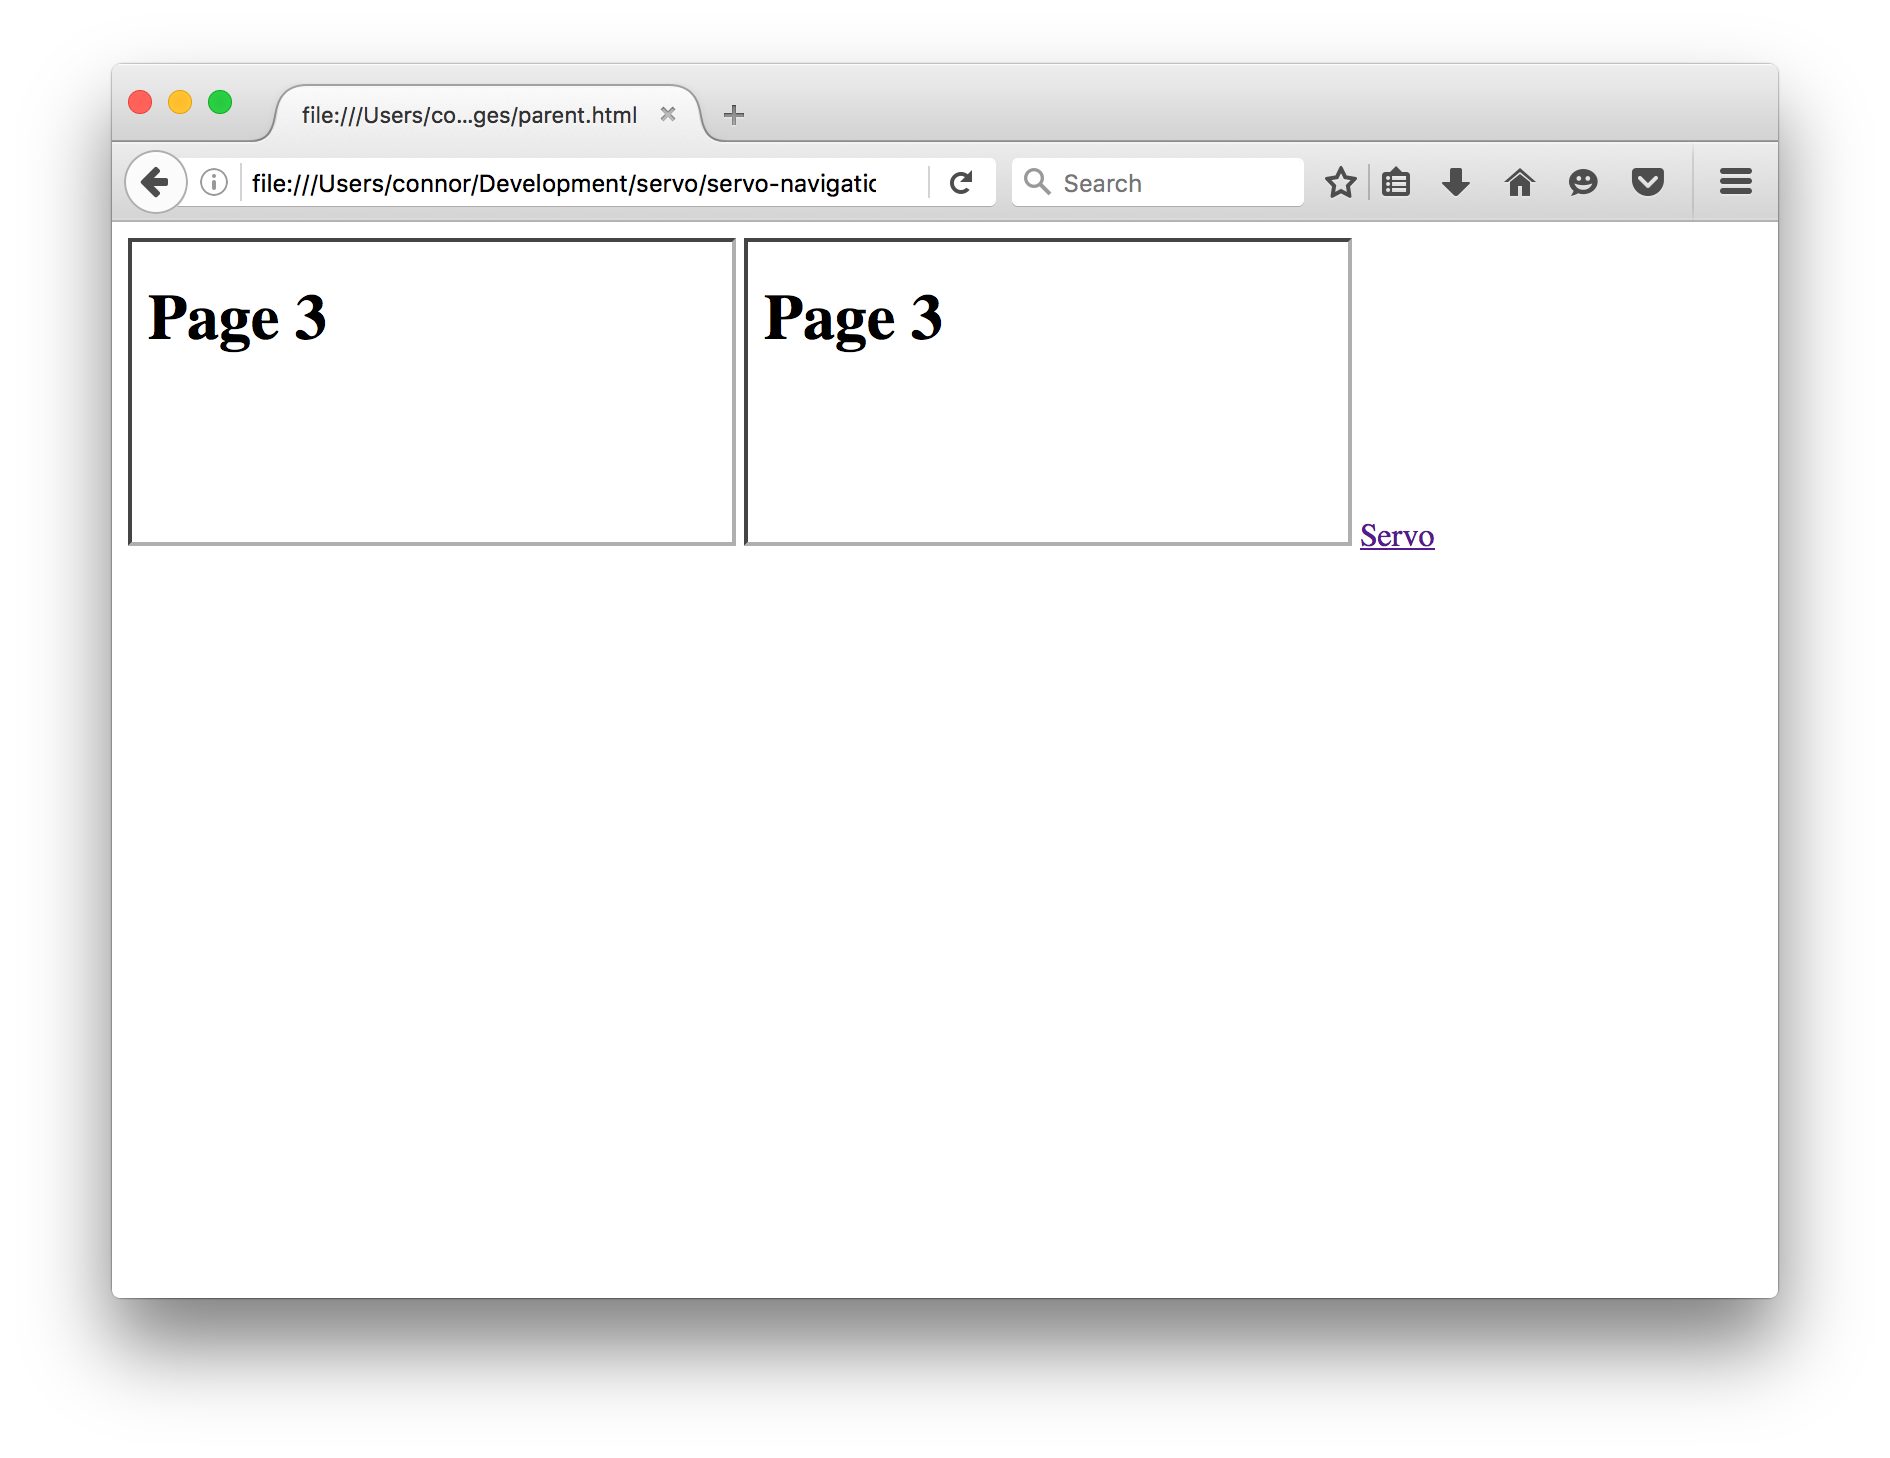
\includegraphics[width=.5\linewidth]{images/experiments/forwardback4/firefox/7.png}
    }~\raisebox{-.5\height}{
      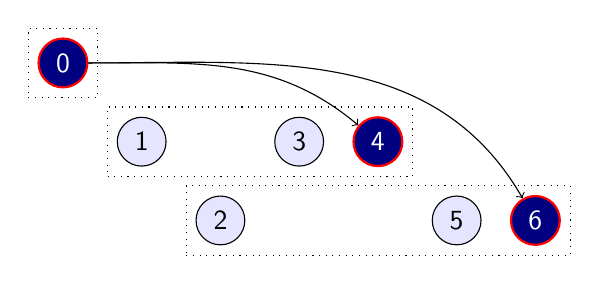
\begin{tikzpicture}
        \node[doc,active,fully](0) at (0,0){0};
        \node[doc](1) at (1,-1){1};
        \node[doc](2) at (2,-2){2};
        \node[doc](3) at (3,-1){3};
        \node[doc,active,fully](4) at (4,-1){4};
        \node[doc](5) at (5,-2){5};
        \node[doc,jshactive,fully](6) at (6,-2){6};
        \node[draw,dotted,fit=(0)]{};
        \node[draw,dotted,fit=(1)(4)]{};
        \node[draw,dotted,fit=(2)(6)]{};
        \draw[->](0)to[out=0,in=140](4);
        \draw[->](0)to[out=0,in=120](6);
      \end{tikzpicture}
    }
    \caption{Traversal by $4$.}
  \end{figure}

  While this result does satisfy Goal~\ref{goal:homomorphism}, there are still some issues:
  \begin{itemize}
    \item Figure~\ref{fig:traverseback4} yields an incorrect traversal. [CGB: I believe this actually does break Goal~\ref{goal:homomorphism} as navigating by $-1$ four times should yield the correct state.]
    \item It is impossible to get back to Page 1 on both Frames. [CGB: Looks to be a bug in FF, when holding down the back button, the list of pages to traverse to shows up. Clicking on the oldest item on the list does nothing and does not activate that item.]
  \end{itemize}

  Safari:
  \begin{figure}[H]
    \raisebox{-.5\height}{
      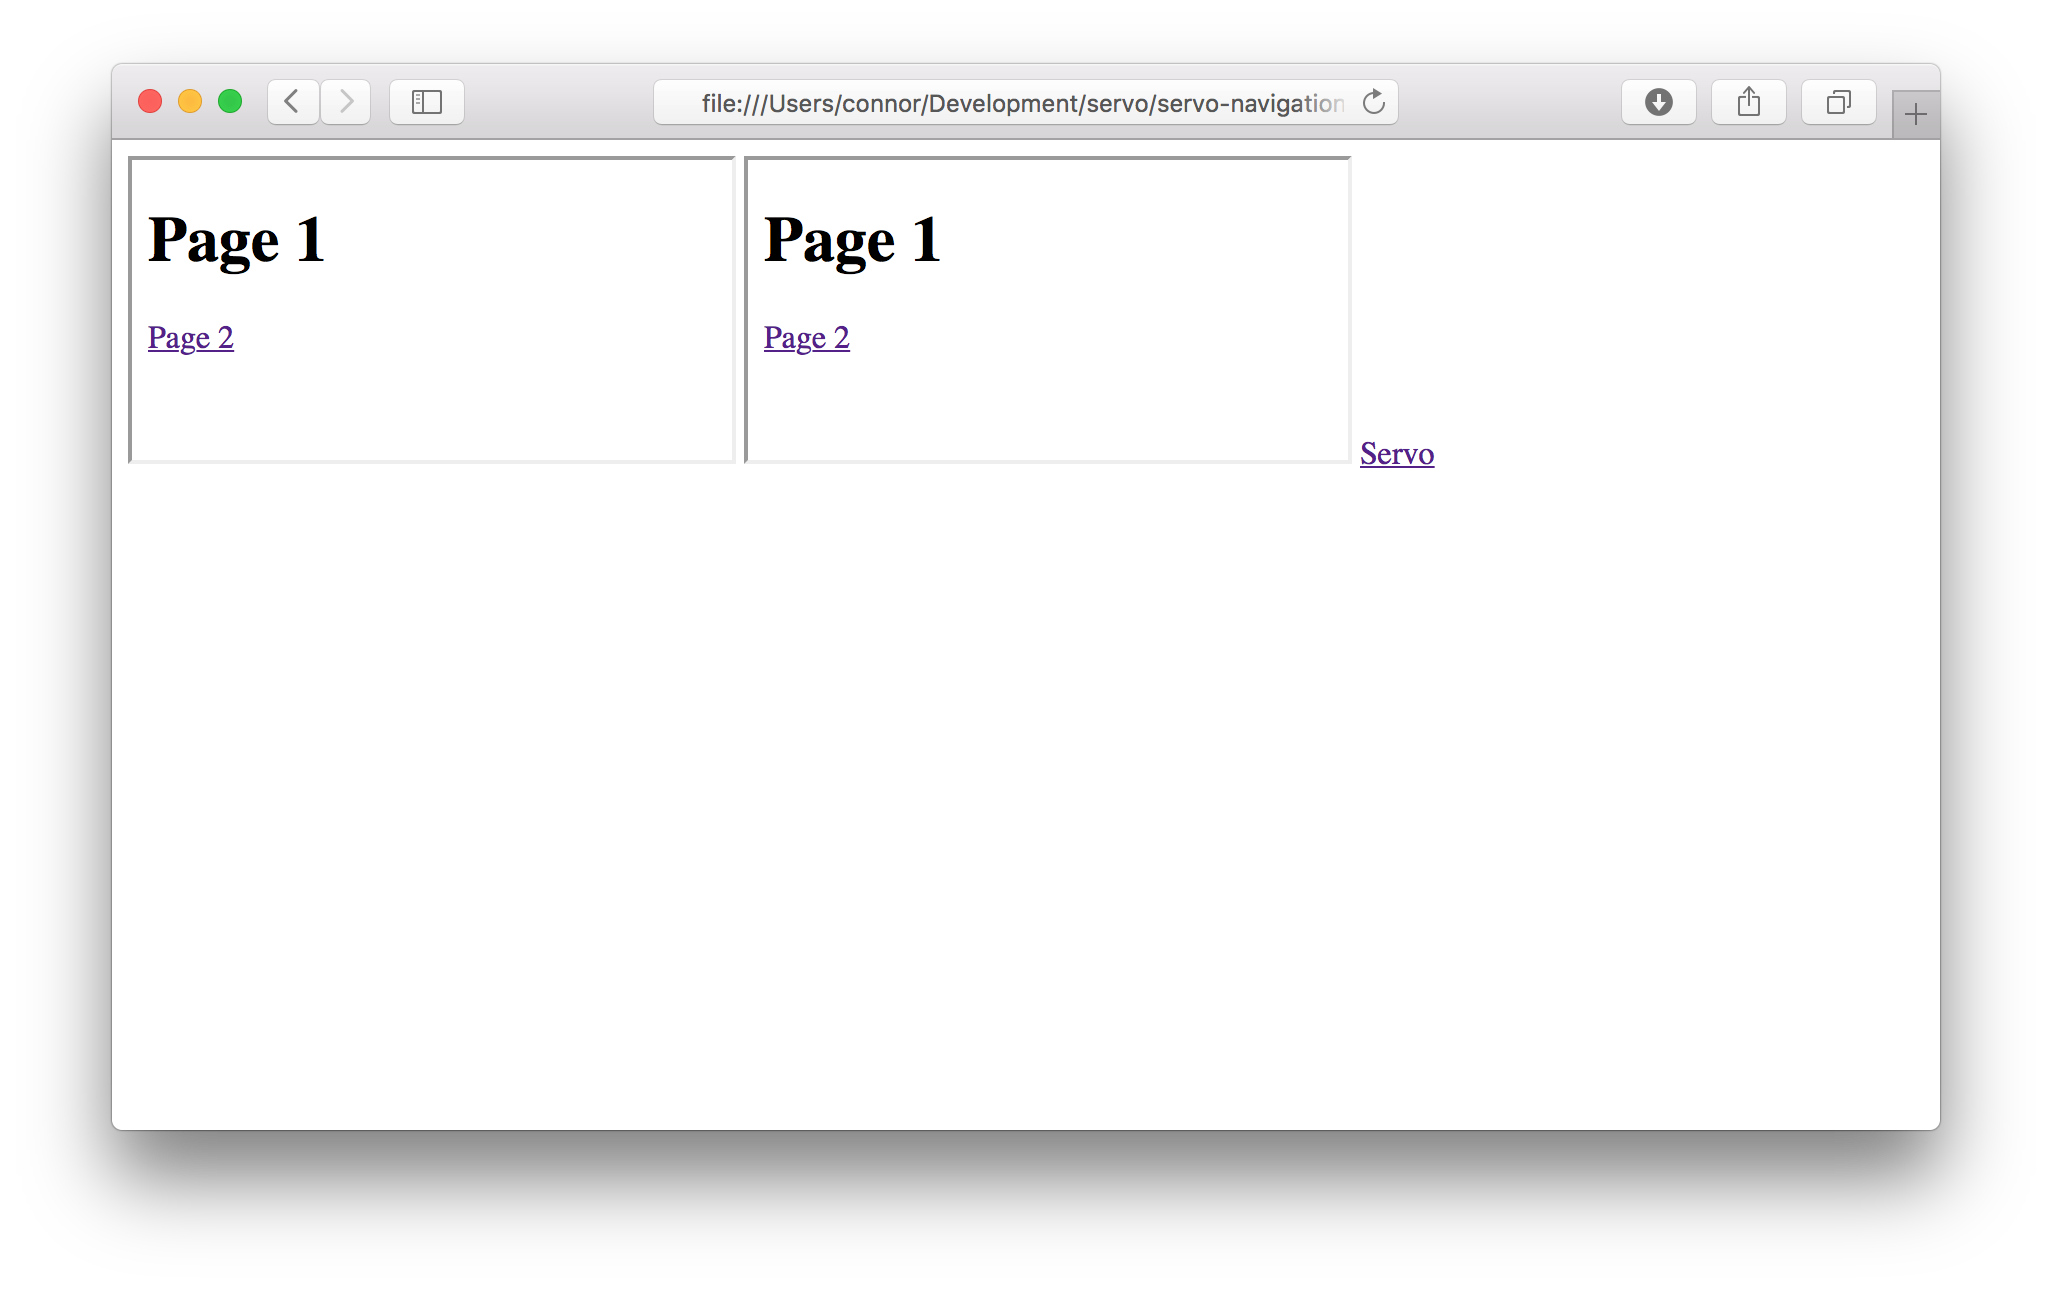
\includegraphics[width=.5\linewidth]{images/experiments/forwardback4/safari/1.png}%
    }~\raisebox{-.5\height}{
      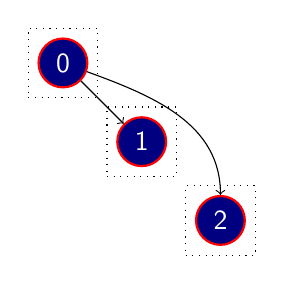
\begin{tikzpicture}
        \node[doc,active,fully](0) at (0,0){0};
        \node[doc,active,fully](1) at (1,-1){1};
        \node[doc,jshactive,fully](2) at (2,-2){2};
        \node[draw,dotted,fit=(0)]{};
        \node[draw,dotted,fit=(1)]{};
        \node[draw,dotted,fit=(2)]{};
        \draw[->](0)--(1);
        \draw[->](0)to[out=-20,in=90](2);
      \end{tikzpicture}
    }
    \caption{Initial State}
  \end{figure}

  Navigate document $1$ to Page 2:
  \begin{figure}[H]
    \raisebox{-.5\height}{
      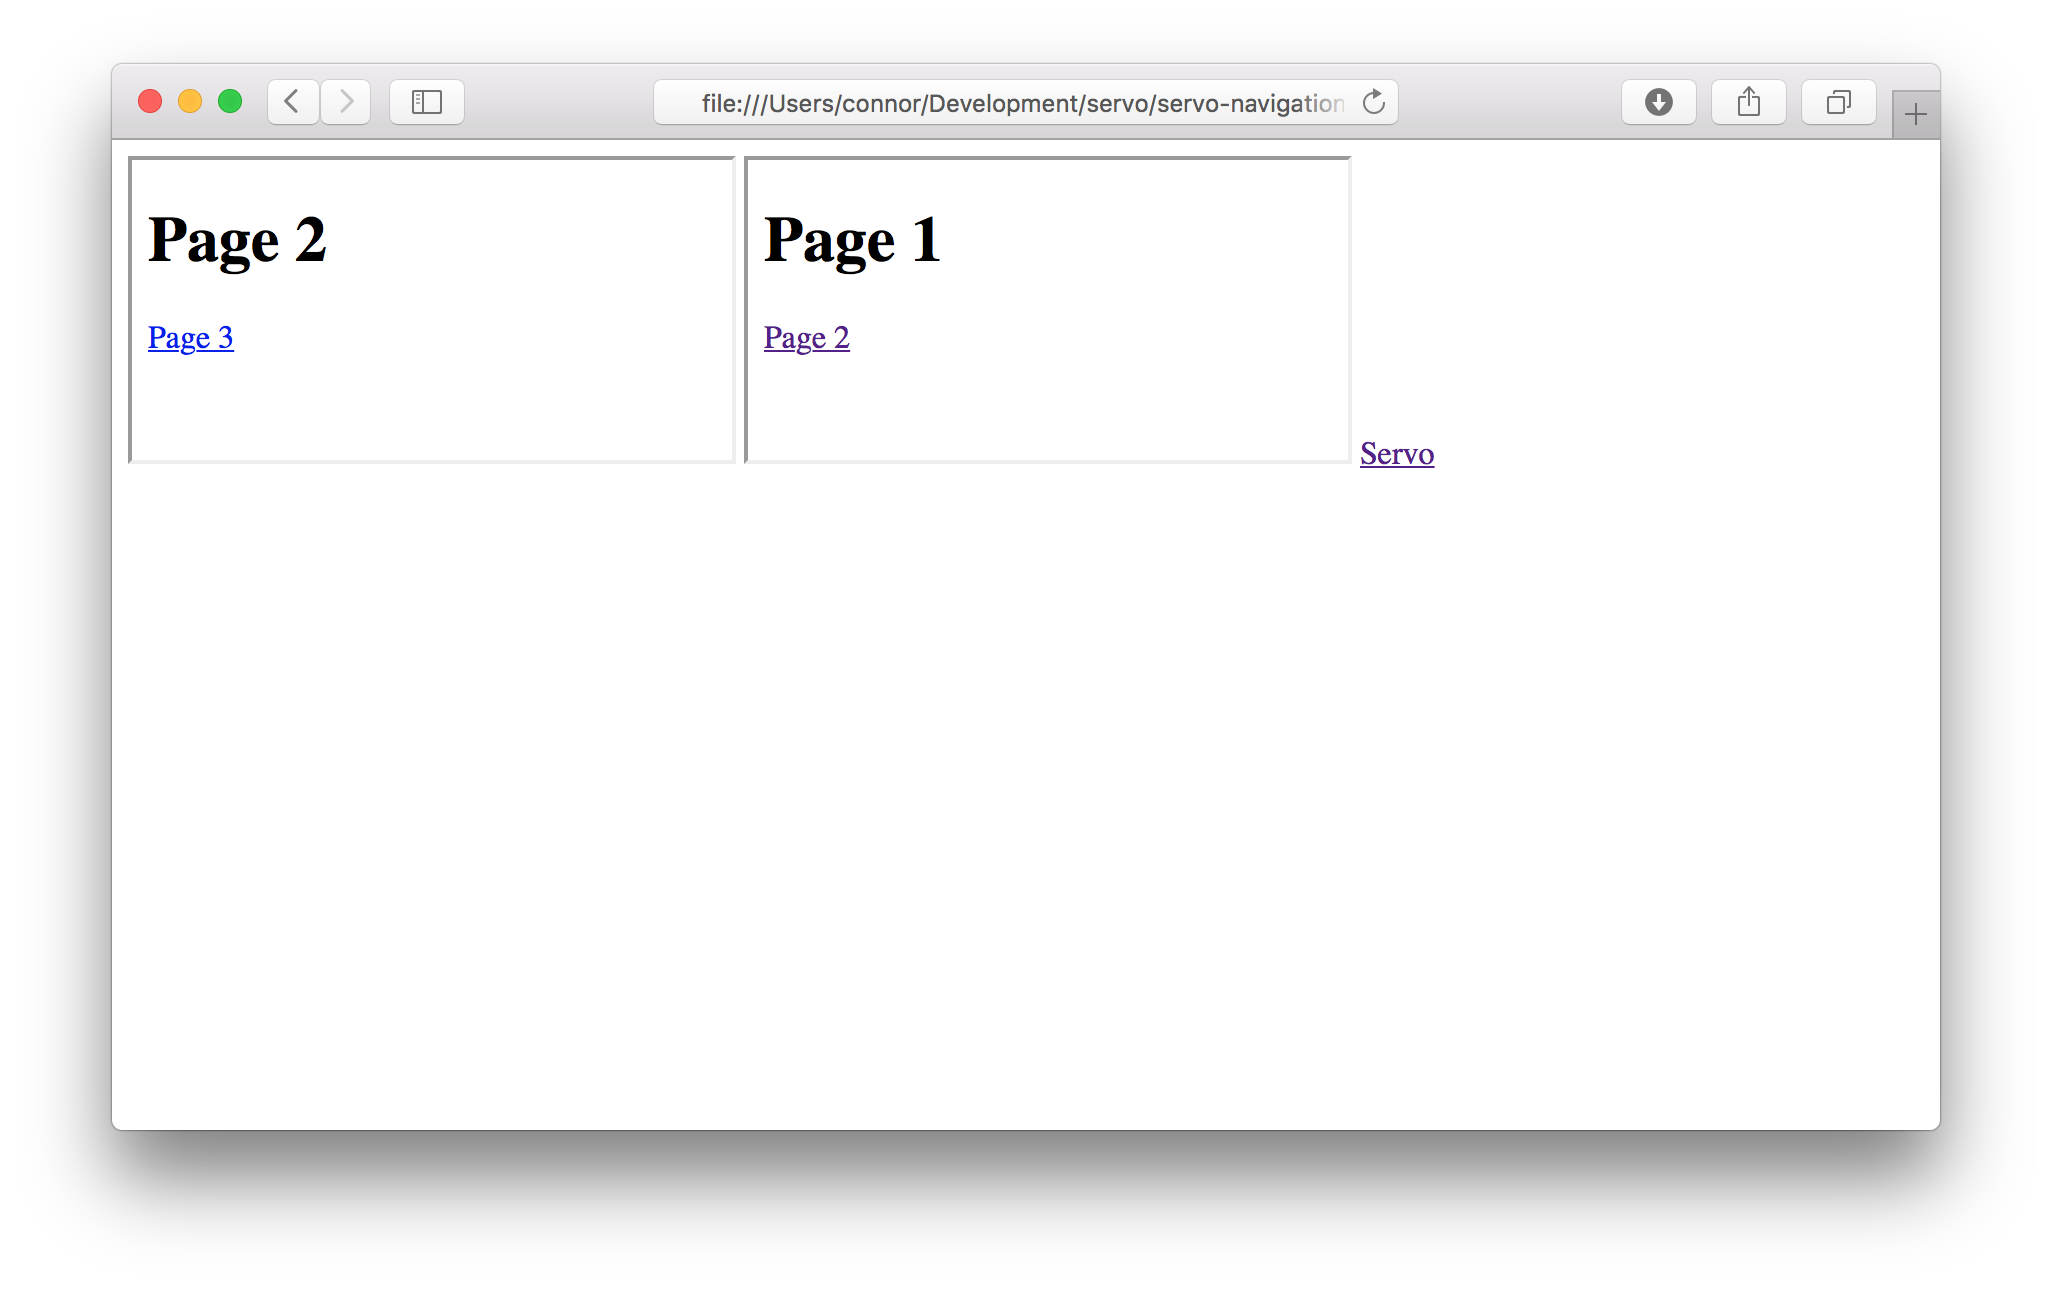
\includegraphics[width=.5\linewidth]{images/experiments/forwardback4/safari/2.png}
    }~\raisebox{-.5\height}{
      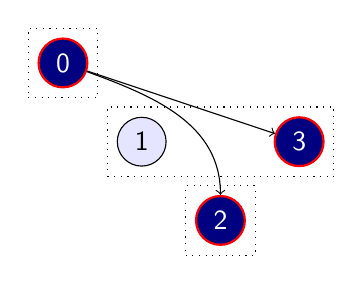
\begin{tikzpicture}
        \node[doc,active,fully](0) at (0,0){0};
        \node[doc](1) at (1,-1){1};
        \node[doc,active,fully](2) at (2,-2){2};
        \node[doc,jshactive,fully](3) at (3,-1){3};
        \node[draw,dotted,fit=(0)]{};
        \node[draw,dotted,fit=(1)(3)]{};
        \node[draw,dotted,fit=(2)]{};
        \draw[->](0)--(3);
        \draw[->](0)to[out=-20,in=90](2);
      \end{tikzpicture}
    }
    \caption{Navigate document $1$ to Page 2.}
  \end{figure}

  Navigate document $3$ to Page 3:
  \begin{figure}[H]
    \raisebox{-.5\height}{
      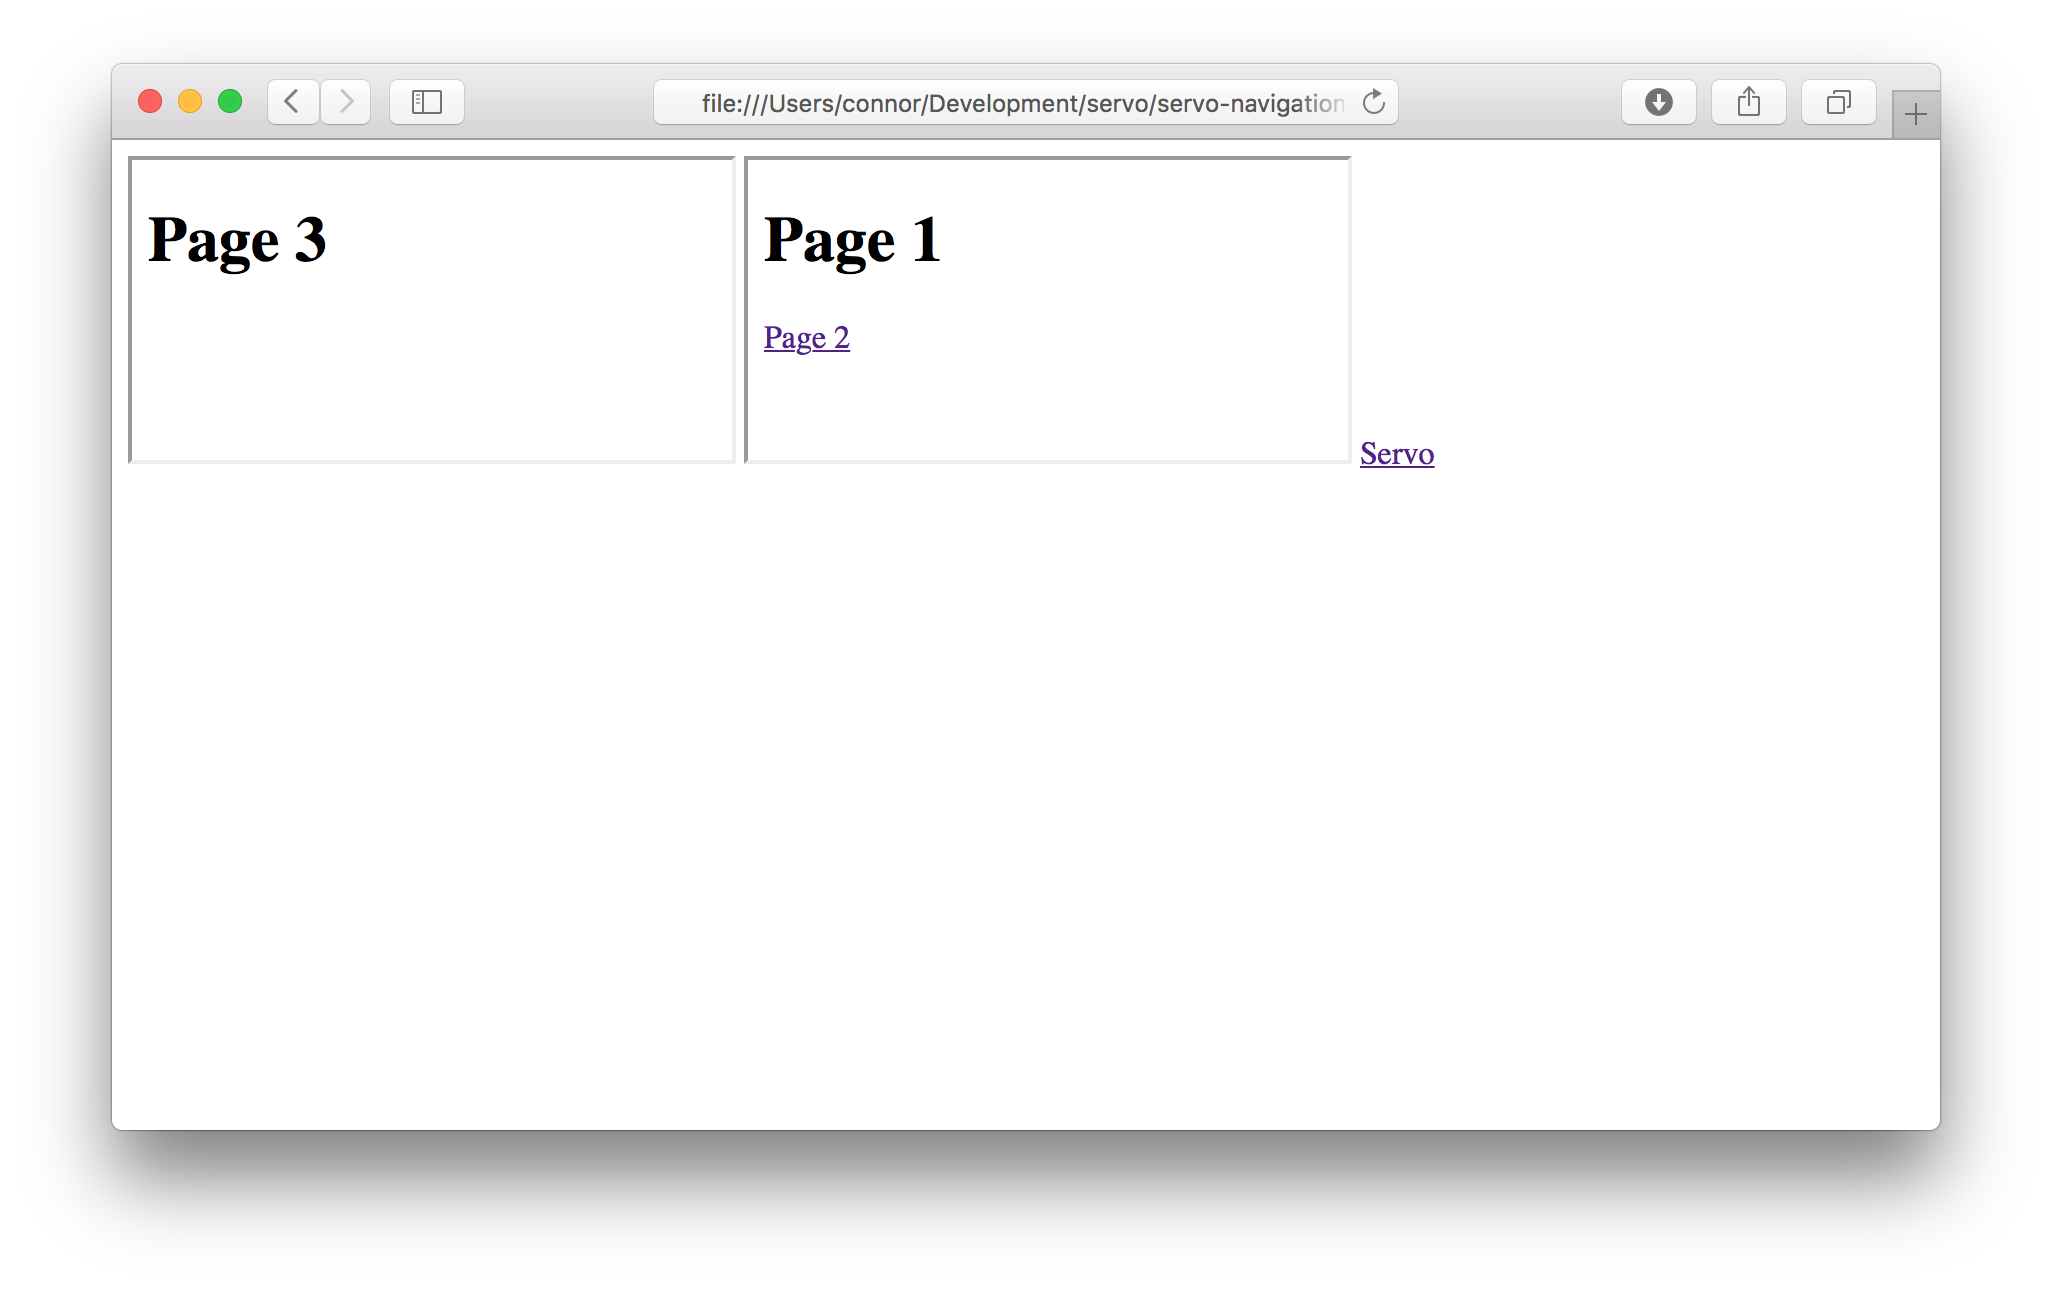
\includegraphics[width=.5\linewidth]{images/experiments/forwardback4/safari/3.png}
    }~\raisebox{-.5\height}{
      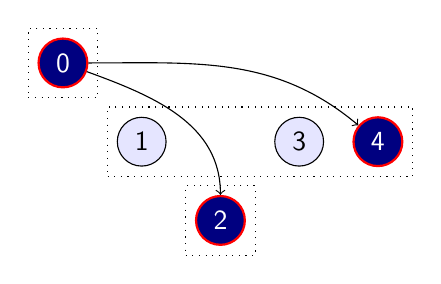
\begin{tikzpicture}
        \node[doc,active,fully](0) at (0,0){0};
        \node[doc](1) at (1,-1){1};
        \node[doc,active,fully](2) at (2,-2){2};
        \node[doc](3) at (3,-1){3};
        \node[doc,jshactive,fully](4) at (4,-1){4};
        \node[draw,dotted,fit=(0)]{};
        \node[draw,dotted,fit=(1)(4)]{};
        \node[draw,dotted,fit=(2)]{};
        \draw[->](0)to[out=0,in=140](4);
        \draw[->](0)to[out=-20,in=90](2);
      \end{tikzpicture}
    }
    \caption{Navigate document $3$ to Page 3.}
  \end{figure}

  Navigate document $2$ to Page 2:
  \begin{figure}[H]
    \raisebox{-.5\height}{
      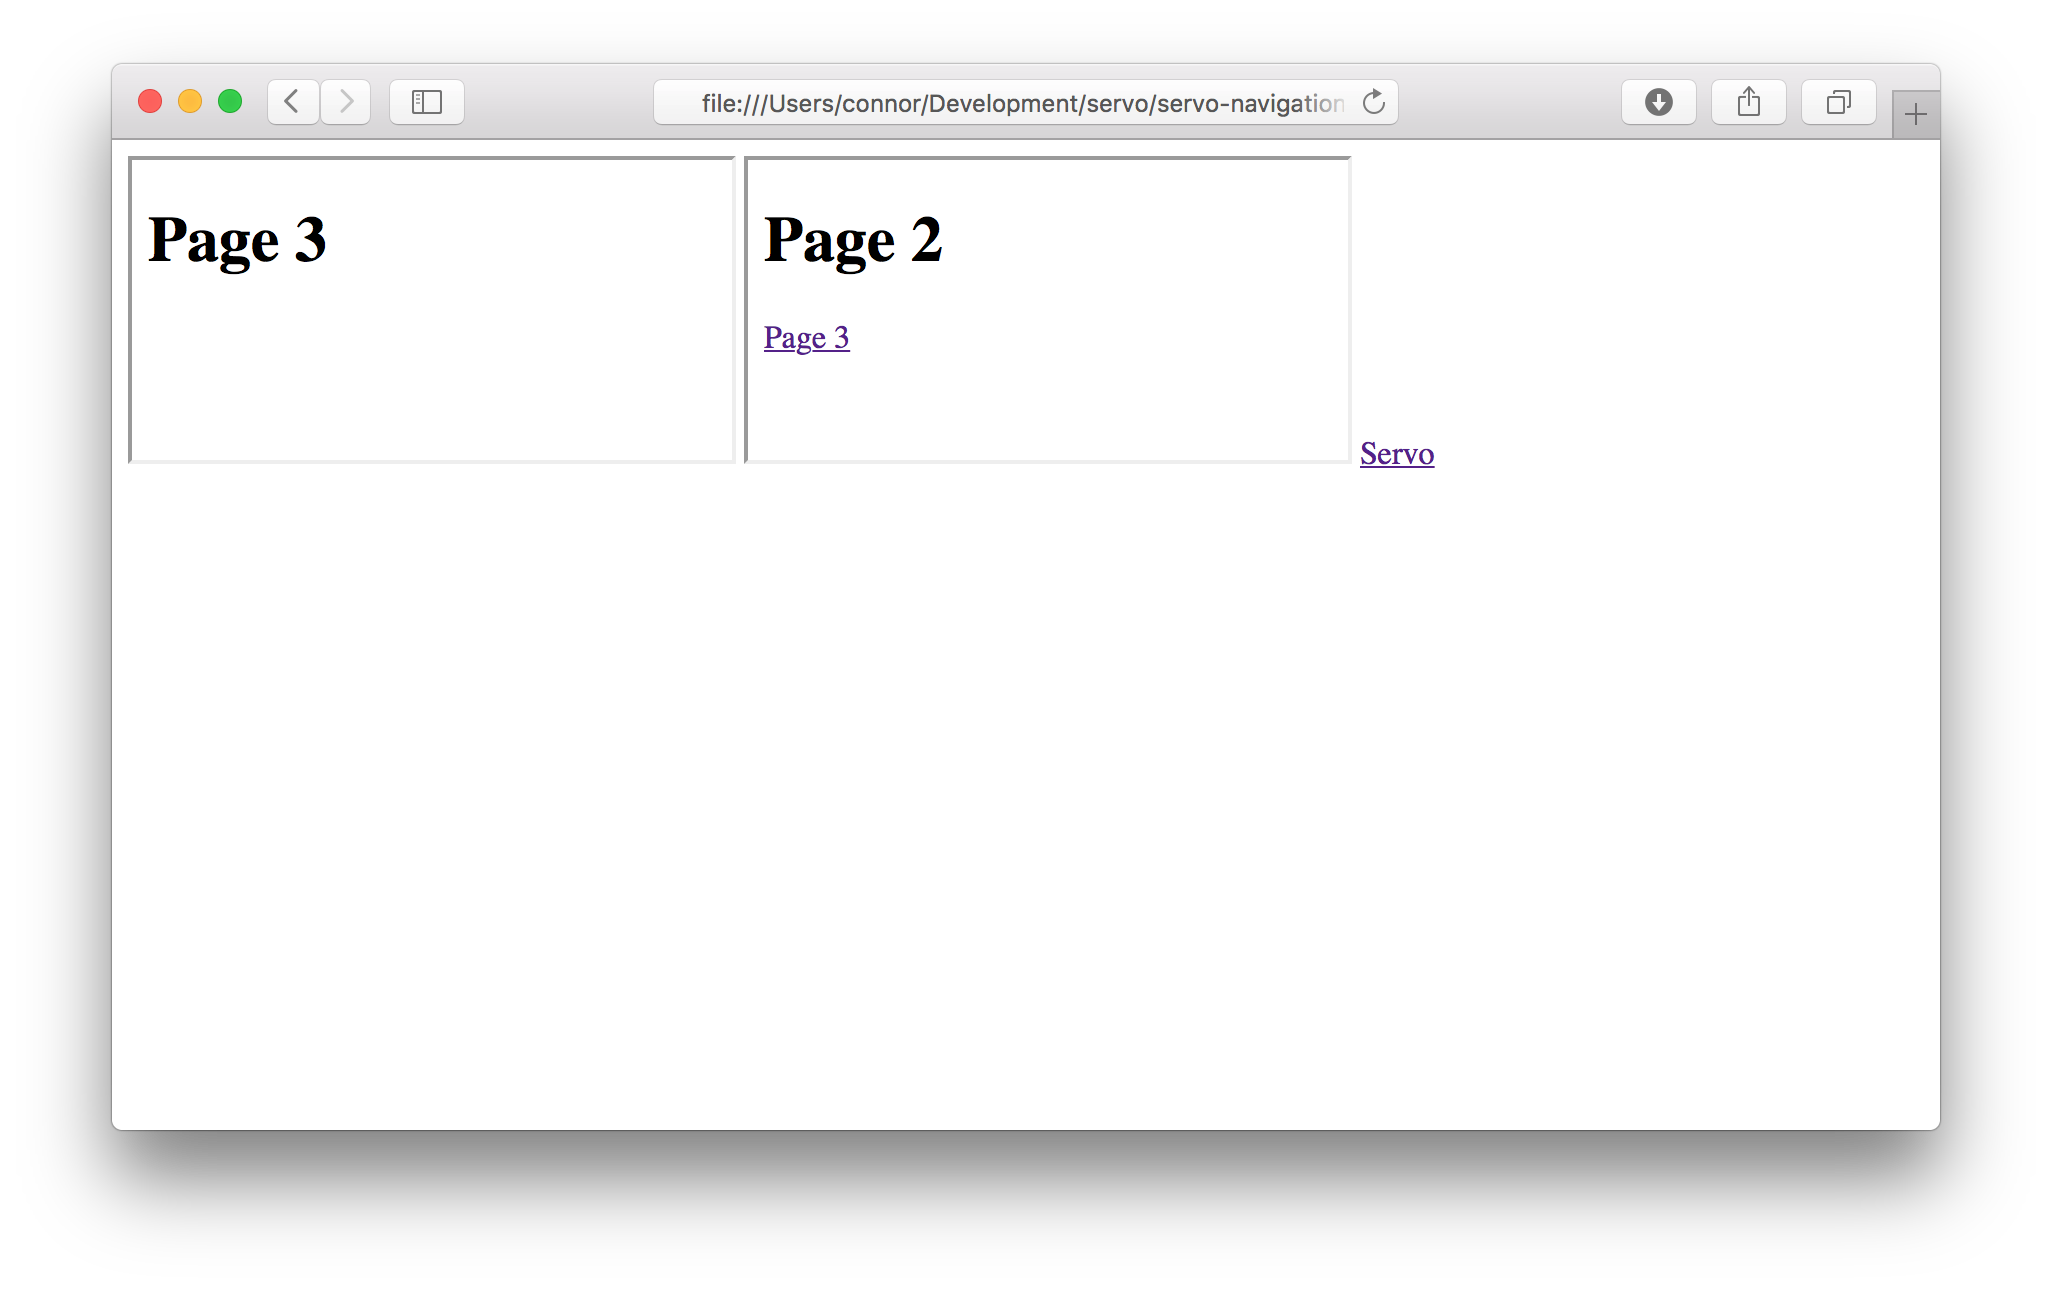
\includegraphics[width=.5\linewidth]{images/experiments/forwardback4/safari/4.png}
    }~\raisebox{-.5\height}{
      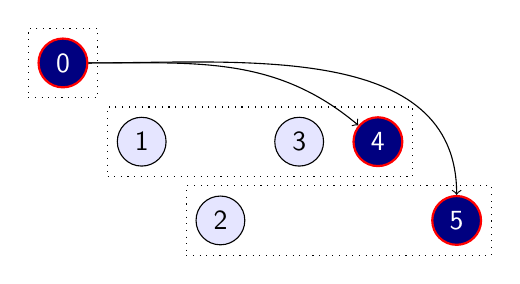
\begin{tikzpicture}
        \node[doc,active,fully](0) at (0,0){0};
        \node[doc](1) at (1,-1){1};
        \node[doc](2) at (2,-2){2};
        \node[doc](3) at (3,-1){3};
        \node[doc,active,fully](4) at (4,-1){4};
        \node[doc,jshactive,fully](5) at (5,-2){5};
        \node[draw,dotted,fit=(0)]{};
        \node[draw,dotted,fit=(1)(4)]{};
        \node[draw,dotted,fit=(2)(5)]{};
        \draw[->](0)to[out=0,in=140](4);
        \draw[->](0)to[out=0,in=90](5);
      \end{tikzpicture}
    }
    \caption{Navigate document $2$ to Page 2.}
  \end{figure}

  Navigate document $5$ to Page 3:
  \begin{figure}[H]
    \raisebox{-.5\height}{
      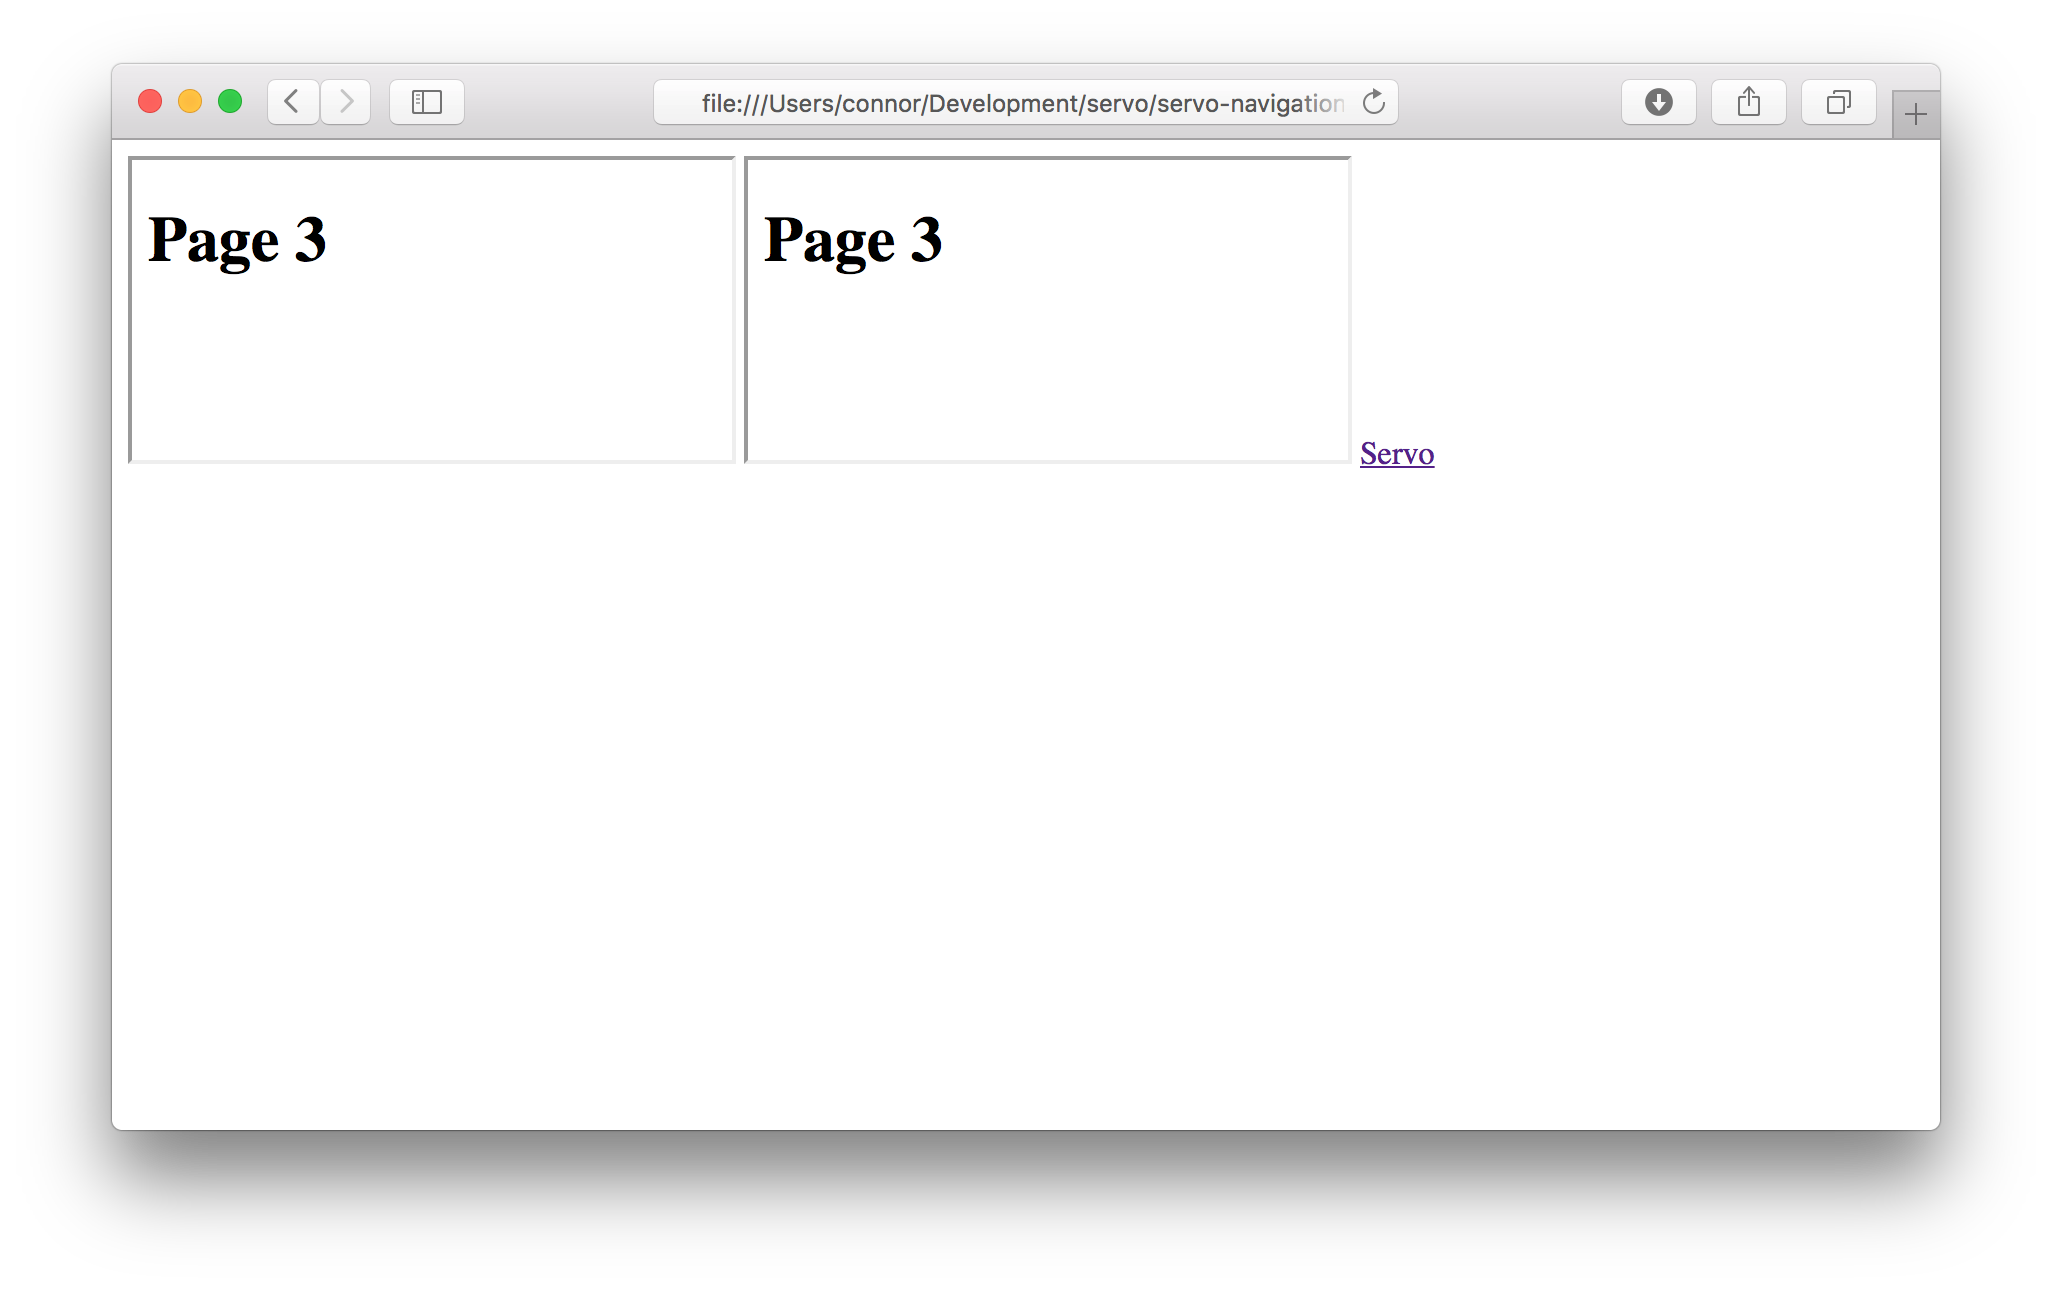
\includegraphics[width=.5\linewidth]{images/experiments/forwardback4/safari/5.png}
    }~\raisebox{-.5\height}{
      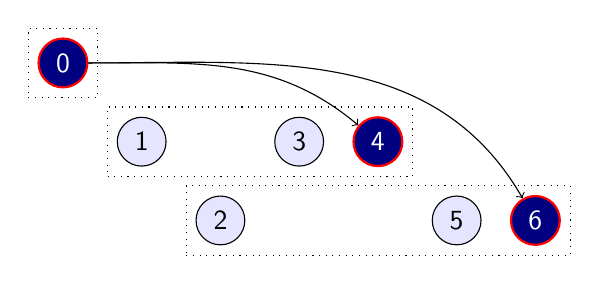
\begin{tikzpicture}
        \node[doc,active,fully](0) at (0,0){0};
        \node[doc](1) at (1,-1){1};
        \node[doc](2) at (2,-2){2};
        \node[doc](3) at (3,-1){3};
        \node[doc,active,fully](4) at (4,-1){4};
        \node[doc](5) at (5,-2){5};
        \node[doc,jshactive,fully](6) at (6,-2){6};
        \node[draw,dotted,fit=(0)]{};
        \node[draw,dotted,fit=(1)(4)]{};
        \node[draw,dotted,fit=(2)(6)]{};
        \draw[->](0)to[out=0,in=140](4);
        \draw[->](0)to[out=0,in=120](6);
      \end{tikzpicture}
    }
    \caption{Navigate document $5$ to Page 3.}
  \end{figure}

  \emph{$\aNH$ traverses the history by $-4$ to $\aNH'$}:
  \begin{figure}[H]
    \raisebox{-.5\height}{
      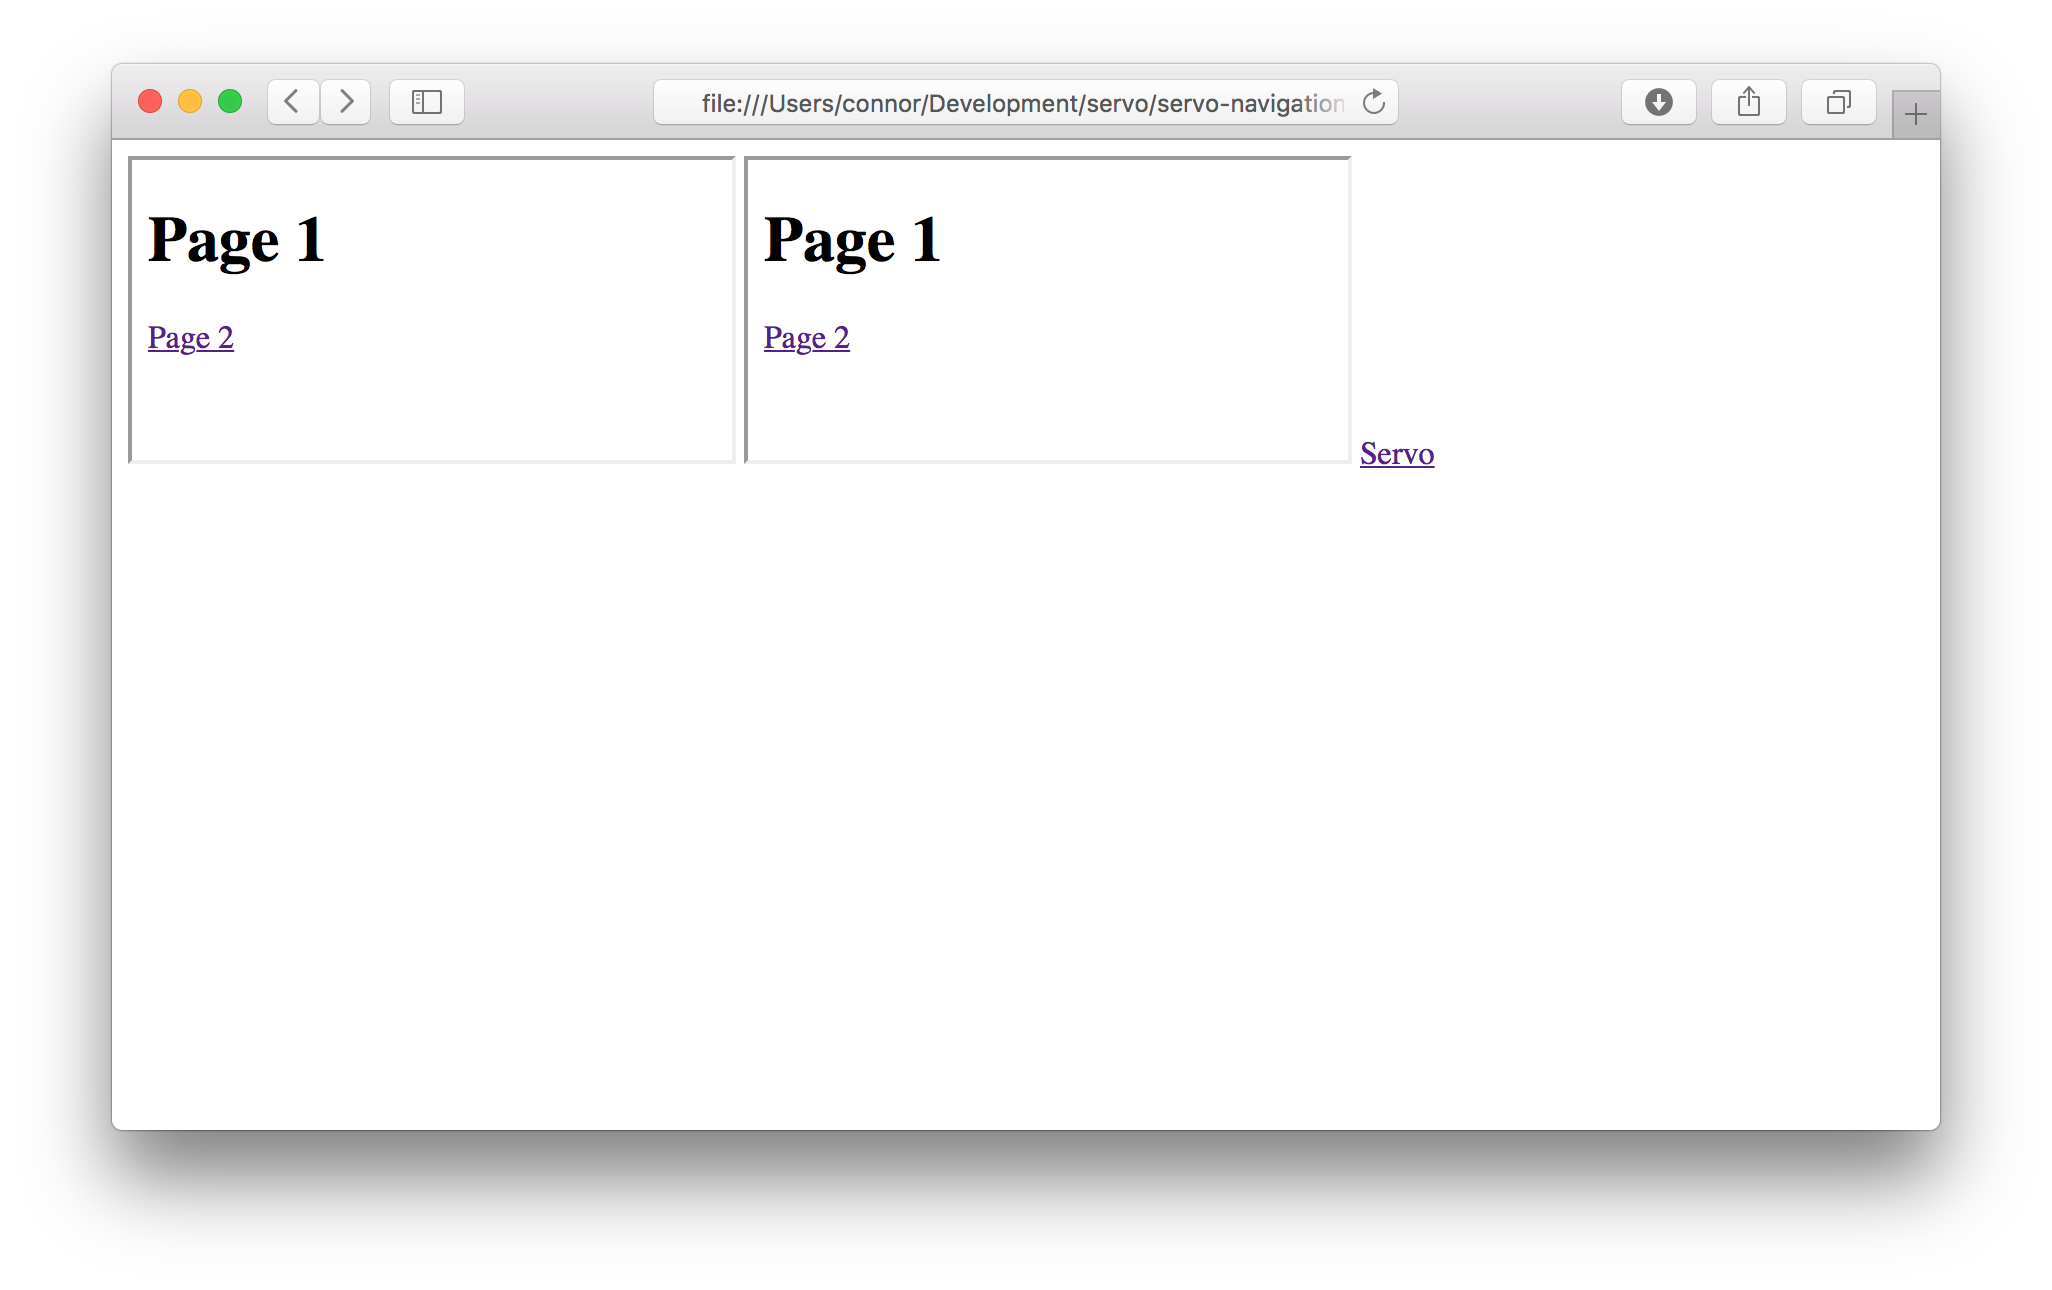
\includegraphics[width=.5\linewidth]{images/experiments/forwardback4/safari/6.png}
    }~\raisebox{-.5\height}{
      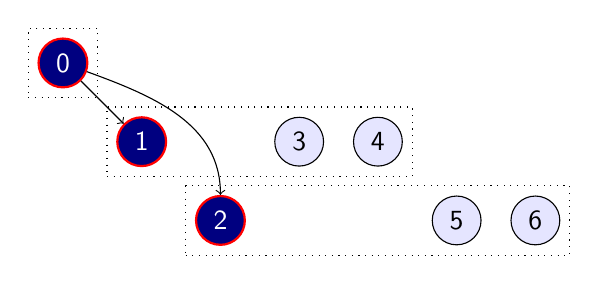
\begin{tikzpicture}
        \node[doc,active,fully](0) at (0,0){0};
        \node[doc,active,fully](1) at (1,-1){1};
        \node[doc,jshactive,fully](2) at (2,-2){2};
        \node[doc](3) at (3,-1){3};
        \node[doc](4) at (4,-1){4};
        \node[doc](5) at (5,-2){5};
        \node[doc](6) at (6,-2){6};
        \node[draw,dotted,fit=(0)]{};
        \node[draw,dotted,fit=(1)(4)]{};
        \node[draw,dotted,fit=(2)(6)]{};
        \draw[->](0)--(1);
        \draw[->](0)to[out=-20,in=90](2);
      \end{tikzpicture}
    }
    \caption{Traversal by $-4$.}
  \end{figure}

  \emph{$\aNH'$ traverses the history by $4$ to $\aNH''$}:
  \begin{figure}[H]
    \raisebox{-.5\height}{
      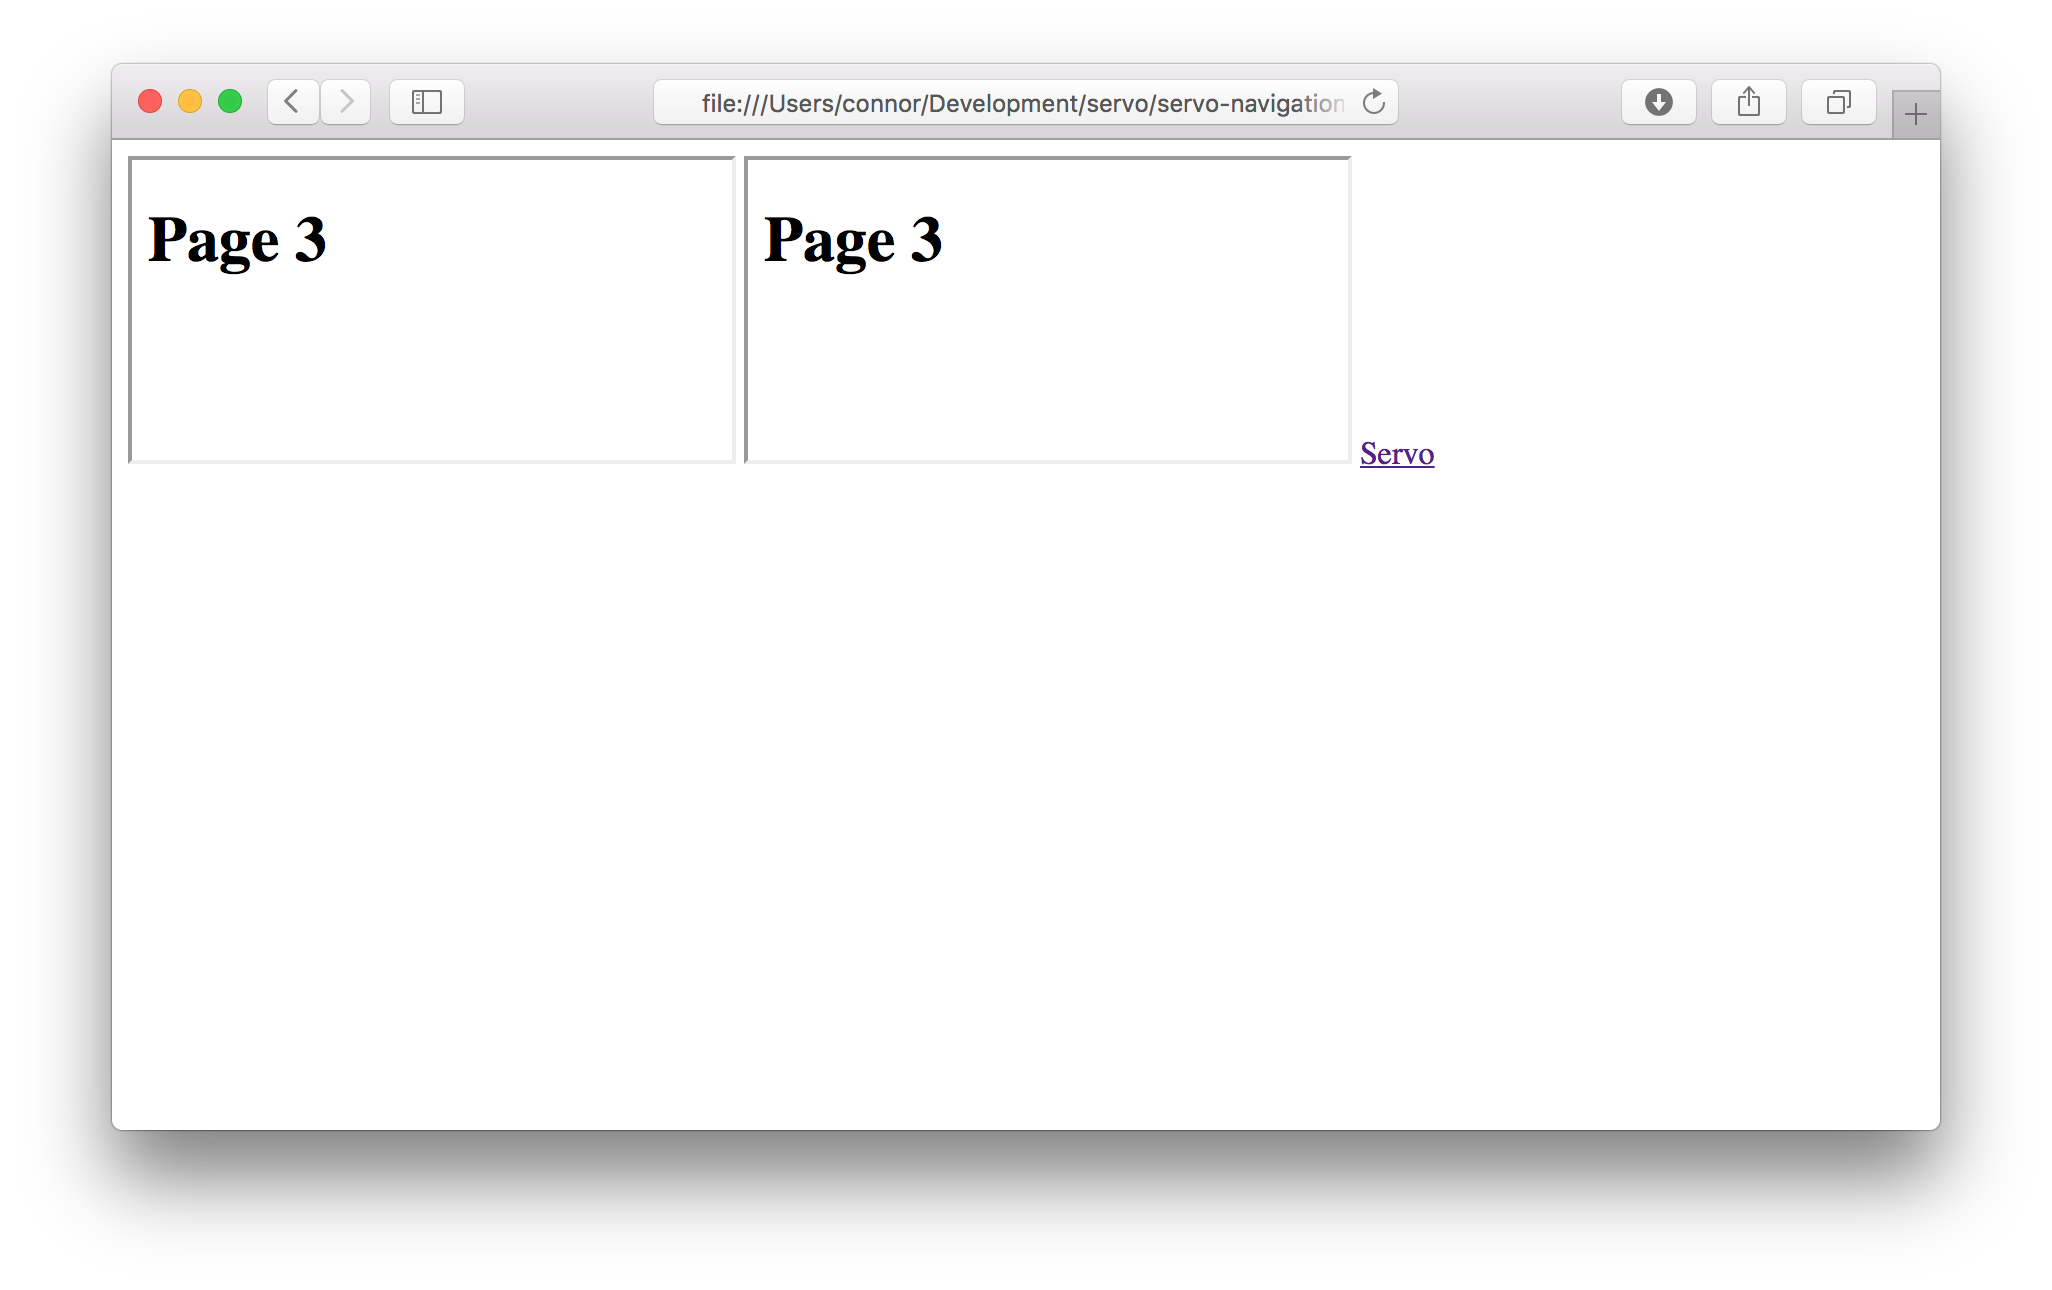
\includegraphics[width=.5\linewidth]{images/experiments/forwardback4/safari/7.png}
    }~\raisebox{-.5\height}{
      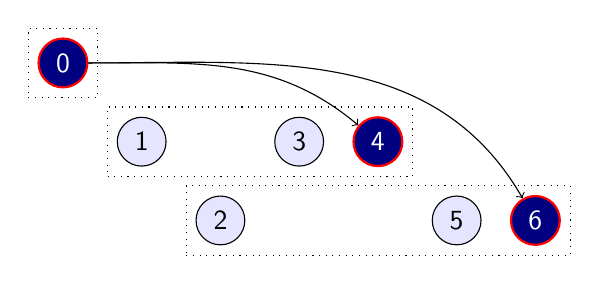
\begin{tikzpicture}
        \node[doc,active,fully](0) at (0,0){0};
        \node[doc](1) at (1,-1){1};
        \node[doc](2) at (2,-2){2};
        \node[doc](3) at (3,-1){3};
        \node[doc,active,fully](4) at (4,-1){4};
        \node[doc](5) at (5,-2){5};
        \node[doc,jshactive,fully](6) at (6,-2){6};
        \node[draw,dotted,fit=(0)]{};
        \node[draw,dotted,fit=(1)(4)]{};
        \node[draw,dotted,fit=(2)(6)]{};
        \draw[->](0)to[out=0,in=140](4);
        \draw[->](0)to[out=0,in=120](6);
      \end{tikzpicture}
    }
    \caption{Traversal by $4$.}
  \end{figure}

  These results in Safari satisfy Goal~\ref{goal:homomorphism}.

  Chrome:
  \begin{figure}[H]
    \raisebox{-.5\height}{
      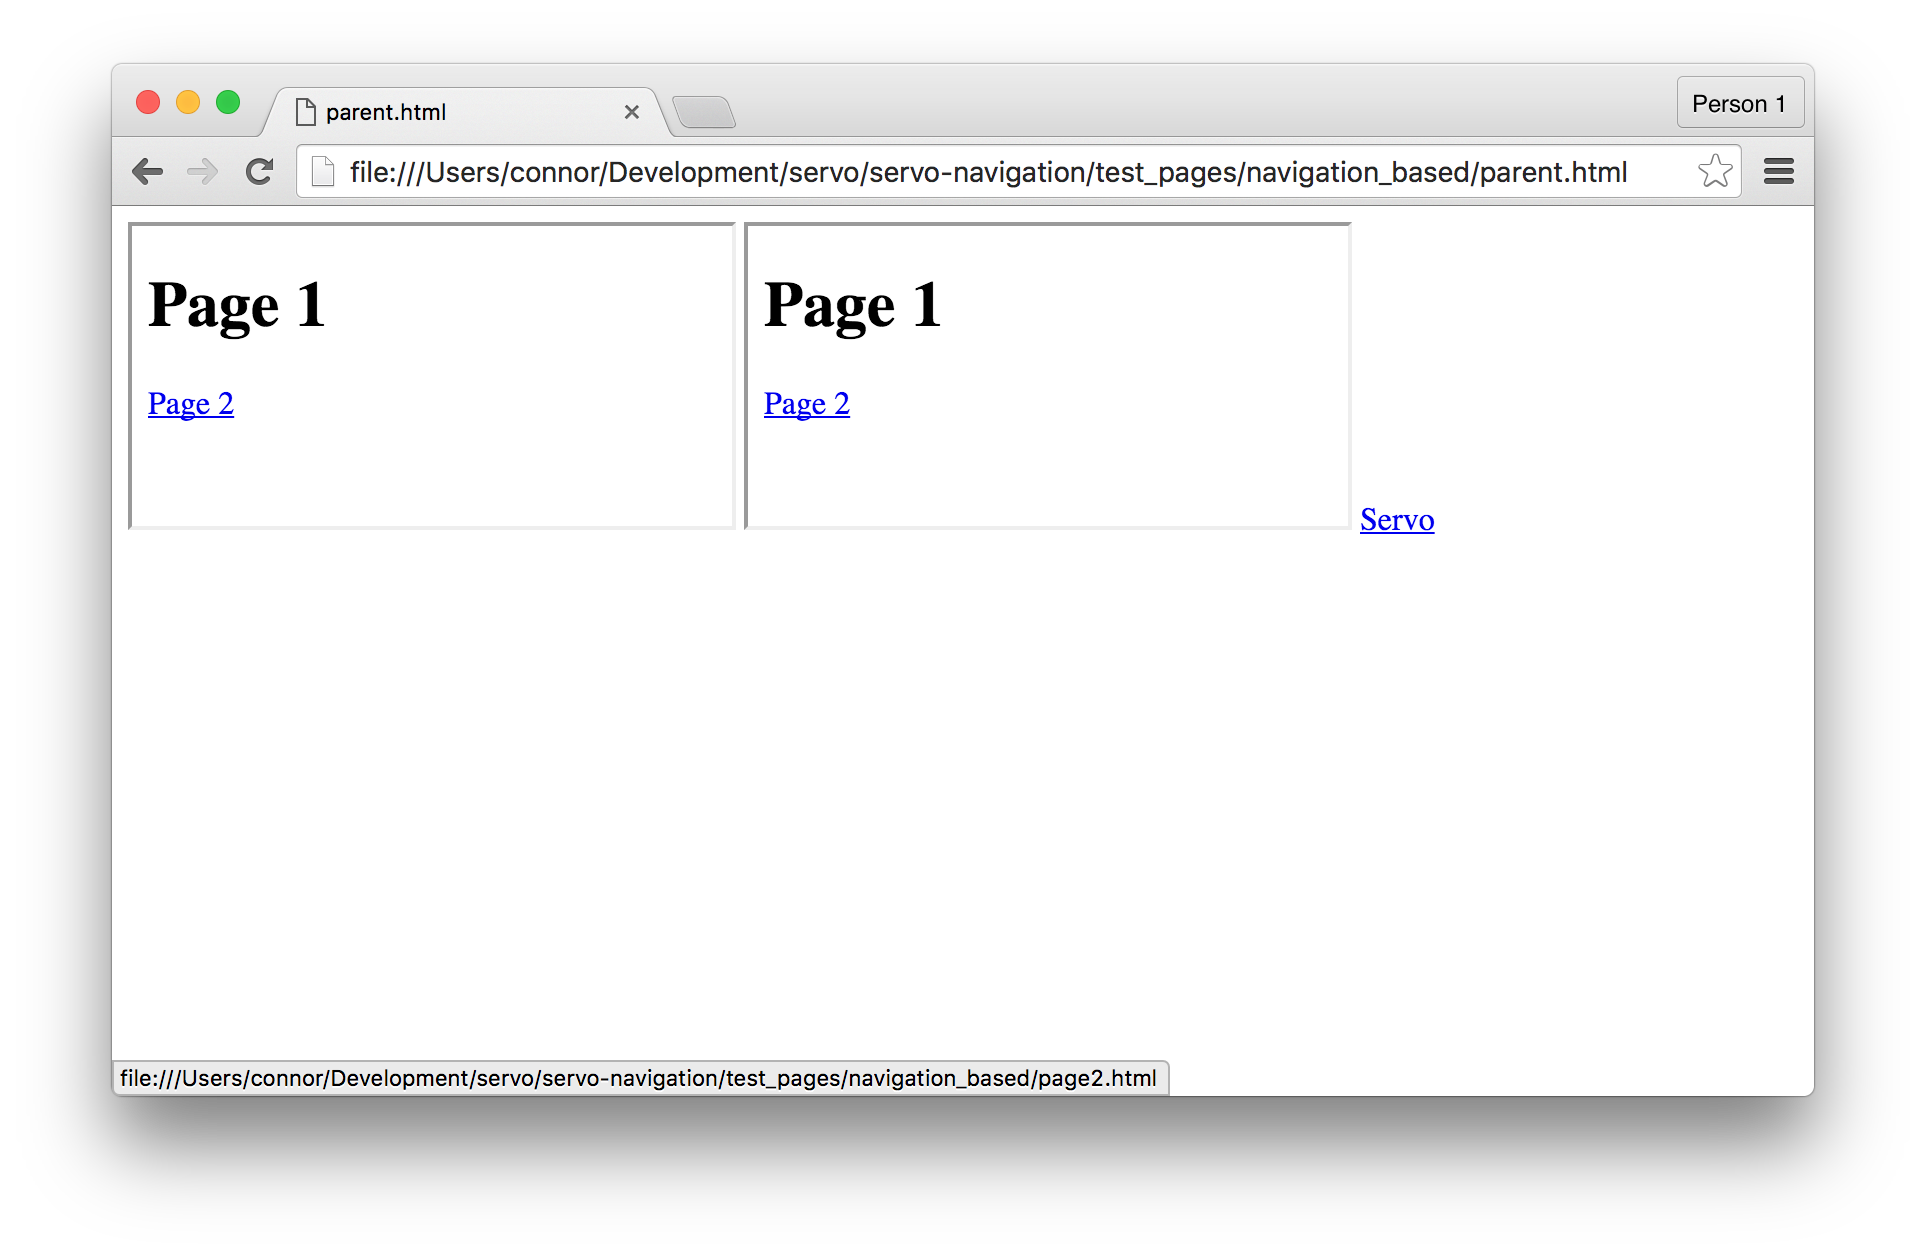
\includegraphics[width=.5\linewidth]{images/experiments/forwardback4/chrome/1.png}%
    }~\raisebox{-.5\height}{
      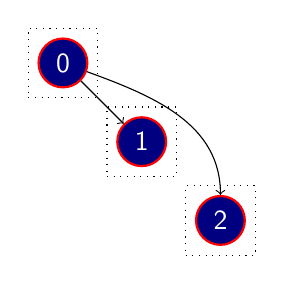
\begin{tikzpicture}
        \node[doc,active,fully](0) at (0,0){0};
        \node[doc,active,fully](1) at (1,-1){1};
        \node[doc,jshactive,fully](2) at (2,-2){2};
        \node[draw,dotted,fit=(0)]{};
        \node[draw,dotted,fit=(1)]{};
        \node[draw,dotted,fit=(2)]{};
        \draw[->](0)--(1);
        \draw[->](0)to[out=-20,in=90](2);
      \end{tikzpicture}
    }
    \caption{Initial State}
  \end{figure}

  Navigate document $1$ to Page 2:
  \begin{figure}[H]
    \raisebox{-.5\height}{
      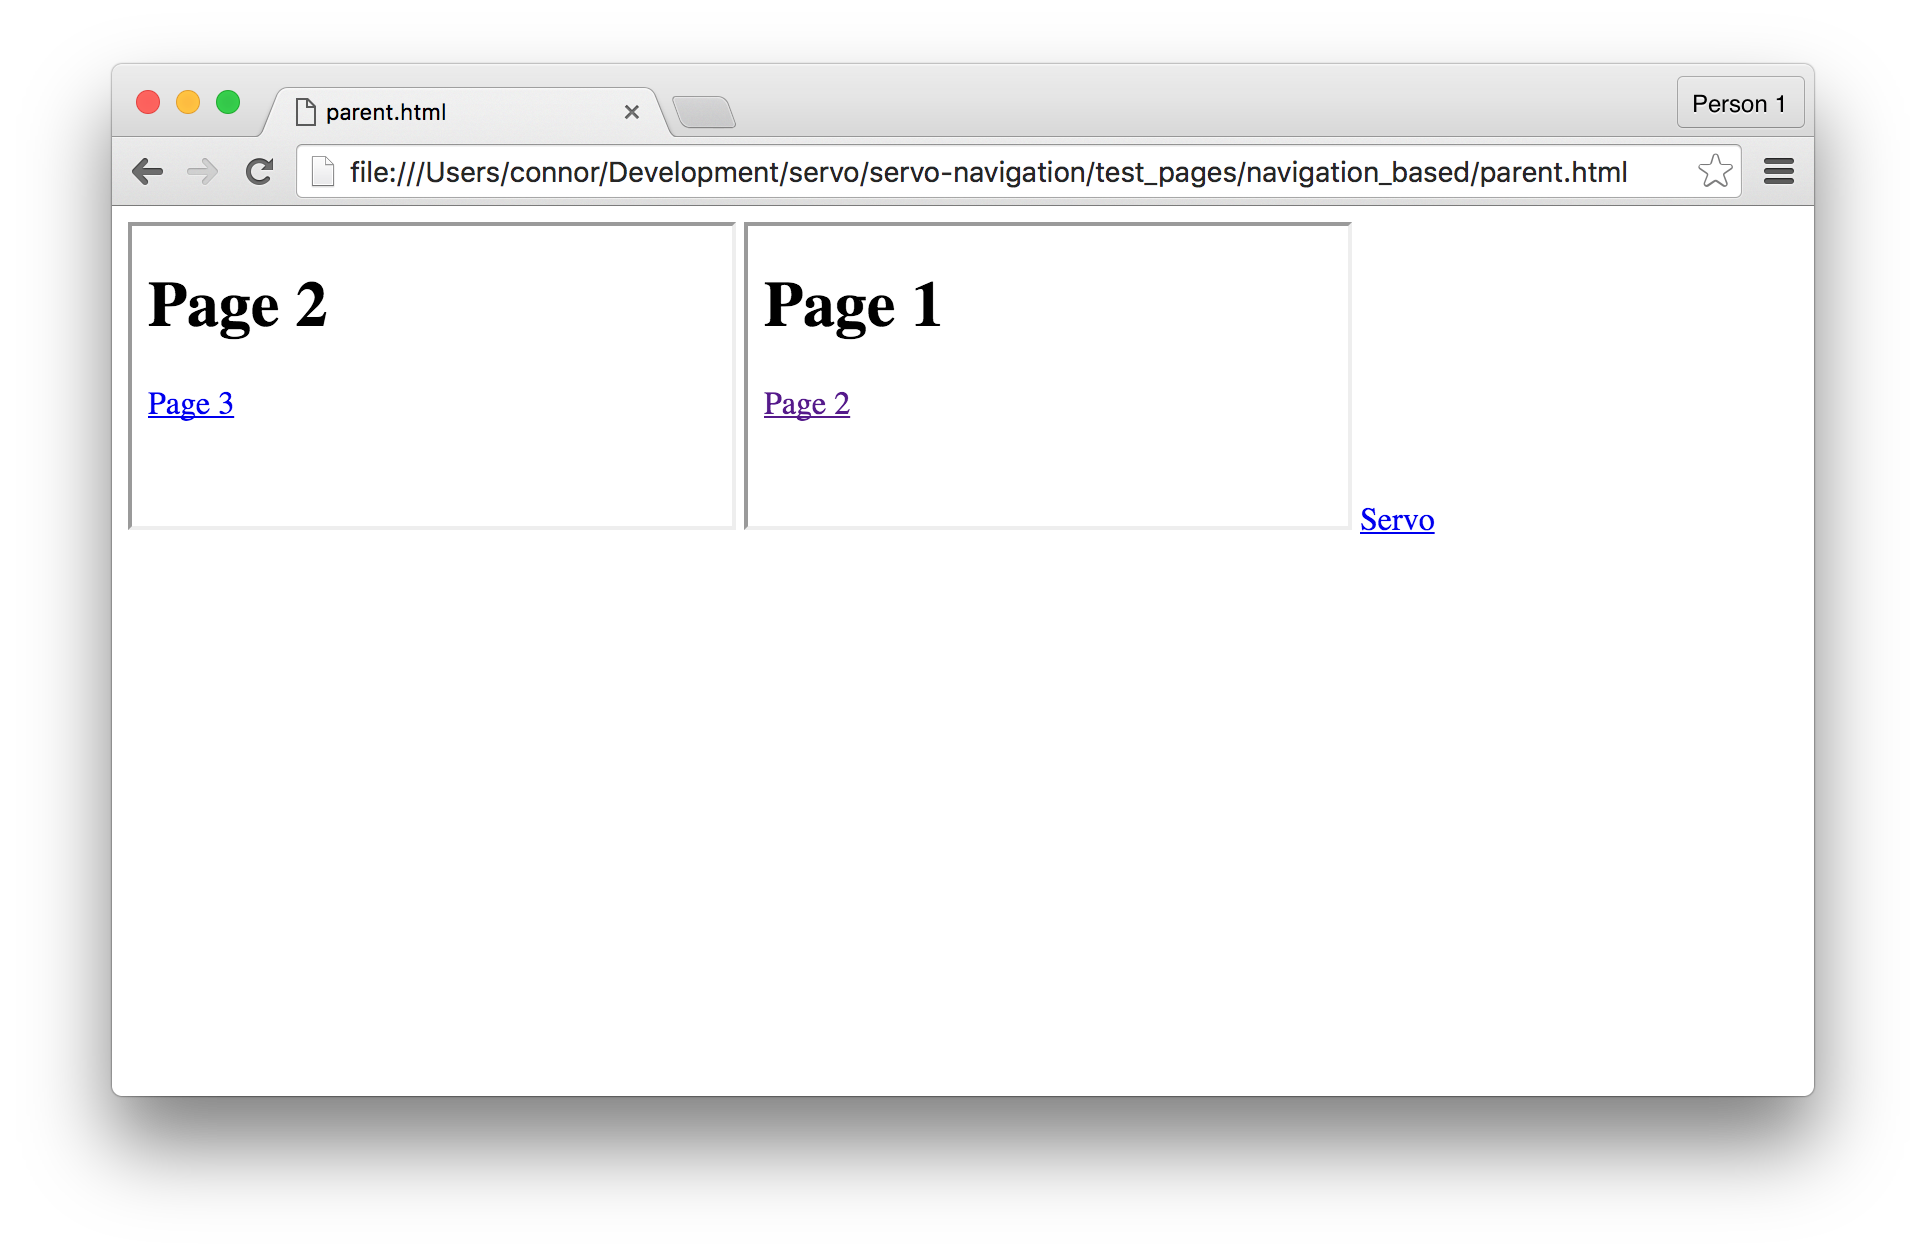
\includegraphics[width=.5\linewidth]{images/experiments/forwardback4/chrome/2.png}
    }~\raisebox{-.5\height}{
      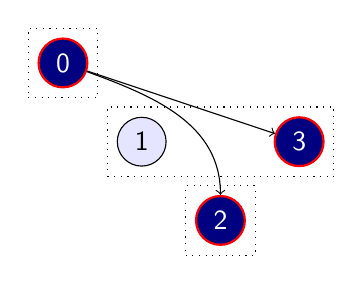
\begin{tikzpicture}
        \node[doc,active,fully](0) at (0,0){0};
        \node[doc](1) at (1,-1){1};
        \node[doc,active,fully](2) at (2,-2){2};
        \node[doc,jshactive,fully](3) at (3,-1){3};
        \node[draw,dotted,fit=(0)]{};
        \node[draw,dotted,fit=(1)(3)]{};
        \node[draw,dotted,fit=(2)]{};
        \draw[->](0)--(3);
        \draw[->](0)to[out=-20,in=90](2);
      \end{tikzpicture}
    }
    \caption{Navigate document $1$ to Page 2.}
  \end{figure}

  Navigate document $3$ to Page 3:
  \begin{figure}[H]
    \raisebox{-.5\height}{
      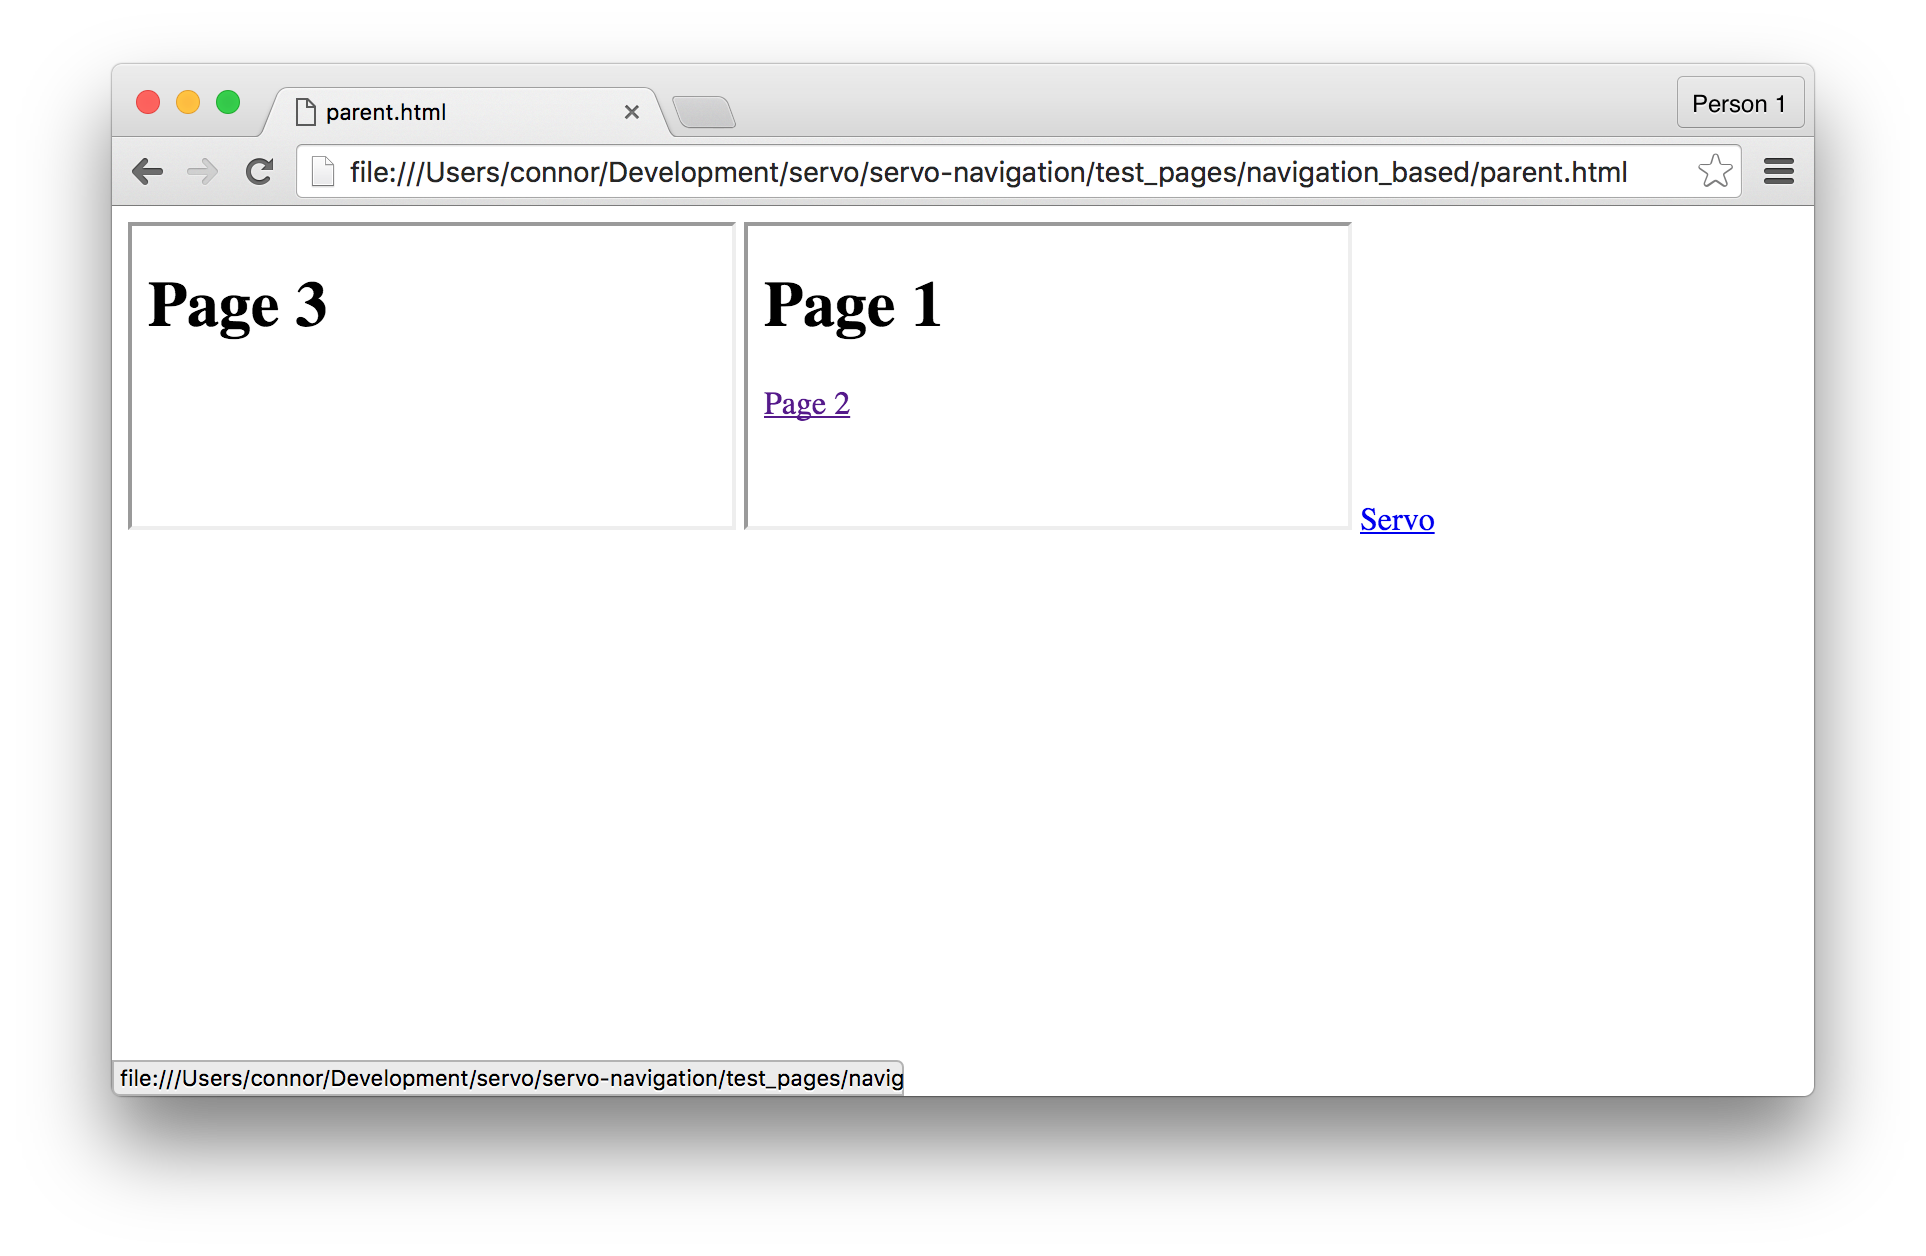
\includegraphics[width=.5\linewidth]{images/experiments/forwardback4/chrome/3.png}
    }~\raisebox{-.5\height}{
      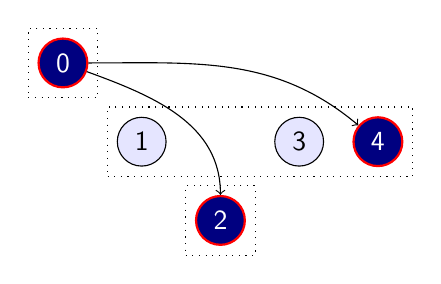
\begin{tikzpicture}
        \node[doc,active,fully](0) at (0,0){0};
        \node[doc](1) at (1,-1){1};
        \node[doc,active,fully](2) at (2,-2){2};
        \node[doc](3) at (3,-1){3};
        \node[doc,jshactive,fully](4) at (4,-1){4};
        \node[draw,dotted,fit=(0)]{};
        \node[draw,dotted,fit=(1)(4)]{};
        \node[draw,dotted,fit=(2)]{};
        \draw[->](0)to[out=0,in=140](4);
        \draw[->](0)to[out=-20,in=90](2);
      \end{tikzpicture}
    }
    \caption{Navigate document $3$ to Page 3.}
  \end{figure}

  Navigate document $2$ to Page 2:
  \begin{figure}[H]
    \raisebox{-.5\height}{
      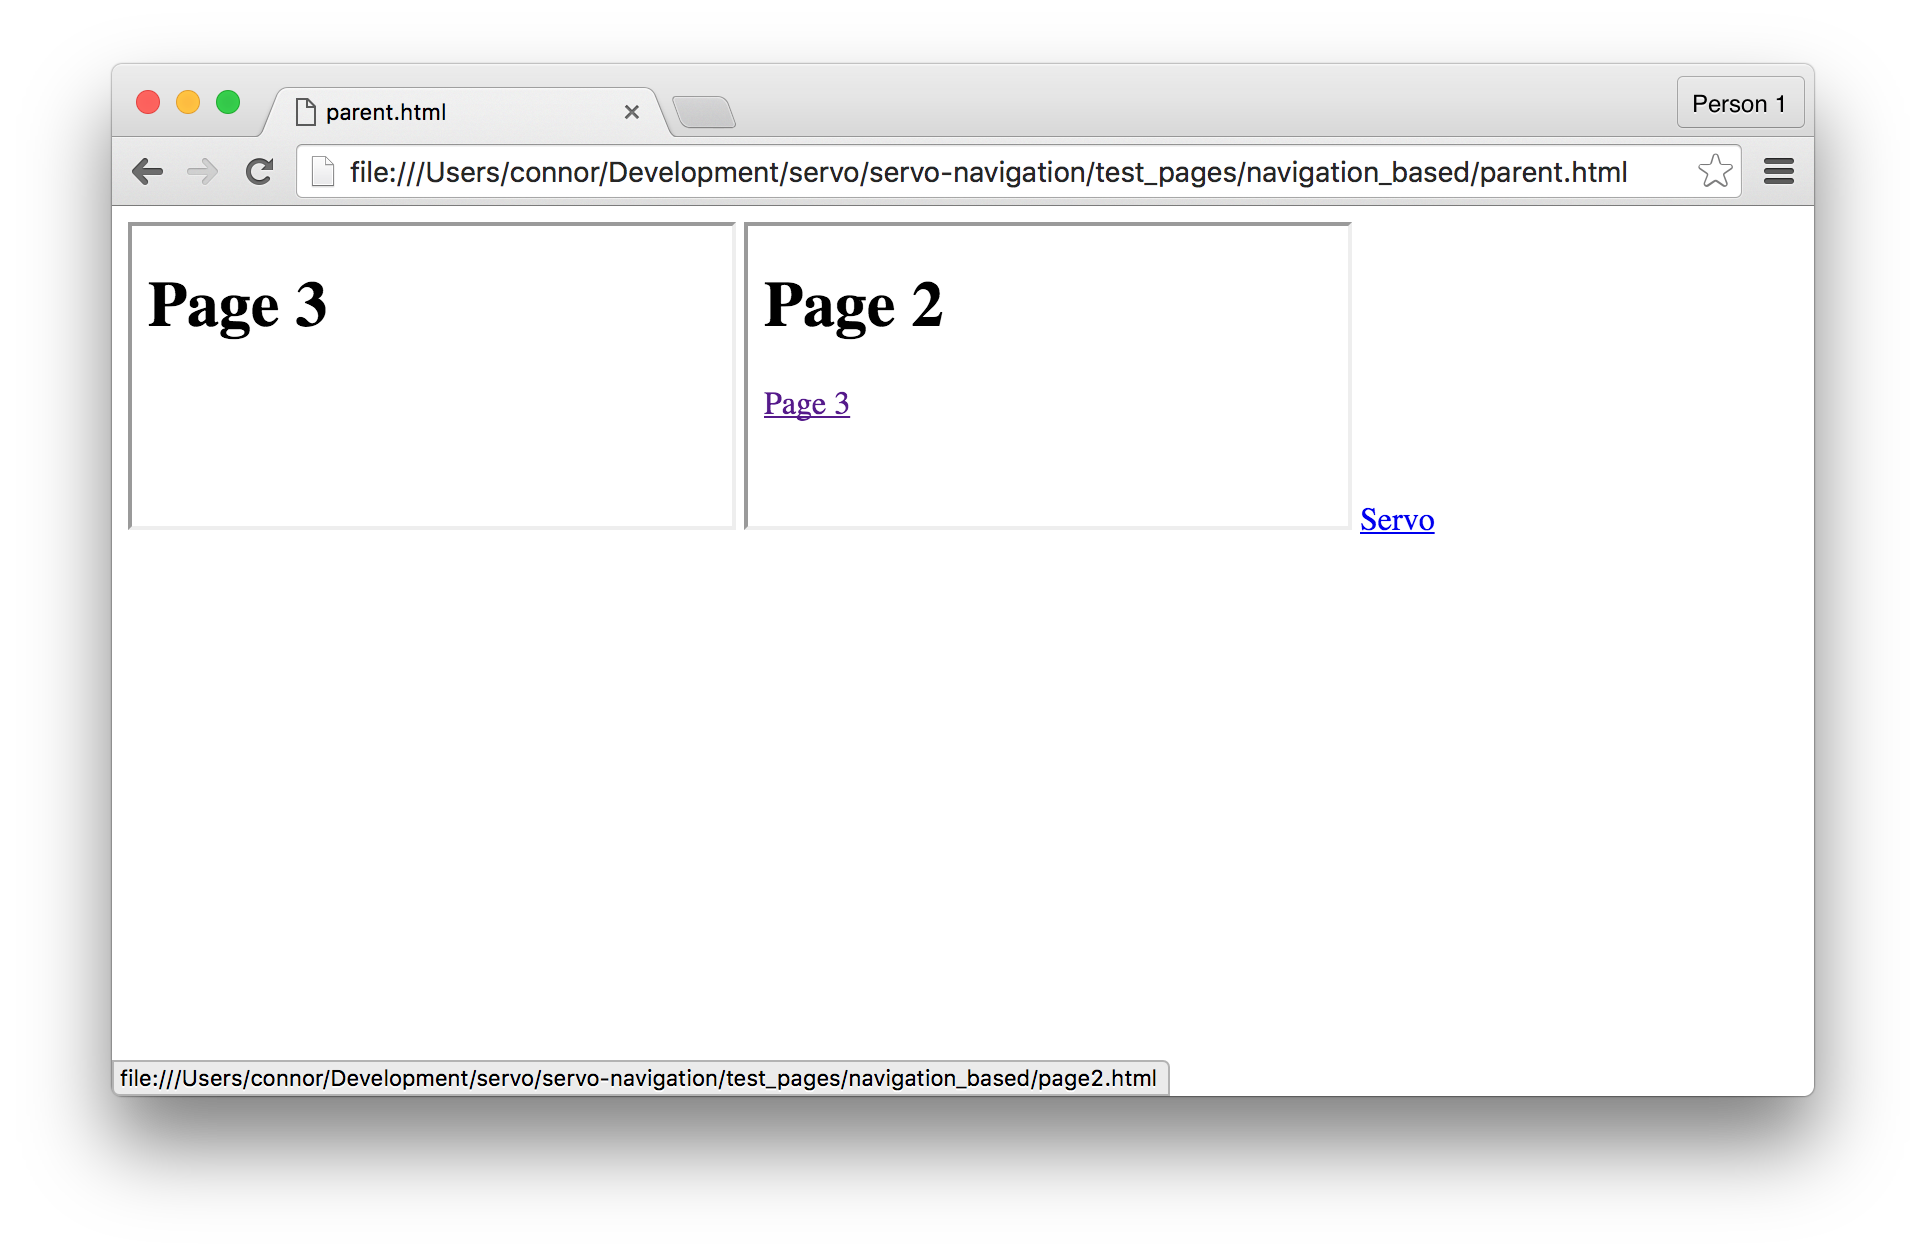
\includegraphics[width=.5\linewidth]{images/experiments/forwardback4/chrome/4.png}
    }~\raisebox{-.5\height}{
      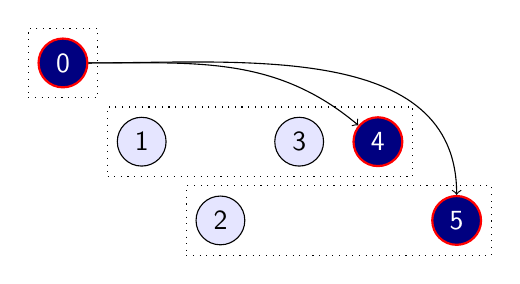
\begin{tikzpicture}
        \node[doc,active,fully](0) at (0,0){0};
        \node[doc](1) at (1,-1){1};
        \node[doc](2) at (2,-2){2};
        \node[doc](3) at (3,-1){3};
        \node[doc,active,fully](4) at (4,-1){4};
        \node[doc,jshactive,fully](5) at (5,-2){5};
        \node[draw,dotted,fit=(0)]{};
        \node[draw,dotted,fit=(1)(4)]{};
        \node[draw,dotted,fit=(2)(5)]{};
        \draw[->](0)to[out=0,in=140](4);
        \draw[->](0)to[out=0,in=90](5);
      \end{tikzpicture}
    }
    \caption{Navigate document $2$ to Page 2.}
  \end{figure}

  Navigate document $5$ to Page 3:
  \begin{figure}[H]
    \raisebox{-.5\height}{
      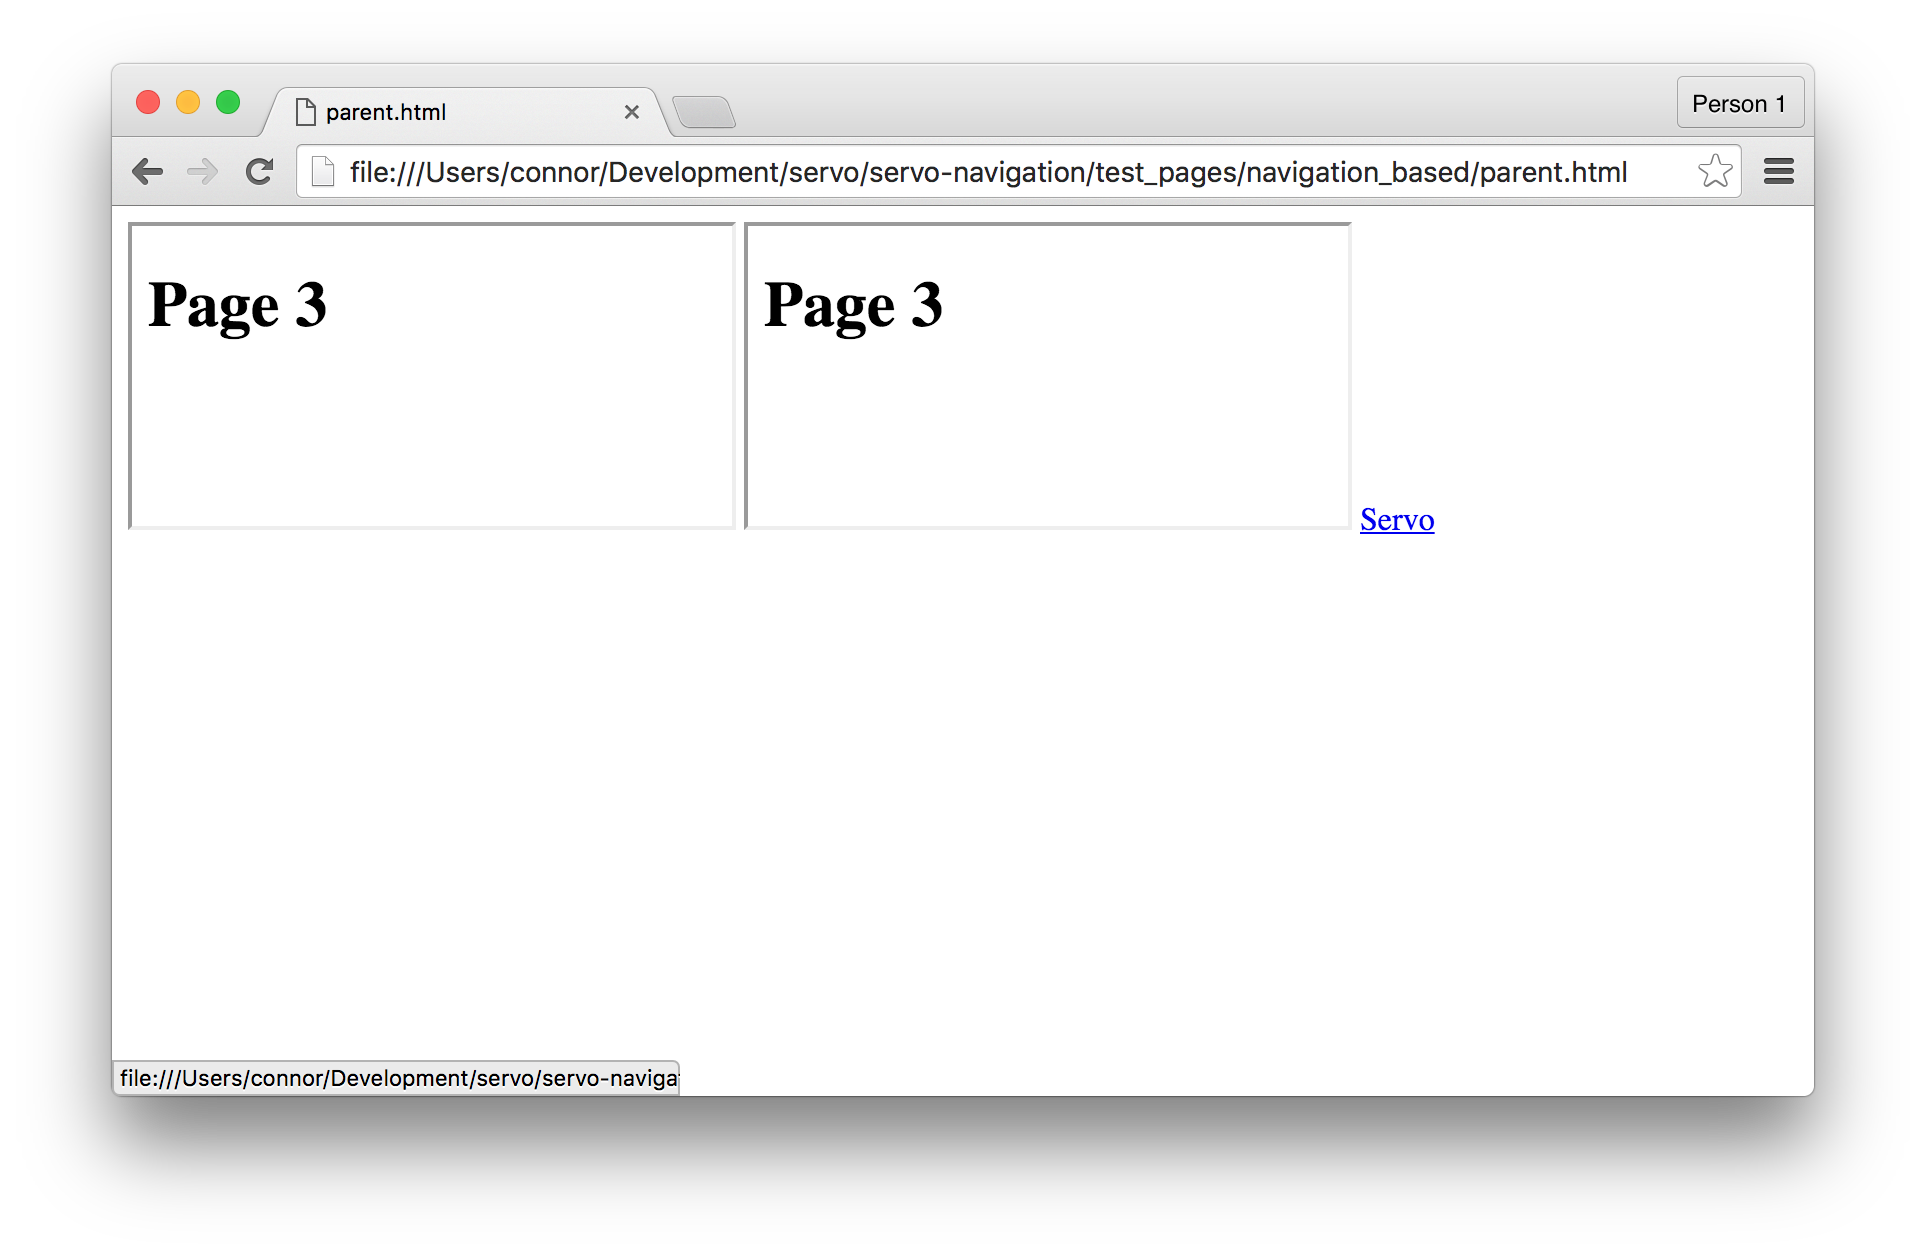
\includegraphics[width=.5\linewidth]{images/experiments/forwardback4/chrome/5.png}
    }~\raisebox{-.5\height}{
      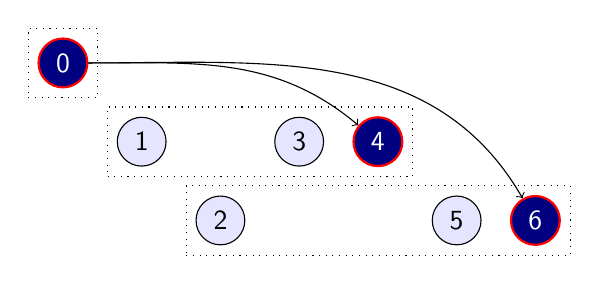
\begin{tikzpicture}
        \node[doc,active,fully](0) at (0,0){0};
        \node[doc](1) at (1,-1){1};
        \node[doc](2) at (2,-2){2};
        \node[doc](3) at (3,-1){3};
        \node[doc,active,fully](4) at (4,-1){4};
        \node[doc](5) at (5,-2){5};
        \node[doc,jshactive,fully](6) at (6,-2){6};
        \node[draw,dotted,fit=(0)]{};
        \node[draw,dotted,fit=(1)(4)]{};
        \node[draw,dotted,fit=(2)(6)]{};
        \draw[->](0)to[out=0,in=140](4);
        \draw[->](0)to[out=0,in=120](6);
      \end{tikzpicture}
    }
    \caption{Navigate document $5$ to Page 3.}
  \end{figure}

  \emph{$\aNH$ traverses the history by $-4$ to $\aNH'$}:
  \begin{figure}[H]
    \raisebox{-.5\height}{
      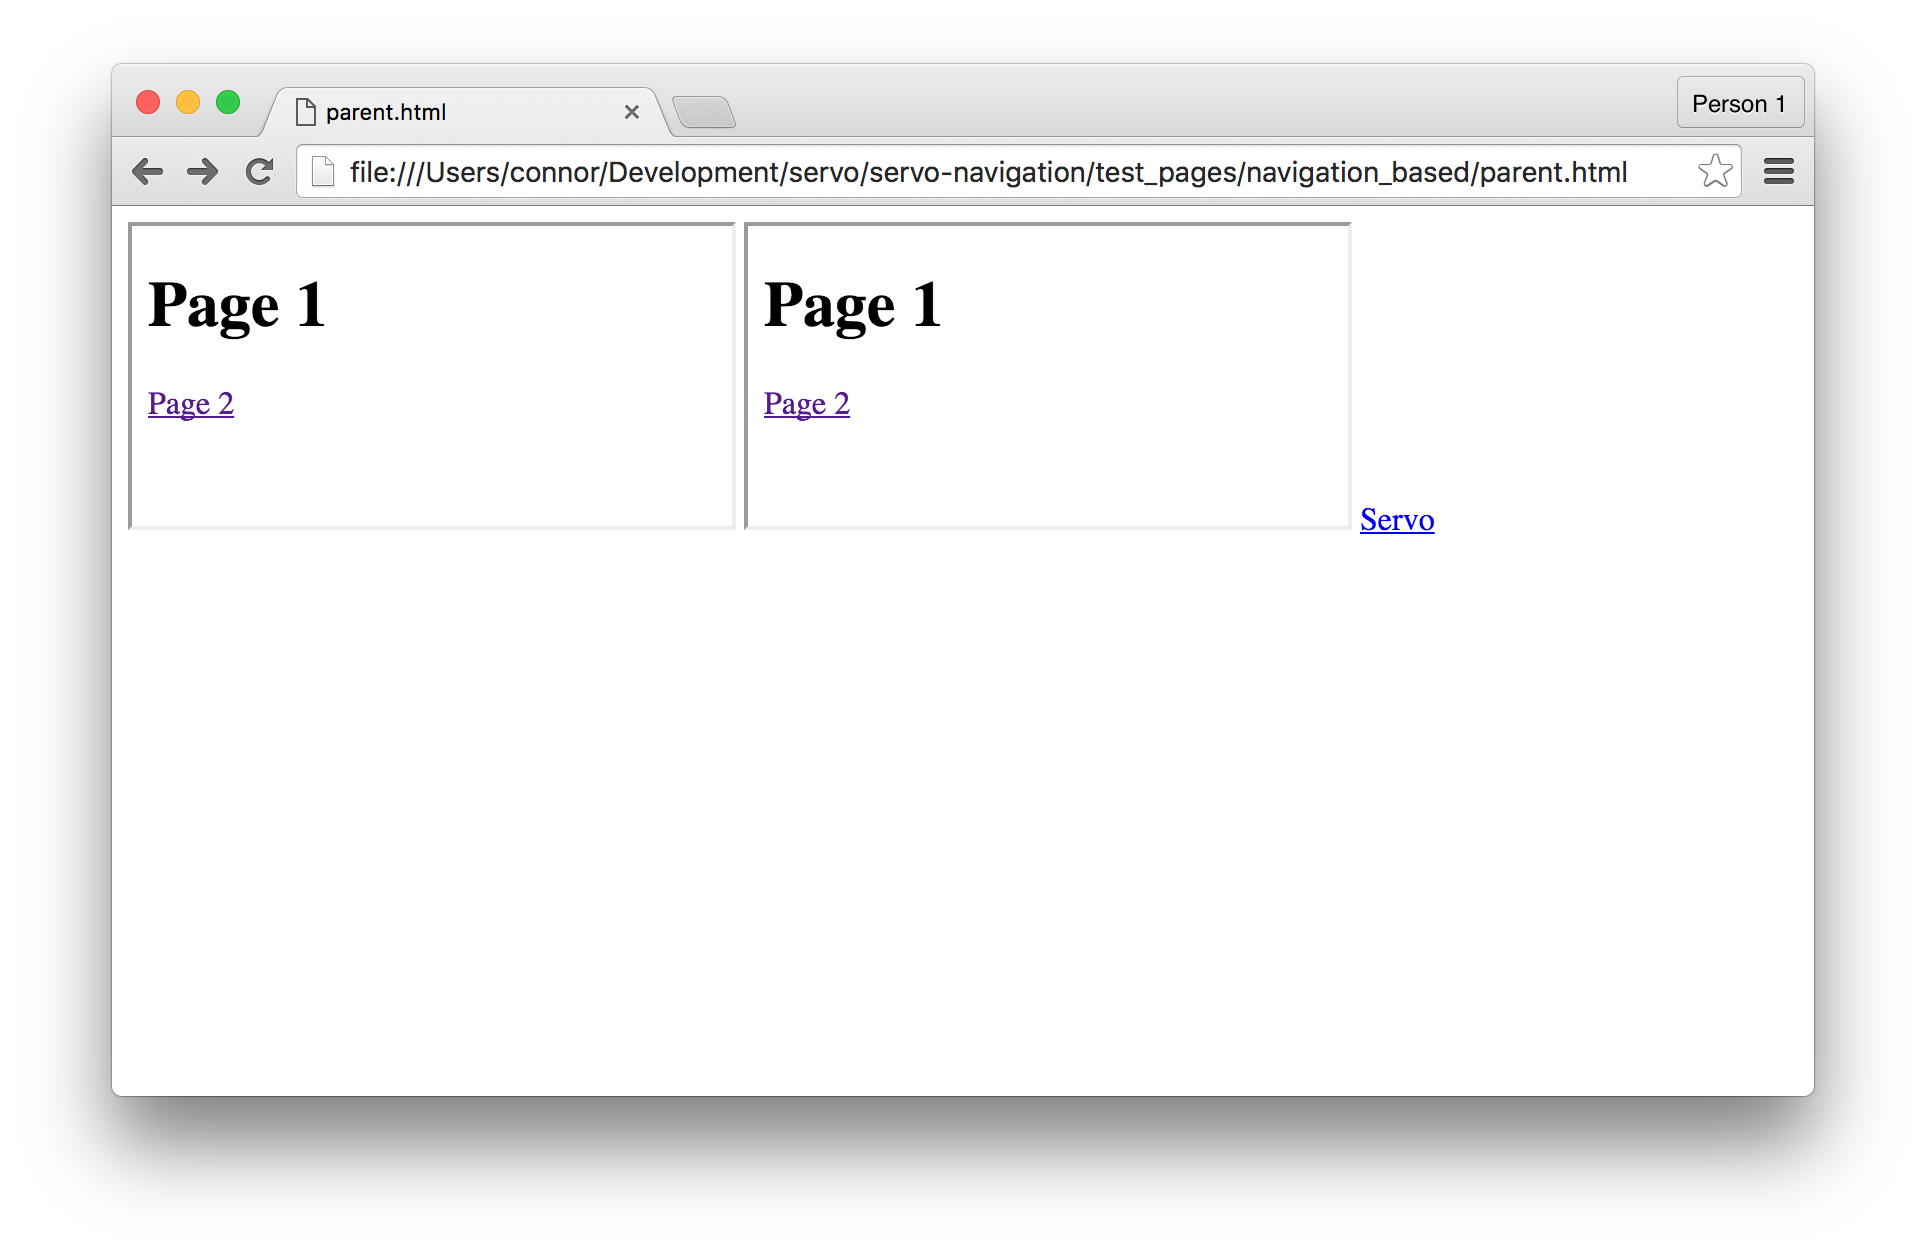
\includegraphics[width=.5\linewidth]{images/experiments/forwardback4/chrome/6.png}
    }~\raisebox{-.5\height}{
      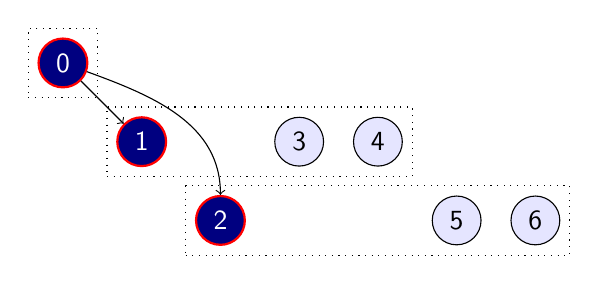
\begin{tikzpicture}
        \node[doc,active,fully](0) at (0,0){0};
        \node[doc,active,fully](1) at (1,-1){1};
        \node[doc,jshactive,fully](2) at (2,-2){2};
        \node[doc](3) at (3,-1){3};
        \node[doc](4) at (4,-1){4};
        \node[doc](5) at (5,-2){5};
        \node[doc](6) at (6,-2){6};
        \node[draw,dotted,fit=(0)]{};
        \node[draw,dotted,fit=(1)(4)]{};
        \node[draw,dotted,fit=(2)(6)]{};
        \draw[->](0)--(1);
        \draw[->](0)to[out=-20,in=90](2);
      \end{tikzpicture}
    }
    \caption{Traversal by $-4$.}
  \end{figure}

  \emph{$\aNH'$ traverses the history by $4$ to $\aNH''$}:
  \begin{figure}[H]
    \raisebox{-.5\height}{
      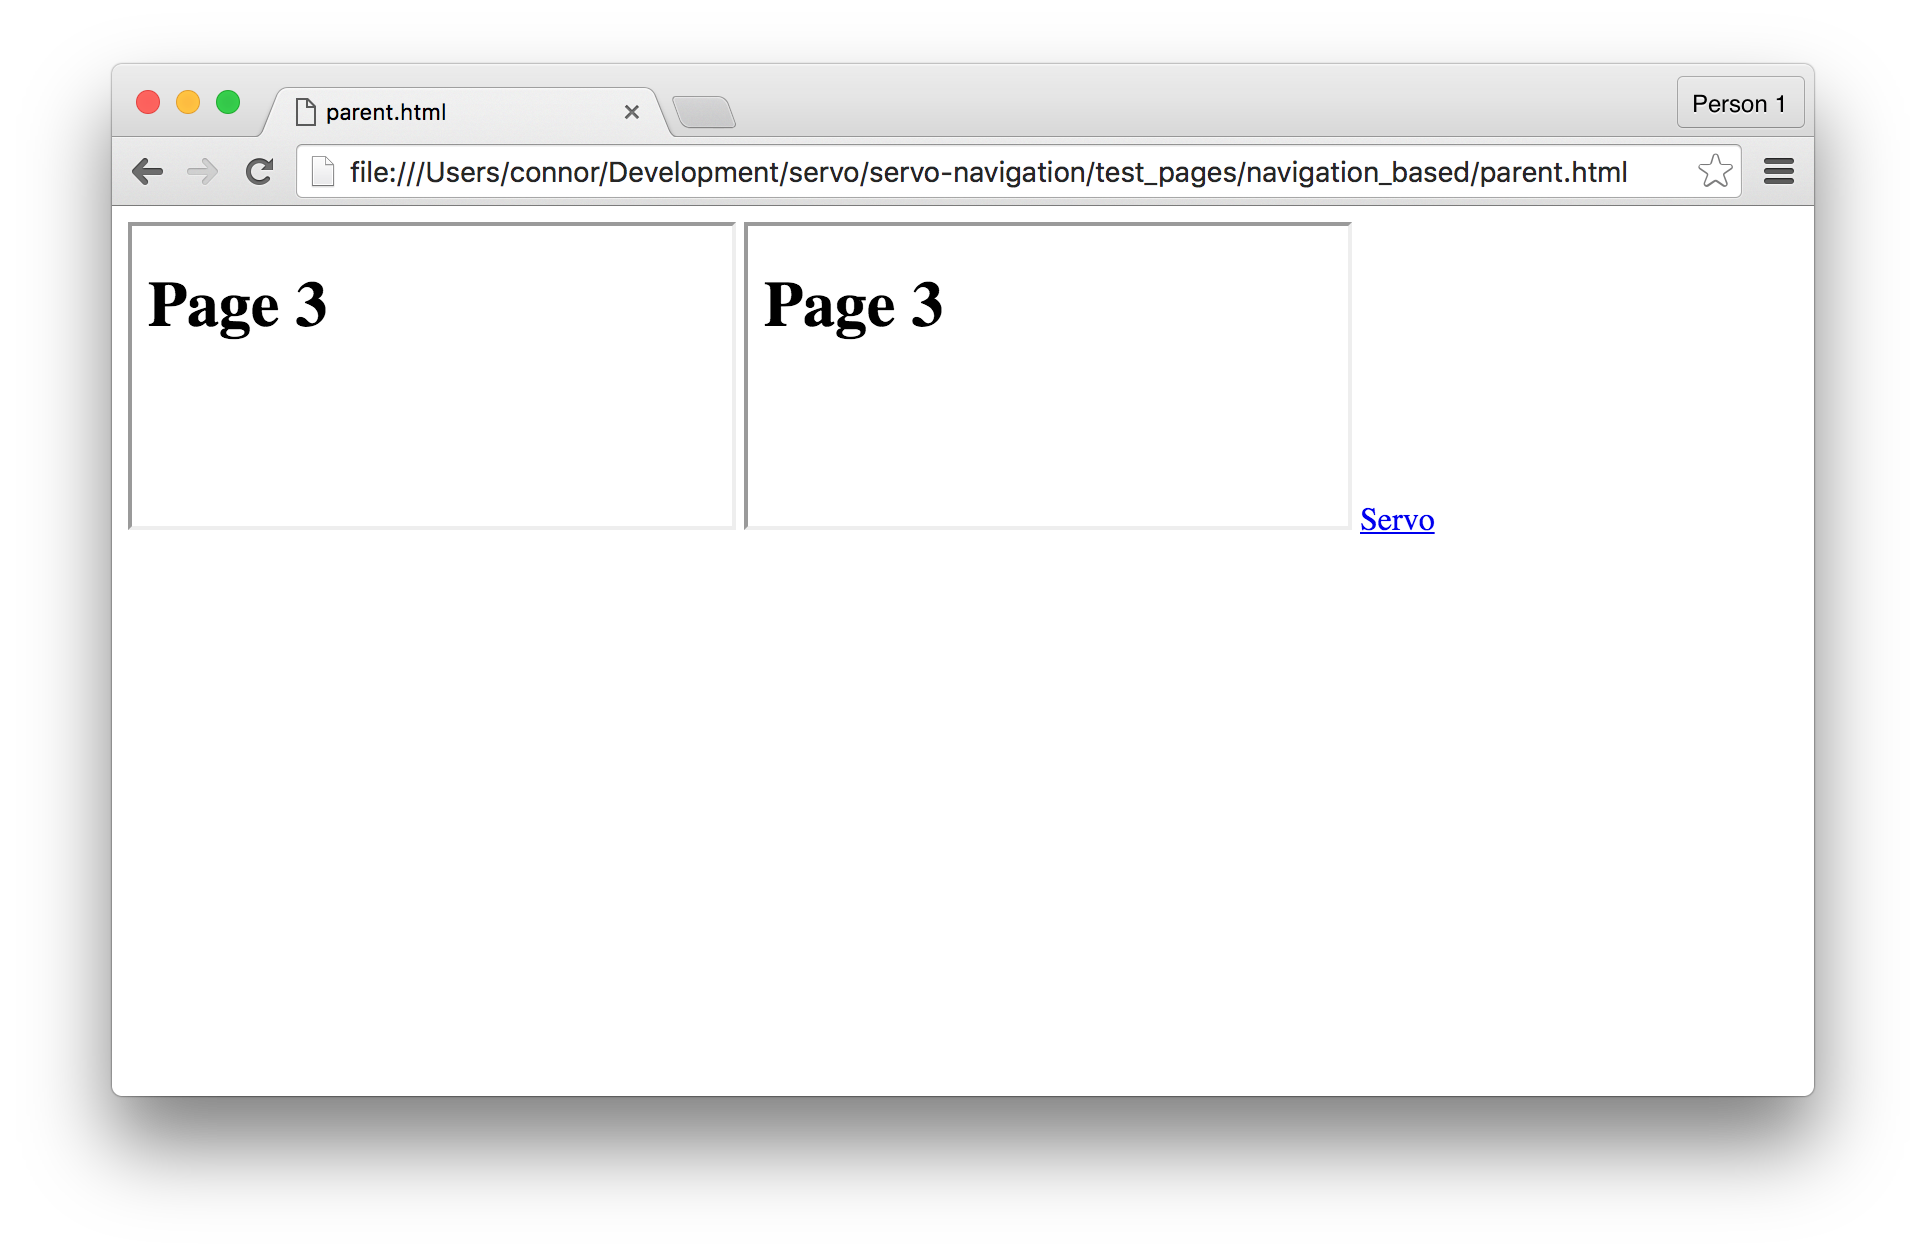
\includegraphics[width=.5\linewidth]{images/experiments/forwardback4/chrome/7.png}
    }~\raisebox{-.5\height}{
      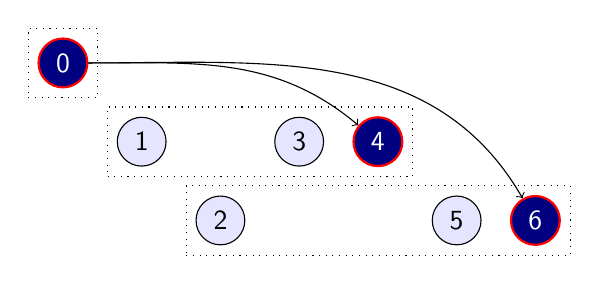
\begin{tikzpicture}
        \node[doc,active,fully](0) at (0,0){0};
        \node[doc](1) at (1,-1){1};
        \node[doc](2) at (2,-2){2};
        \node[doc](3) at (3,-1){3};
        \node[doc,active,fully](4) at (4,-1){4};
        \node[doc](5) at (5,-2){5};
        \node[doc,jshactive,fully](6) at (6,-2){6};
        \node[draw,dotted,fit=(0)]{};
        \node[draw,dotted,fit=(1)(4)]{};
        \node[draw,dotted,fit=(2)(6)]{};
        \draw[->](0)to[out=0,in=140](4);
        \draw[->](0)to[out=0,in=120](6);
      \end{tikzpicture}
    }
    \caption{Traversal by $4$.}
  \end{figure}

  These results in Chrome satisfy Goal~\ref{goal:homomorphism}.
\end{experiment}

\begin{experiment}
  In this experiment $pushState$ and $replaceState$ traversals are tested against Goal~\ref{goal:homomorphism}.

  Firefox:
  \begin{figure}[H]
    \raisebox{-.5\height}{
      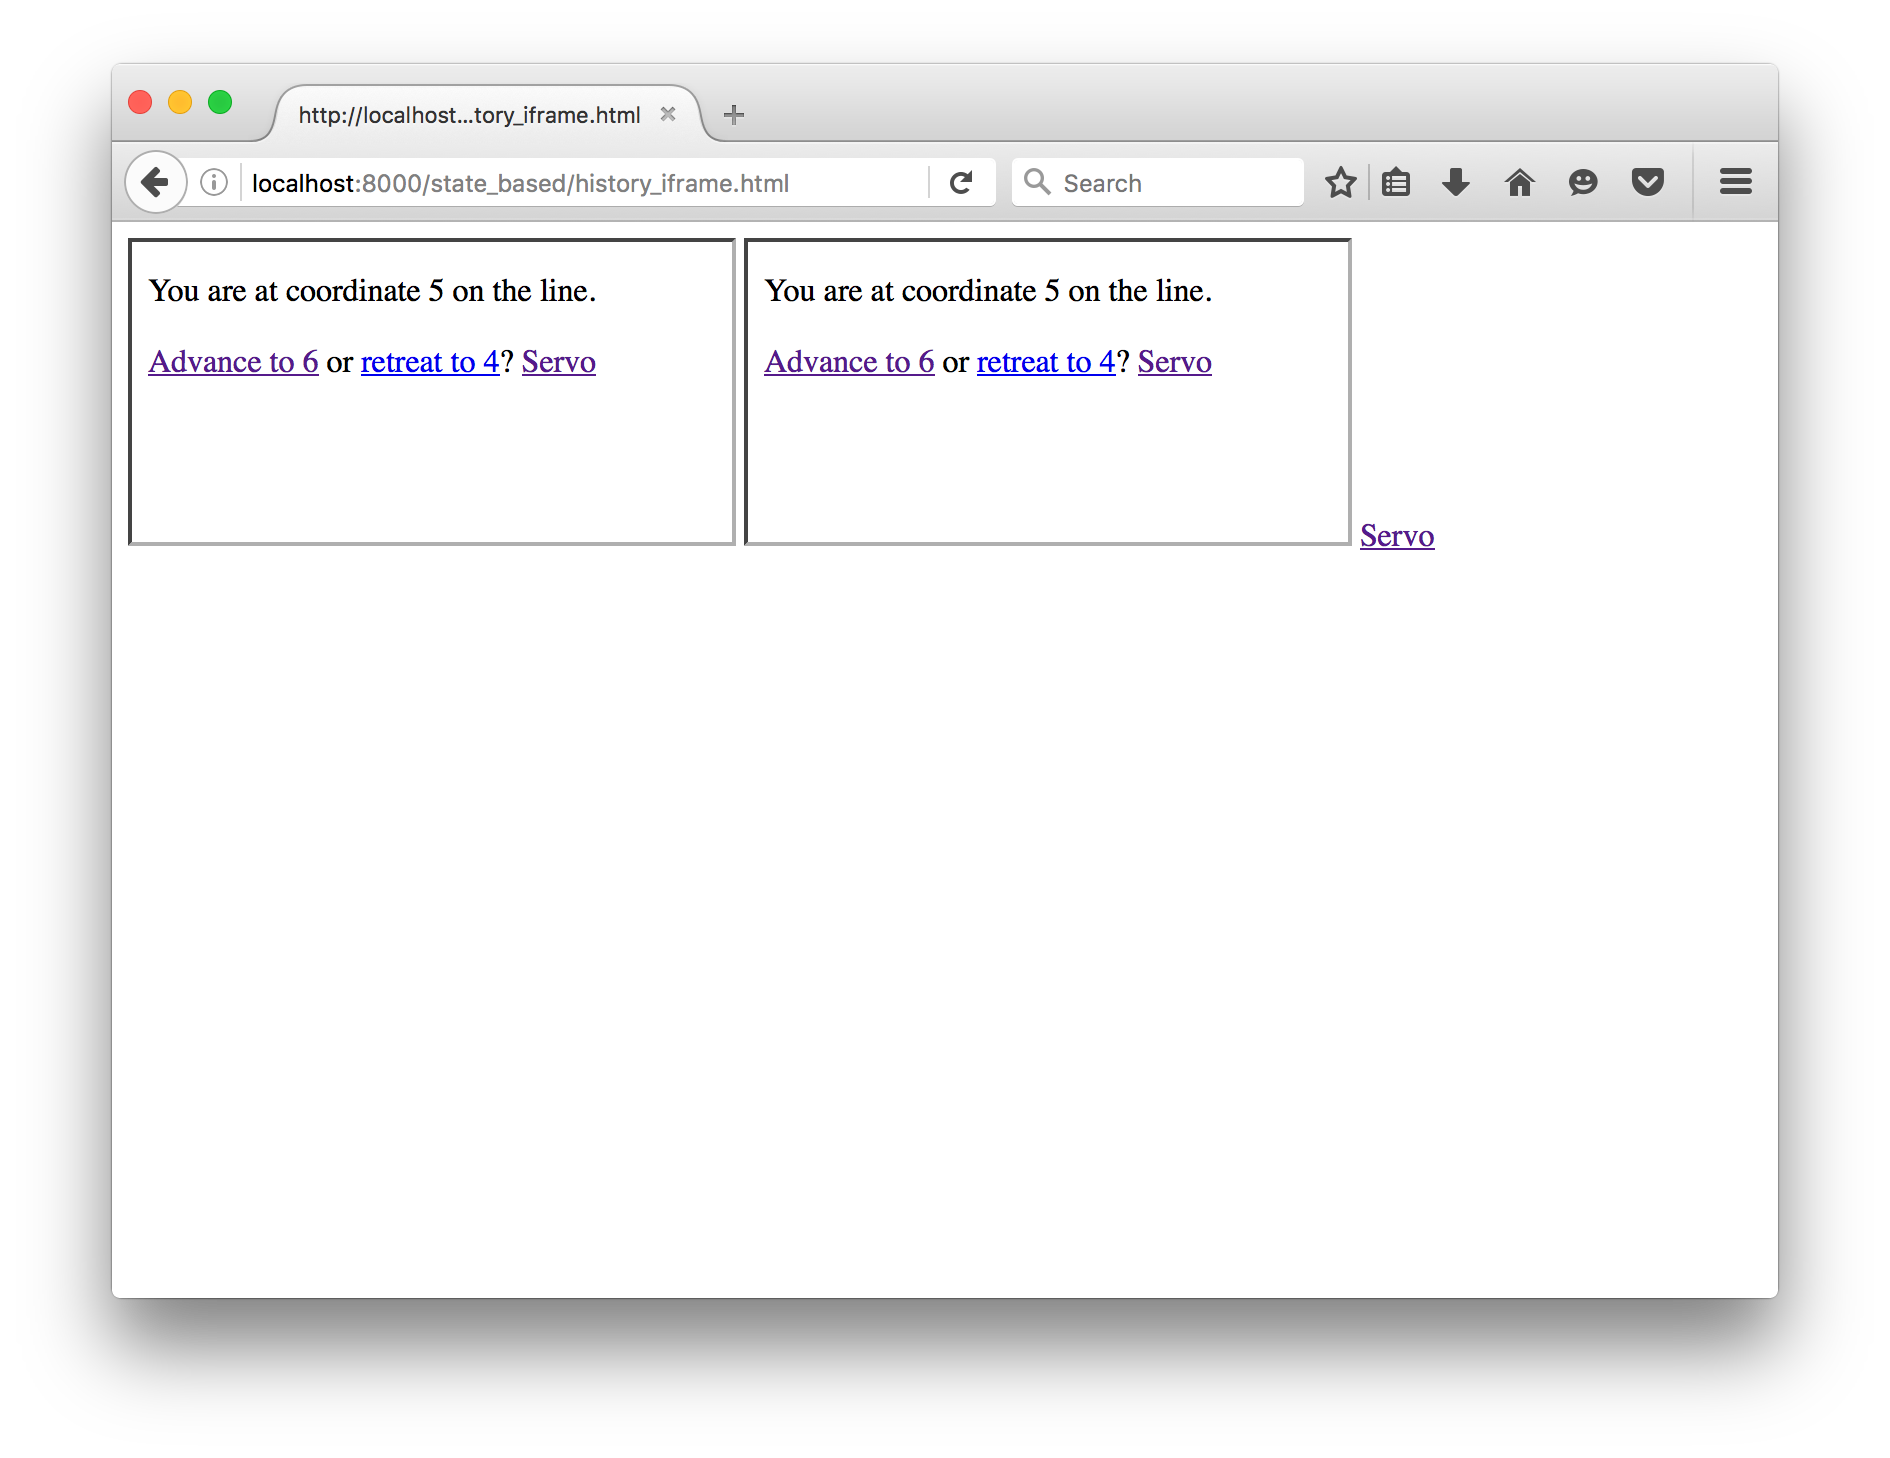
\includegraphics[width=.5\linewidth]{images/experiments/forwardback4state/firefox/1.png}%
    }~\raisebox{-.5\height}{
      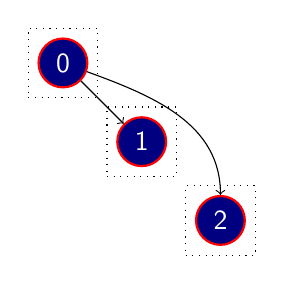
\begin{tikzpicture}
        \node[doc,active,fully](0) at (0,0){0};
        \node[doc,active,fully](1) at (1,-1){1};
        \node[doc,jshactive,fully](2) at (2,-2){2};
        \node[draw,dotted,fit=(0)]{};
        \node[draw,dotted,fit=(1)]{};
        \node[draw,dotted,fit=(2)]{};
        \draw[->](0)--(1);
        \draw[->](0)to[out=-20,in=90](2);
      \end{tikzpicture}
    }
    \caption{Initial State}
  \end{figure}

  Advance document 1 to $6$:
  \begin{figure}[H]
    \raisebox{-.5\height}{
      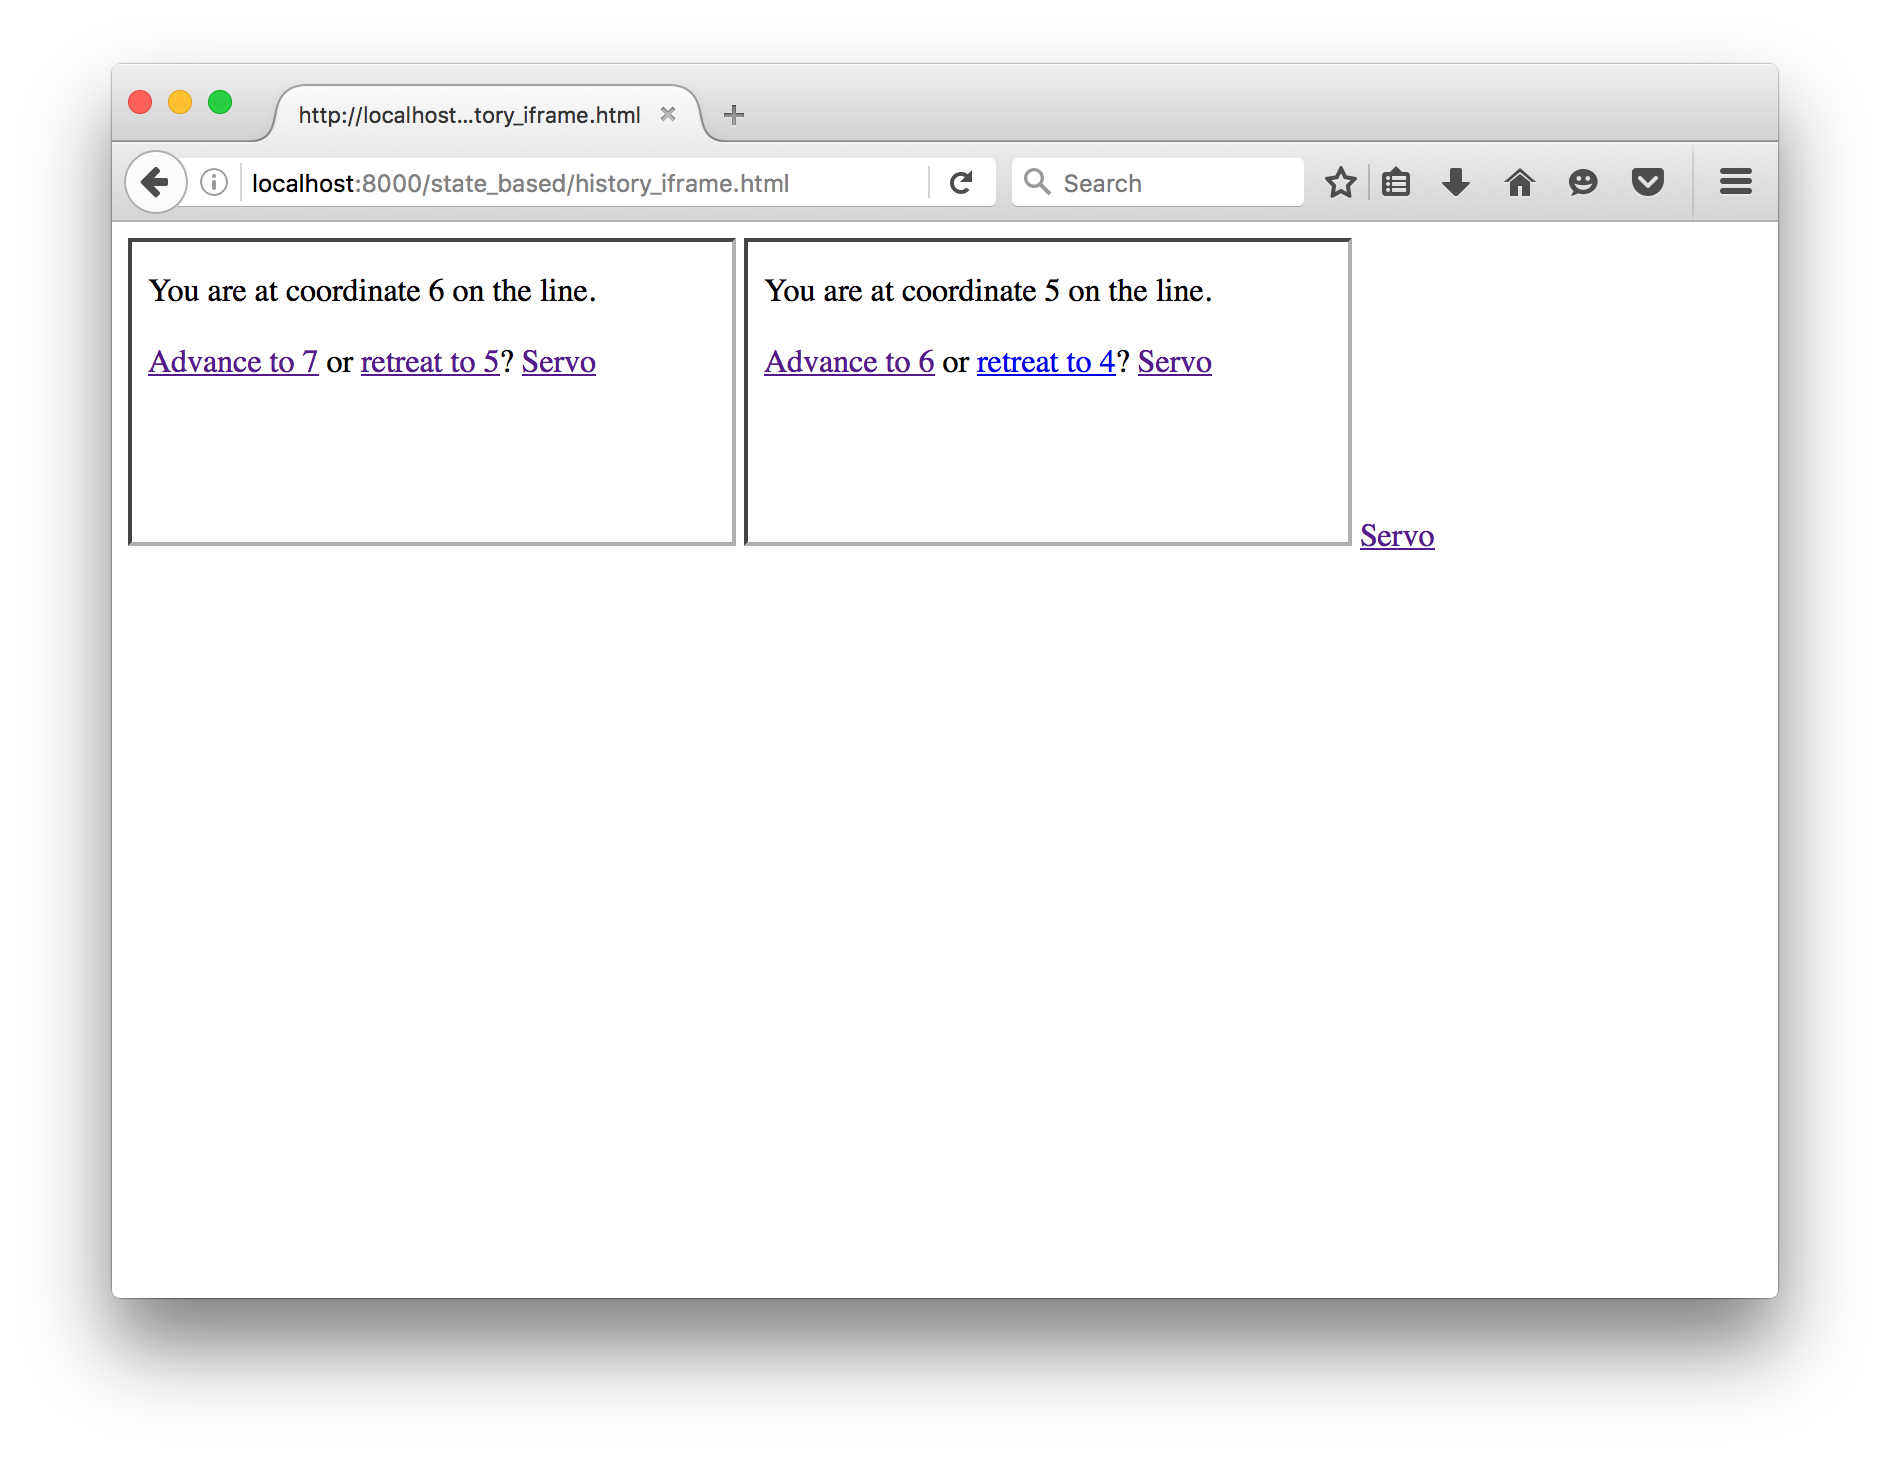
\includegraphics[width=.5\linewidth]{images/experiments/forwardback4state/firefox/2.png}%
    }~\raisebox{-.5\height}{
      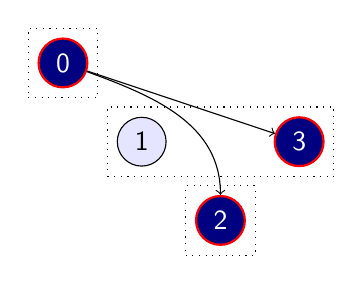
\begin{tikzpicture}
        \node[doc,active,fully](0) at (0,0){0};
        \node[doc](1) at (1,-1){1};
        \node[doc,active,fully](2) at (2,-2){2};
        \node[doc,jshactive,fully](3) at (3,-1){3};
        \node[draw,dotted,fit=(0)]{};
        \node[draw,dotted,fit=(1)(3)]{};
        \node[draw,dotted,fit=(2)]{};
        \draw[->](0)--(3);
        \draw[->](0)to[out=-20,in=90](2);
      \end{tikzpicture}
    }
    \caption{Advance document 1 to $6$}
  \end{figure}

  Advance document 3 to $7$:
  \begin{figure}[H]
    \raisebox{-.5\height}{
      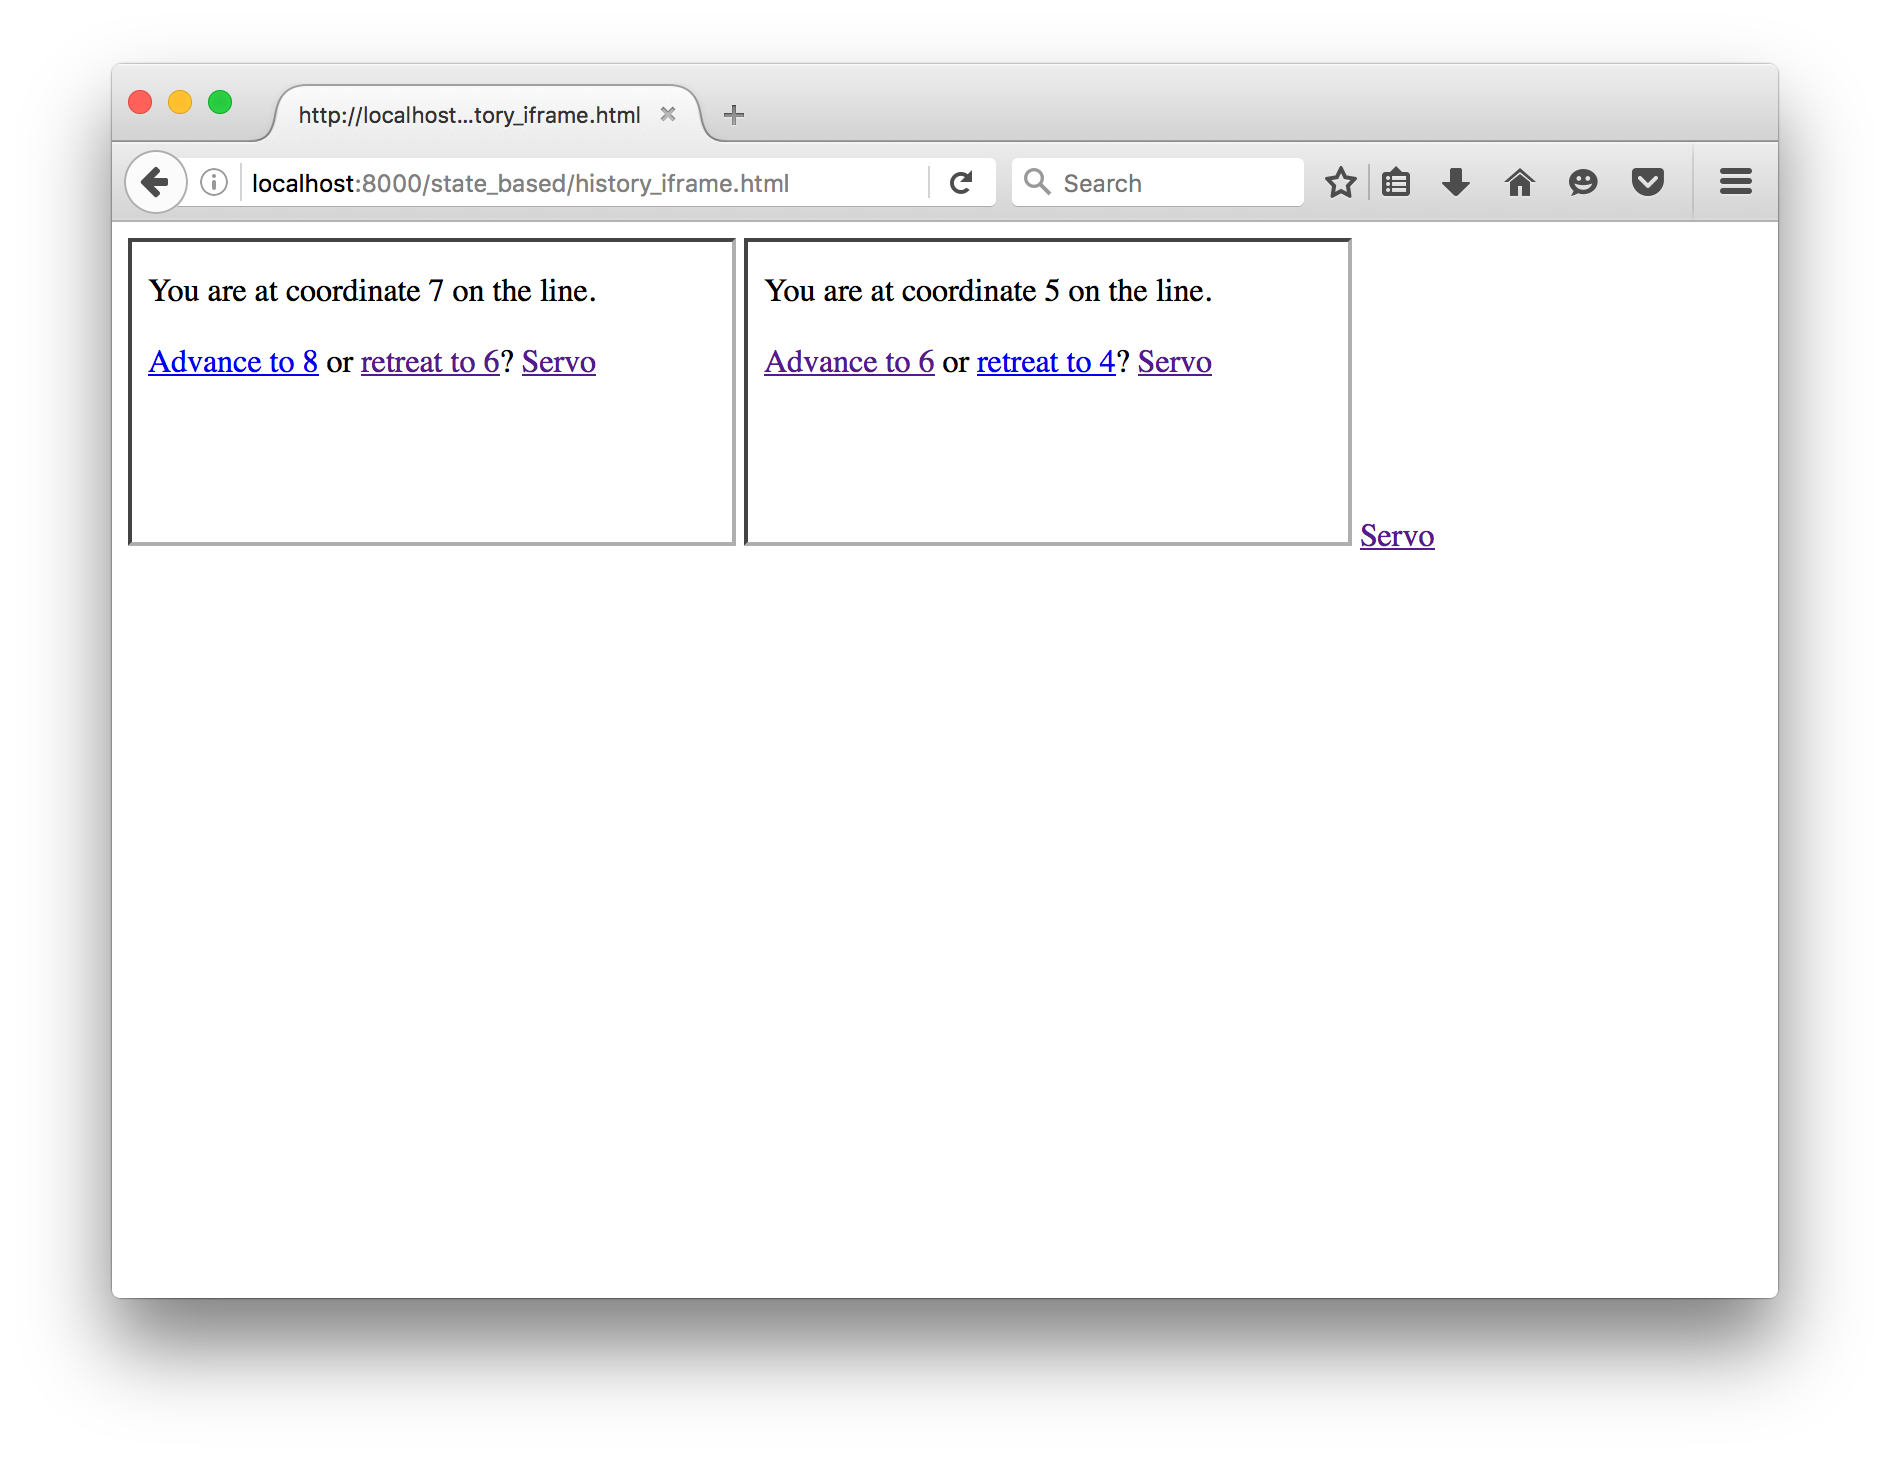
\includegraphics[width=.5\linewidth]{images/experiments/forwardback4state/firefox/3.png}%
    }~\raisebox{-.5\height}{
      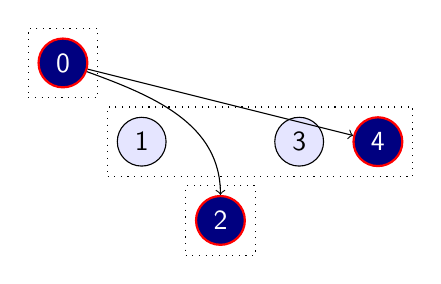
\begin{tikzpicture}
        \node[doc,active,fully](0) at (0,0){0};
        \node[doc](1) at (1,-1){1};
        \node[doc,active,fully](2) at (2,-2){2};
        \node[doc](3) at (3,-1){3};
        \node[doc,jshactive,fully](4) at (4,-1){4};
        \node[draw,dotted,fit=(0)]{};
        \node[draw,dotted,fit=(1)(4)]{};
        \node[draw,dotted,fit=(2)]{};
        \draw[->](0)--(4);
        \draw[->](0)to[out=-20,in=90](2);
      \end{tikzpicture}
    }
    \caption{Advance document 3 to $7$}
  \end{figure}

  Advance document 2 to $6$:
  \begin{figure}[H]
    \raisebox{-.5\height}{
      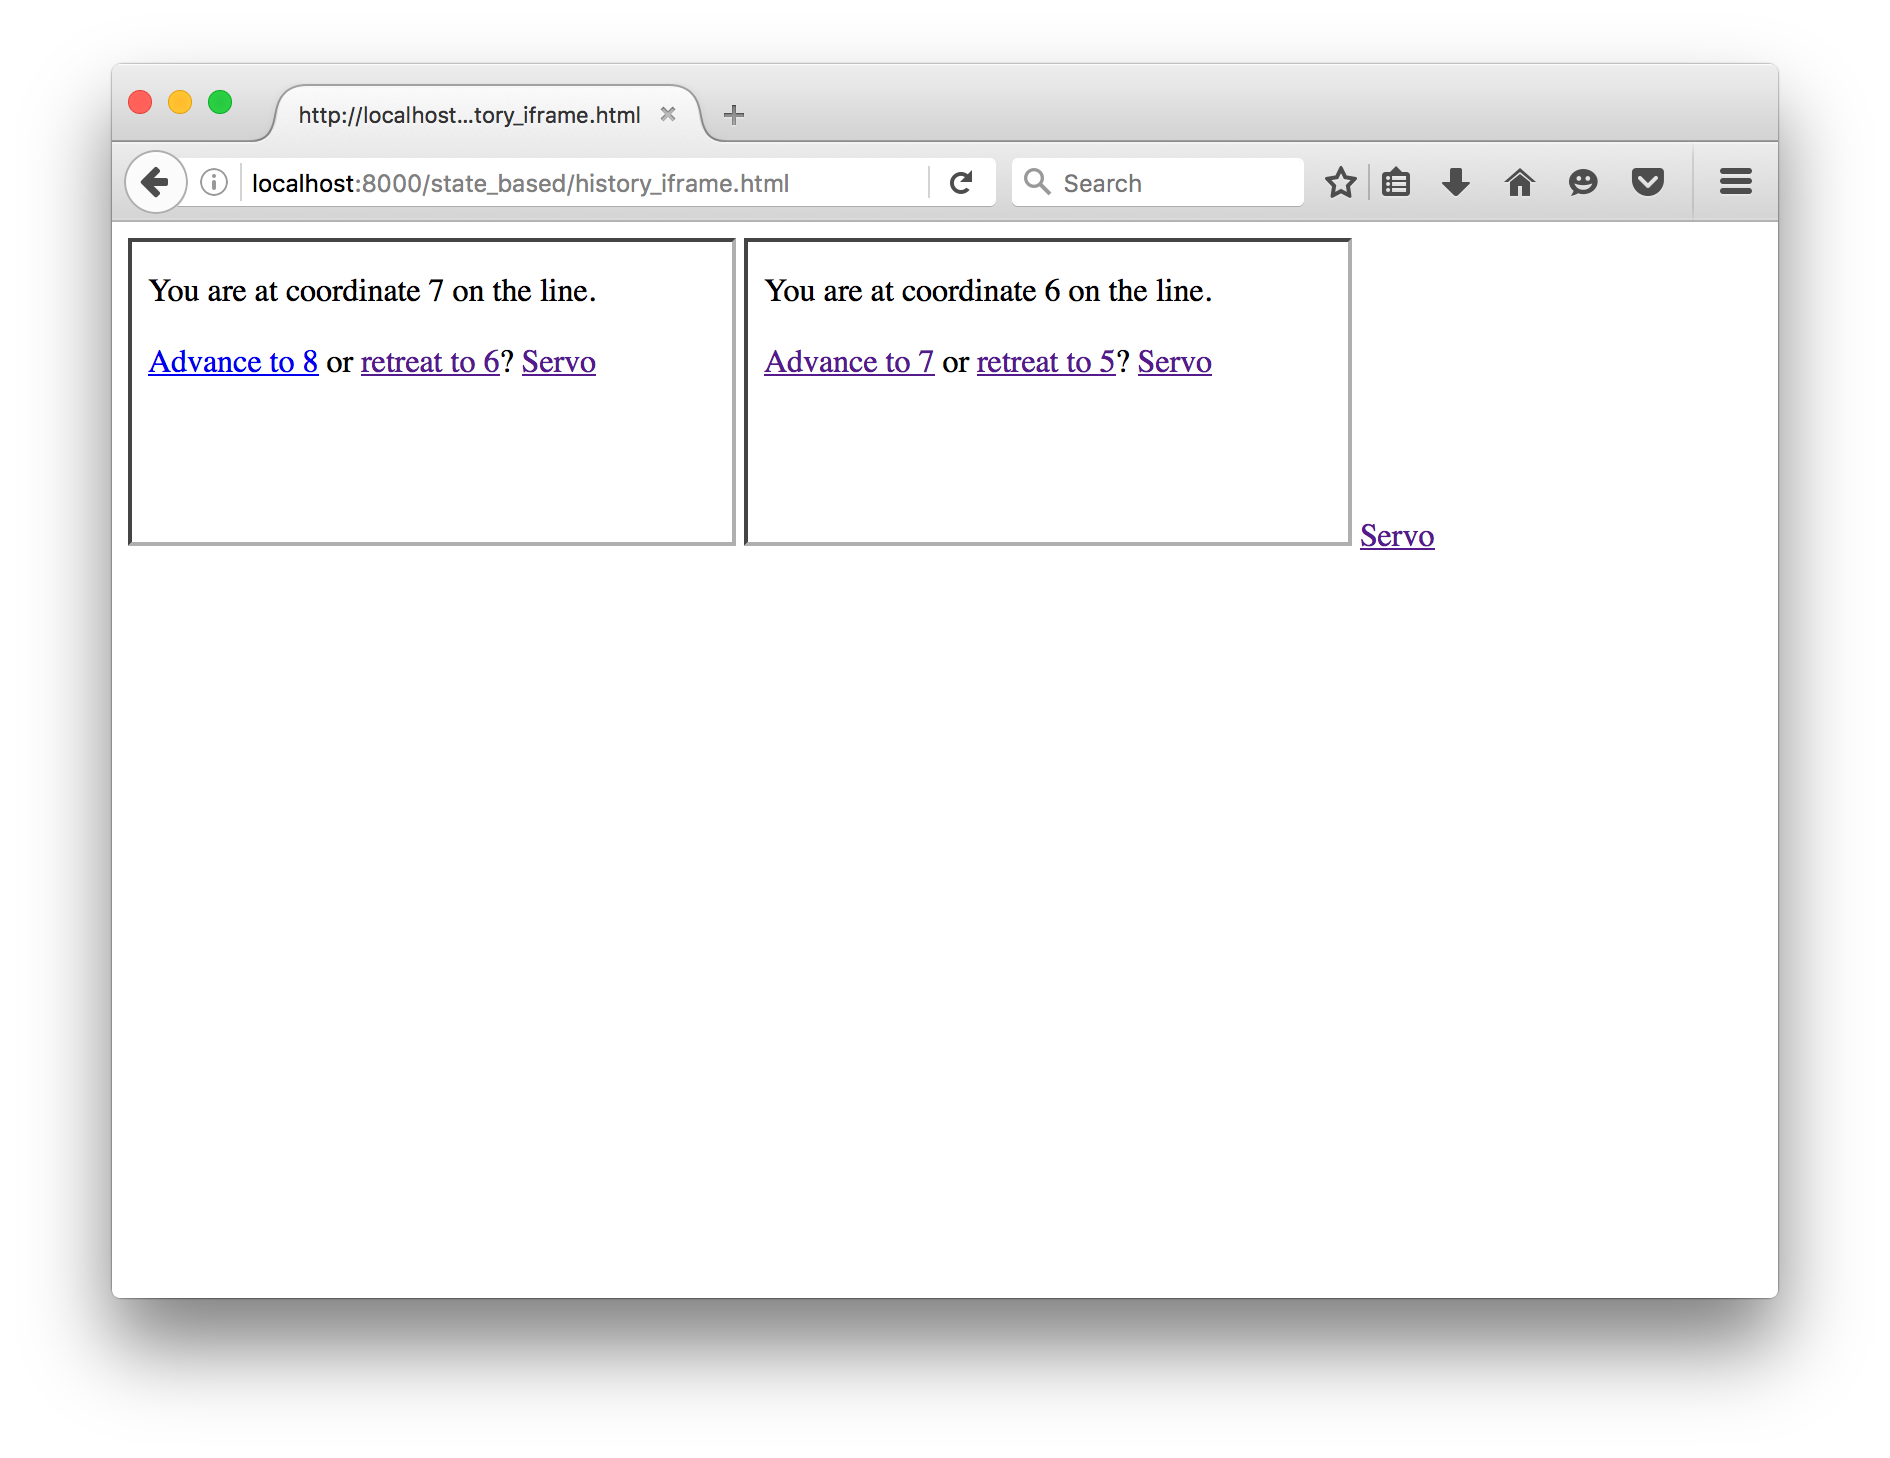
\includegraphics[width=.5\linewidth]{images/experiments/forwardback4state/firefox/4.png}%
    }~\raisebox{-.5\height}{
      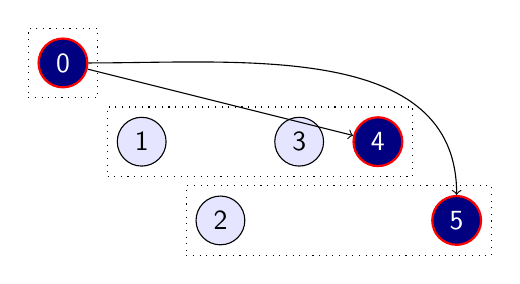
\begin{tikzpicture}
        \node[doc,active,fully](0) at (0,0){0};
        \node[doc](1) at (1,-1){1};
        \node[doc](2) at (2,-2){2};
        \node[doc](3) at (3,-1){3};
        \node[doc,active,fully](4) at (4,-1){4};
        \node[doc,jshactive,fully](5) at (5,-2){5};
        \node[draw,dotted,fit=(0)]{};
        \node[draw,dotted,fit=(1)(4)]{};
        \node[draw,dotted,fit=(2)(5)]{};
        \draw[->](0)--(4);
        \draw[->](0)to[out=0,in=90](5);
      \end{tikzpicture}
    }
    \caption{Advance $document 2$ to $6$}
  \end{figure}

  Advance $document 2$ to $7$:
  \begin{figure}[H]
    \raisebox{-.5\height}{
      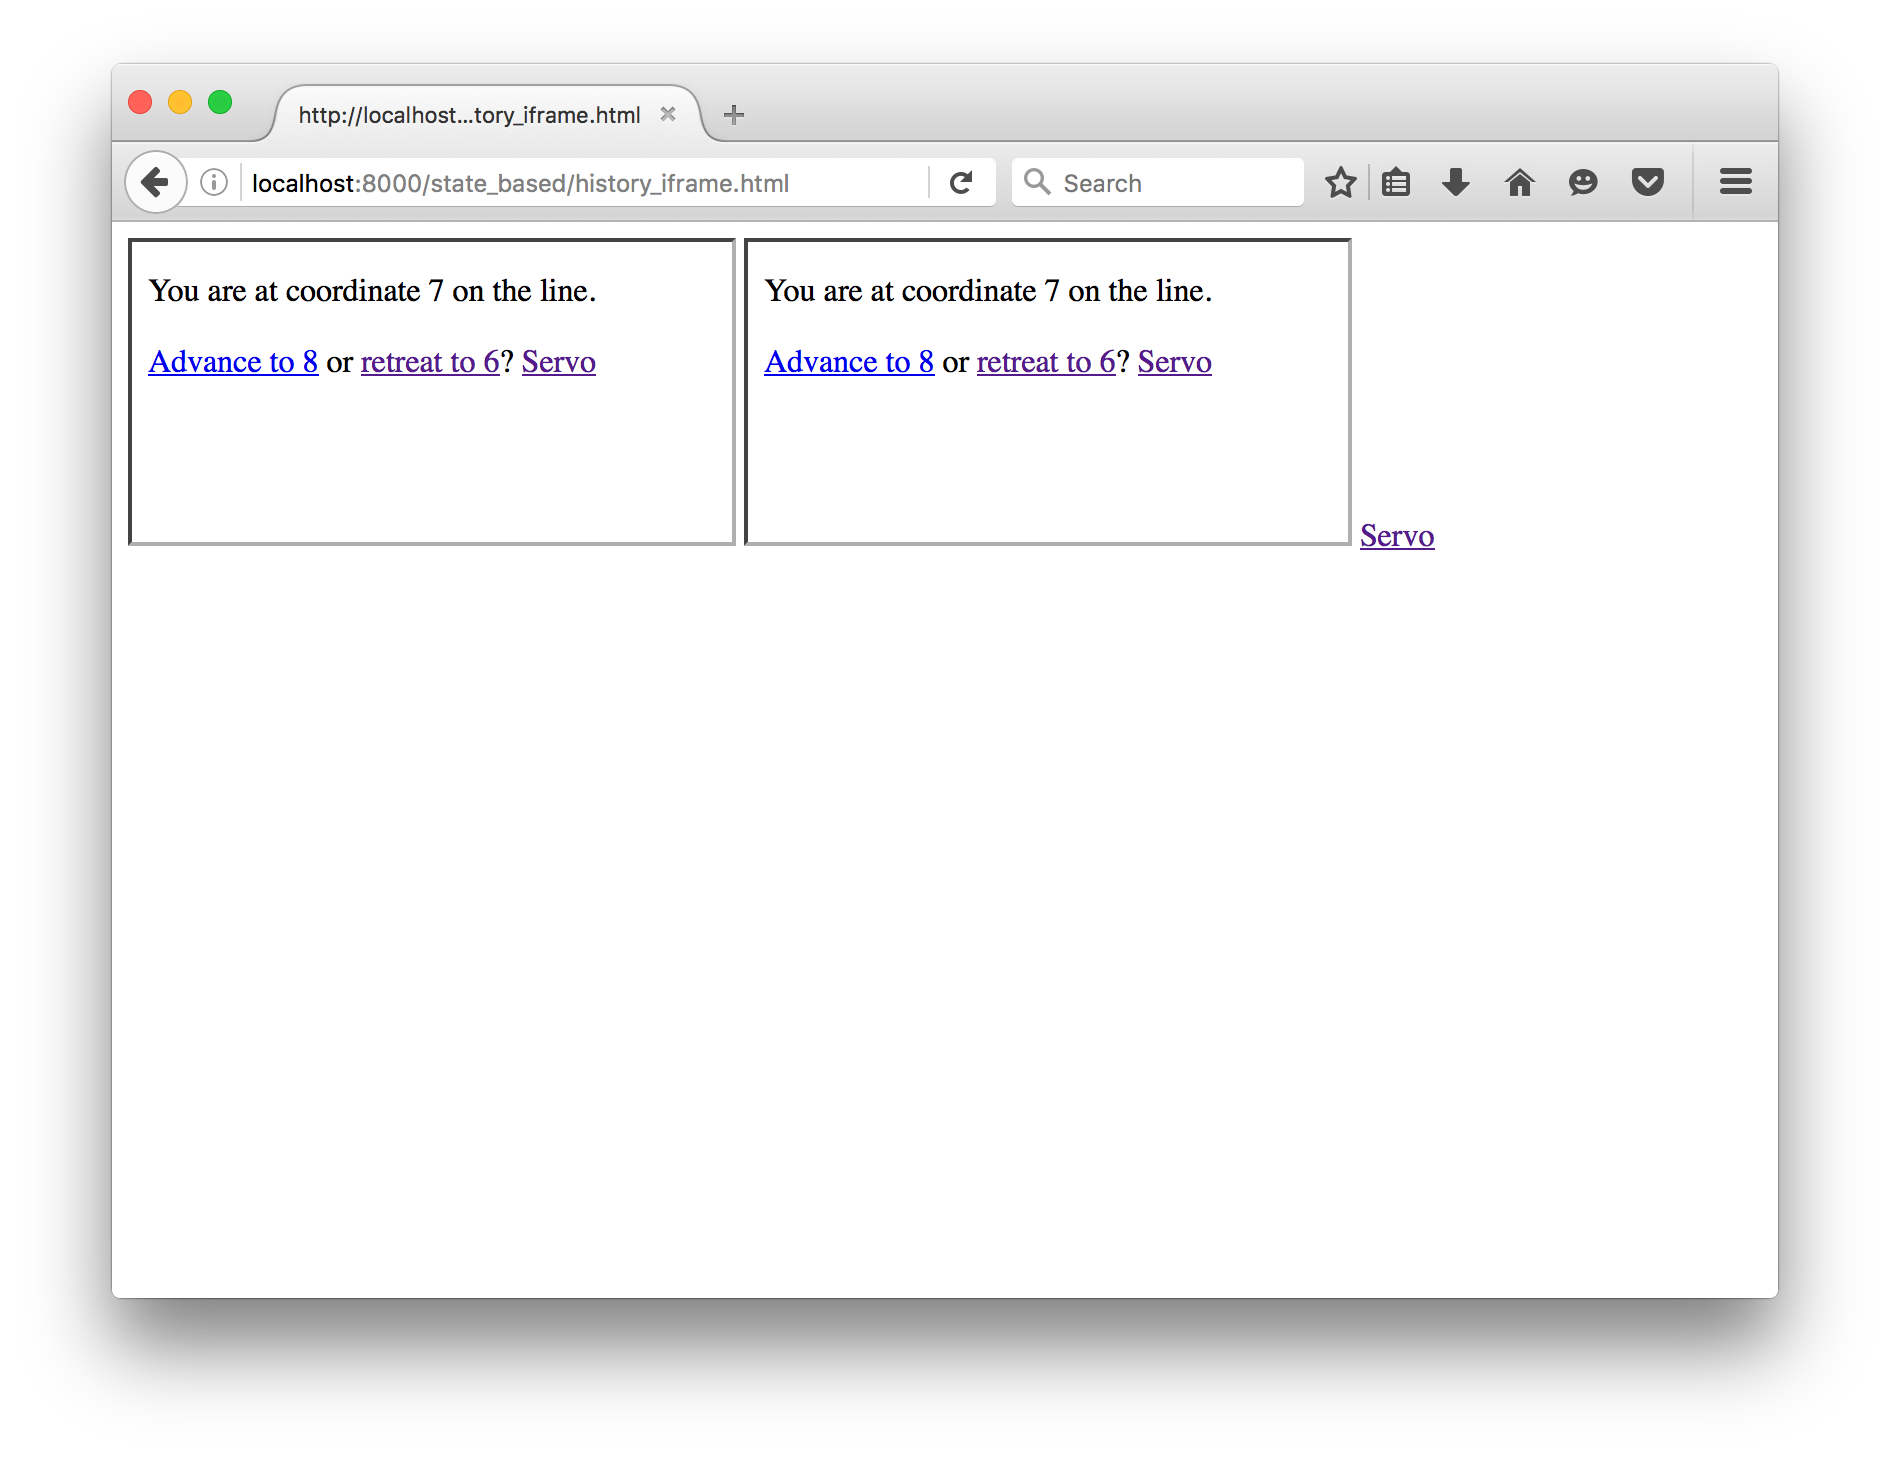
\includegraphics[width=.5\linewidth]{images/experiments/forwardback4state/firefox/5.png}%
    }~\raisebox{-.5\height}{
      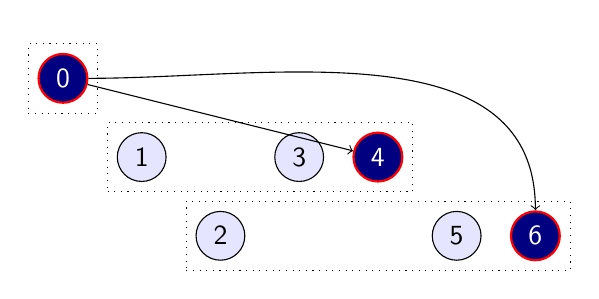
\begin{tikzpicture}
        \node[doc,active,fully](0) at (0,0){0};
        \node[doc](1) at (1,-1){1};
        \node[doc](2) at (2,-2){2};
        \node[doc](3) at (3,-1){3};
        \node[doc,active,fully](4) at (4,-1){4};
        \node[doc](5) at (5,-2){5};
        \node[doc,jshactive,fully](6) at (6,-2){6};
        \node[draw,dotted,fit=(0)]{};
        \node[draw,dotted,fit=(1)(4)]{};
        \node[draw,dotted,fit=(2)(6)]{};
        \draw[->](0)--(4);
        \draw[->](0)to[out=0,in=90](6);
      \end{tikzpicture}
    }
    \caption{Advance document 2 to $7$}
  \end{figure}

  Traverse $\aNH$ by $-4$:
  \begin{figure}[H]
    \raisebox{-.5\height}{
      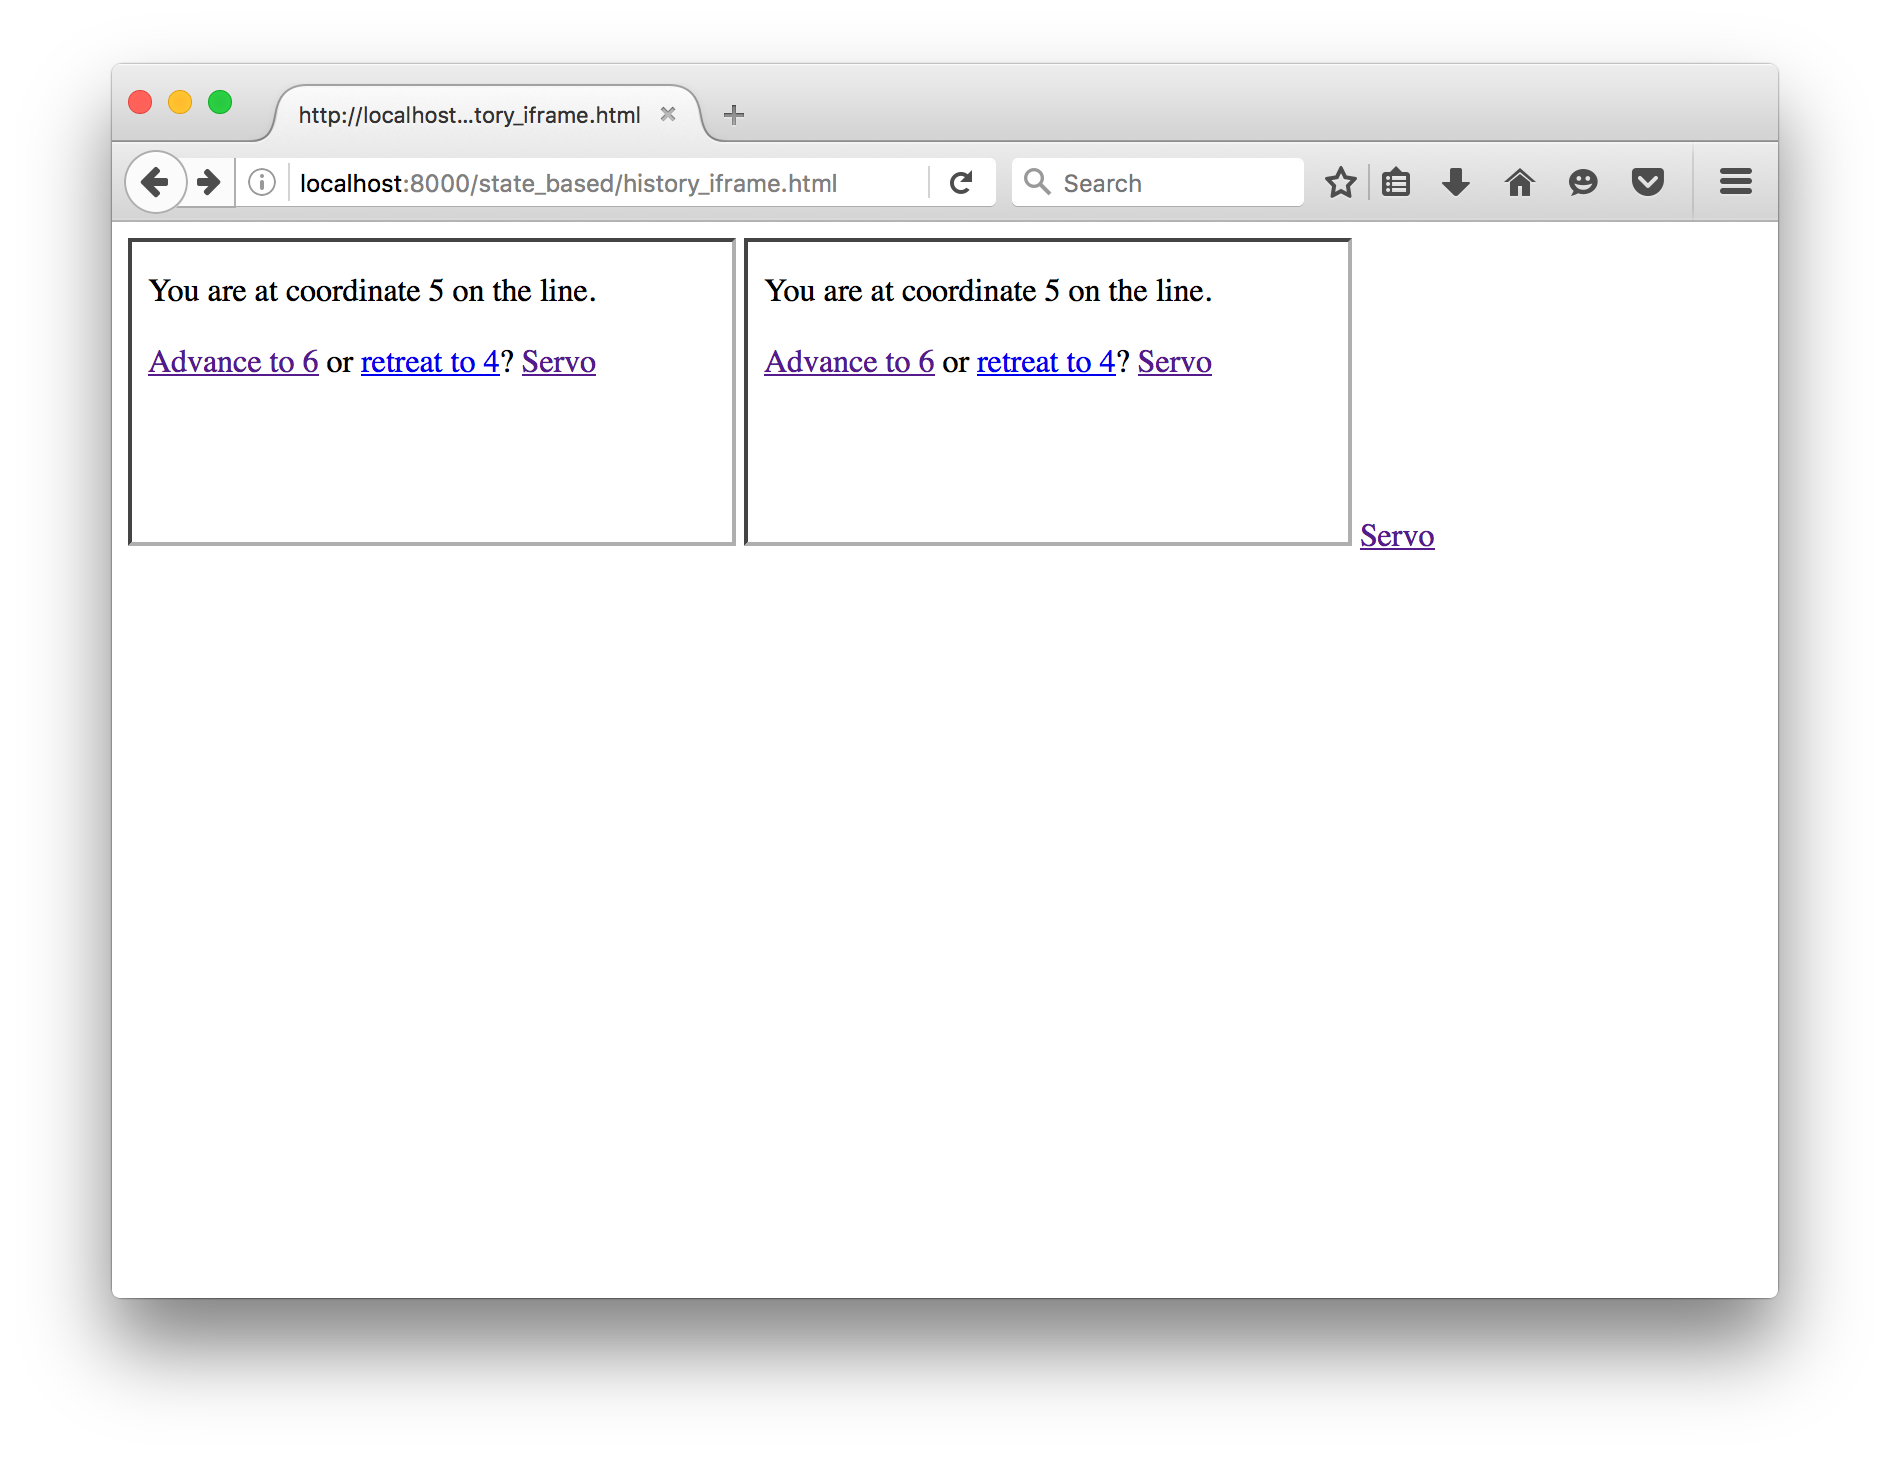
\includegraphics[width=.5\linewidth]{images/experiments/forwardback4state/firefox/6.png}%
    }~\raisebox{-.5\height}{
      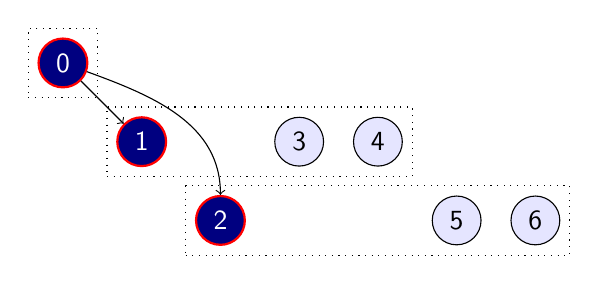
\begin{tikzpicture}
        \node[doc,active,fully](0) at (0,0){0};
        \node[doc,active,fully](1) at (1,-1){1};
        \node[doc,jshactive,fully](2) at (2,-2){2};
        \node[doc](3) at (3,-1){3};
        \node[doc](4) at (4,-1){4};
        \node[doc](5) at (5,-2){5};
        \node[doc](6) at (6,-2){6};
        \node[draw,dotted,fit=(0)]{};
        \node[draw,dotted,fit=(1)(4)]{};
        \node[draw,dotted,fit=(2)(6)]{};
        \draw[->](0)--(1);
        \draw[->](0)to[out=-20,in=90](2);
      \end{tikzpicture}
    }
    \caption{Traverse $\aNH$ by $-4$}
  \end{figure}

  Traverse $\aNH$ by $4$:
  \begin{figure}[H]
    \raisebox{-.5\height}{
      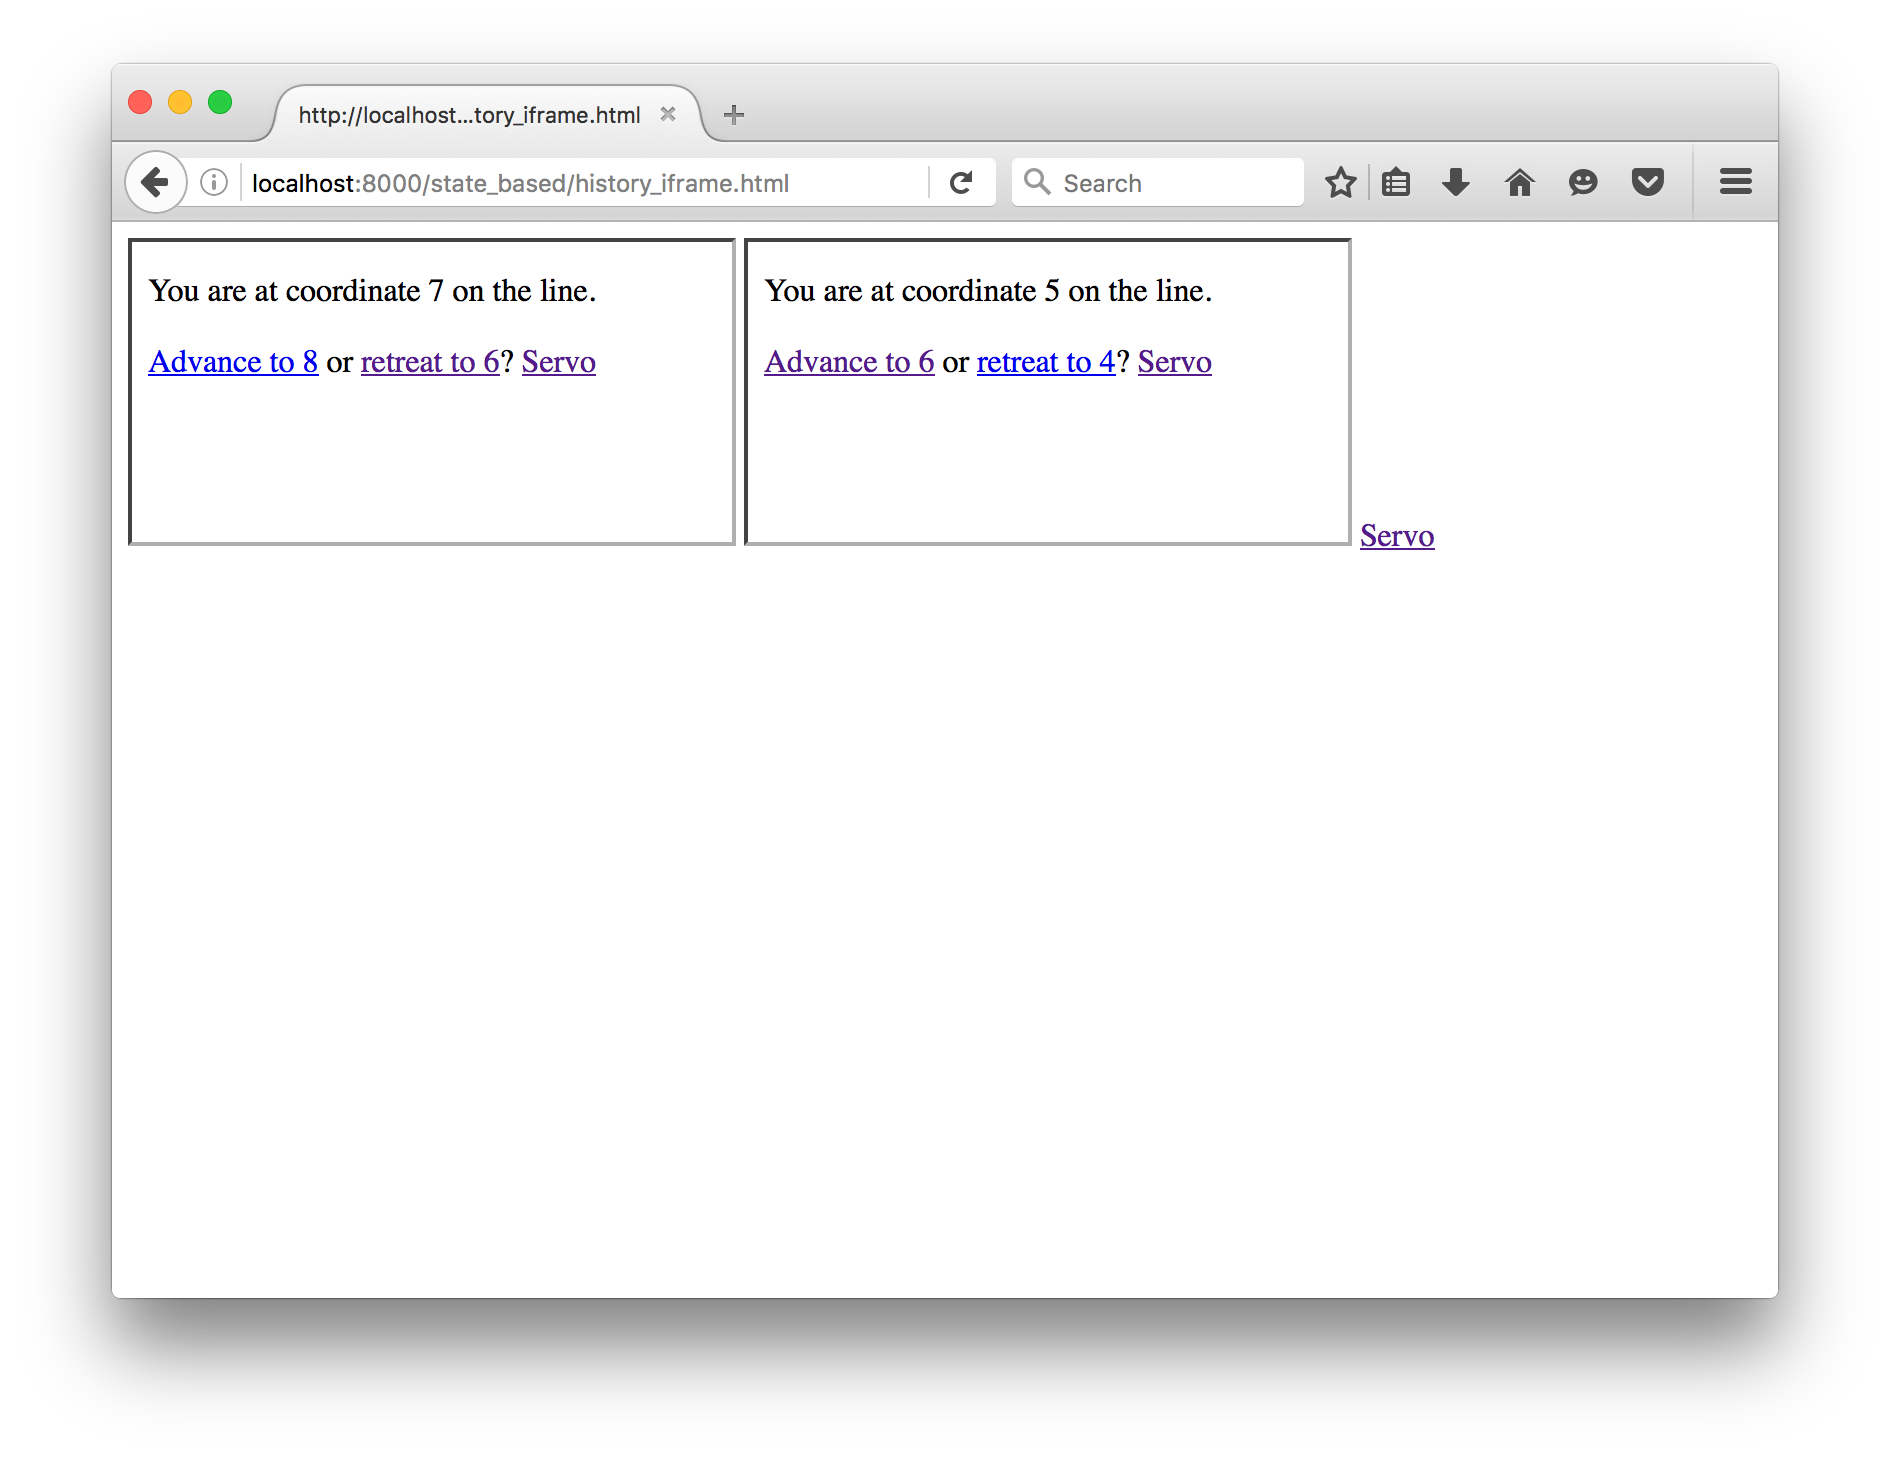
\includegraphics[width=.5\linewidth]{images/experiments/forwardback4state/firefox/7.png}%
    }~\raisebox{-.5\height}{
      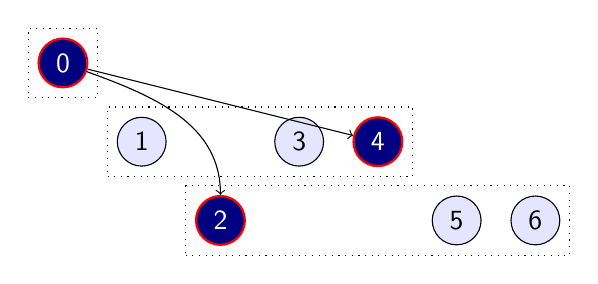
\begin{tikzpicture}
        \node[doc,active,fully](0) at (0,0){0};
        \node[doc](1) at (1,-1){1};
        \node[doc,active,fully](2) at (2,-2){2};
        \node[doc](3) at (3,-1){3};
        \node[doc,jshactive,fully](4) at (4,-1){4};
        \node[doc](5) at (5,-2){5};
        \node[doc](6) at (6,-2){6};
        \node[draw,dotted,fit=(0)]{};
        \node[draw,dotted,fit=(1)(4)]{};
        \node[draw,dotted,fit=(2)(6)]{};
        \draw[->](0)--(4);
        \draw[->](0)to[out=-20,in=90](2);
      \end{tikzpicture}
    }
    \caption{Traverse $\aNH$ by $4$}
  \end{figure}

  The last traversal does not satisfy Goal~\ref{goal:homomorphism}.

\end{experiment}

\section{Specification}

[Suggested edits to the spec:
  1. traverse to each document, not just the selected one,
  2. keep all documents in the seession history, not just the fully active ones,
  3. change the session history order.]

\section{Conclusion}

[We did stuff.]

\end{document}
